%%%%%%%%%%%%%%%%%%%%%%%%% DISCLAIMER %%%%%%%%%%%%%%%%%%%%%%%%%
% Die Kommentare sind tatsächlich nur für mich - sollen mich aber nicht davon abhalten, das Ding hier zu veröffentlichen, nur weil die Qaulität des Codes sowohl amateurhaft, als auch null für die Veröffentlichung aufbereitet ist und die Sprache der Kommentare nicht veröffentlichungstauglich ist.
%%%%%%%%%%%%%%%%%%%%%%%%%%%%%%%%%%%%%%%%%%%%%%%
\documentclass[a4paper, 
    12pt, 
    ngerman, 
    listof=totoc,
    titlepage]{scrartcl} % a4paper, damit nicht amerik. letterpaper; 12pt Schriftgröße; ngerman Umlaute äöü oder sowas; titlepage damit keine Seitenzahl bei Titelseite, \subject etc. dazugeknallt werden können, hübscher isses auch; scratrcl soll deutsch und hübsch sein, hat aber keine chapter nur section, aber chapter fangen auch neue Seiten an https://texwelt.de/fragen/15869/seitennummer-in-scrartcl-auf-titelseite-unterdrucken
% hatte bis 2025-05-14 a4paper in [] nach springer nature vorlage habe ich da mal pdflatex reingeschrieben, scheint nix kaputt zu machen. Ich glaube KOMA script mit scrartcl sollte sich schon um DIN A4 kümmern

\usepackage[utf8]{inputenc} % moderner Zeichencode, auch mit ä ö ü und so'n Kram
\usepackage[T1]{fontenc} % font encoding. T1 is best for west european e.g. due to hyphenation - Schriftarten gute diese glaube ich
\usepackage{lmodern} % latin modern Serif Font based on the older Computer Modern - hübsche Schrift? hab's vergessen

\usepackage[ngerman]{babel} % Sprache, ngerman Silbentrennung nach neuer Rechtschreibung und so
% \usepackage{verbatim} % das habe ich gefunden um ganze Blöcke inklusive Zeilenumbrüchen auszukommentieren -- Nachtrag lol, bullshit, verbatim direkt druckt code ohne auszuführen
% \usepackage[normalem]{ulem} % zum Durchstreichen https://texwelt.de/fragen/3223/wie-kann-ich-text-durchstreichen ulem besser wegen äöüß und neuer. soul besser als ulem für Zeilenumbrüche, Zeilenumbrüche bei Links waren nicht existent mit ulem https://tex.stackexchange.com/questions/74893/strikeout-when-which-package-ulem-vs-soul-vs#comment710882_74910 ich versuche also ulem mit normalem als Option https://golatex.de/viewtopic.php?t=3079 prima, scheint zu klappen

% \usepackage{acronym} % added 2024-06-05 https://www.heise.de/tipps-tricks/Abkuerzungsverzeichnis-in-LaTeX-erstellen-4982473.html oder https://de.wikibooks.org/wiki/LaTeX-W%C3%B6rterbuch:_Abk%C3%BCrzungsverzeichnis wiki empfiehlt womöglich package glossaries, hab da gerade kein Bock zu, acronym tut's bestimmt auch https://www.overleaf.com/learn/latex/Glossaries
% printonlyused could be put in []
% [v2 used because compile time in overleaf free]
% I try \usepackage{glossaries} 2025-06-03
\usepackage{amsmath}

\usepackage[onehalfspacing]{setspace} % Zeilenanbstand, Grüße ans Kompendium
\usepackage{geometry} % Seitenränder, ein wahrer Krampf
\geometry{
    left=30mm, 
    right=30mm, 
    top=25mm, 
    bottom=25mm
    } % mm besser als cm, bestimmt wegen , und . als Dezimaltrennzeichen, der Krampf hat sich entspannt, mm rulez
\usepackage[
    autostyle=true, 
    german
    ]{csquotes} % für Anführungszeichen in Zitaten in versch. Sprachen, Schachtelung und so: https://www.namsu.de/Extra/pakete/Csquotes.html

\usepackage[
    backend=biber, 
    style=authoryear-icomp, 
    bibstyle=authoryear, 
    dashed=false, 
    maxcitenames=2, 
    maxbibnames=99, 
    block=none
    ]{biblatex} % Zitationsstil, authoryear kommt Harvard nah -- date=year von Antwort aus https://texwelt.de/fragen/27027/zitationsstil-anpassen-biblatex-authoryear
% 2025-04-22 block=nbpar wäre erklärt bei Seite 51 von der Anleitung 3.1.2.1 https://mirrors.ibiblio.org/CTAN/info/translations/biblatex/de/biblatex-de-Benutzerhandbuch.pdf

\addbibresource{references.bib} % Bibliographie erstellen
% wenn unter Zitation -> Latex Assistant F7 ausgegraut, dann: Extras > Optionen > Zitation, da LaTeX anklicken
% im Moment (2022-09-06) ist TeXStudio angegeben und: quote; autocite; cite; parencite & quote; autocite; cite; parencite
% inspiriert von: https://help.citavi.com/topic/latex-assistent-kopieren
% stil authoryear-icomp s. Handbuch Seite 77 https://mirrors.ibiblio.org/CTAN/info/translations/biblatex/de/biblatex-de-Benutzerhandbuch.pdf
% 2025-04.02 maxbibnames=99 aus [] von biblatex genommen, da standard wohl =maxnames ist, Anleitung S. 49... Ok, doch nicht, gibt dann Fehler. vierlleicht lieber =99, weil ich die Schrägstriche definiert habe? Und sorting=nyt etnfernt, sollte Standard sein. Und dashed=false hinzugefügt Anleitung zu bibtex S. 81 bei Bibliographiestile
% hier steht auch maxbibnames=99 ist beste: https://tex.stackexchange.com/questions/12806/guidelines-for-customizing-biblatex-styles

% erst Nachname, dann Vorname https://www.mrunix.de/forums/showthread.php?75128-Biblatex-Nachname-Vorname klappt nur leider auch mit family-given nicht 2025-04-02 \DeclareNameAlias{default}{family-given}
% 2025-04-02 ohne ist nur beim ersten in der Bibliography der Nachname zu Beginn, danach ist es Vorname Nachname 

% https://texwelt.de/fragen/29060/biblatex-nachname-vorname default durch author (und editor und translator) ersetzt
\DeclareNameAlias{author}{family-given} % 2025-05-28 scheint nur author zu ändern, bei editor bleibts, daher: 
\DeclareNameAlias{editor}{family-given}
% \DeclareNameAlias{editor}{sortname}
% \DeclareNameAlias{translator}{sortname}

%%%%%%%%%%%%%%%% %%%%%%%%%%%%%%%% %%%%%%%%%%%%%%%% 
%%% von copilot für prompt: 
% wie verändere ich textcite in biblatex so, dass alle namen mit komma und und aufgezählt werden?
% \DeclareDelimFormat{andothersdelim}{\addcomma\space}
% \DeclareDelimFormat{finalnamedelim}{\space und\space}
% \DeclareDelimFormat{multinamedelim}{\addcomma\space}
%scheint aber nix zu ändern 2025-05-28

%%% von copilot für prompt: 
% das hat noch nicht geklappt. ich nuze folgenden stil: \usepackage[backend=biber, style=authoryear-icomp, bibstyle=authoryear, dashed=false, maxcitenames=2, maxbibnames=99]{biblatex}
% \DeclareDelimFormat{finalnamedelim}{\space und\space}
% \DeclareDelimFormat{multinamedelim}{\addcomma\space}
%scheint aber nix zu ändern 2025-05-28
%%%%%%%%%%%%%%%% %%%%%%%%%%%%%%%% %%%%%%%%%%%%%%%% 

\DefineBibliographyStrings{german}{
   andothers = {{et\,al\adddot}},
} % damit wird u.a. zu et al. siehe https://tex.stackexchange.com/questions/236854/changing-u-a-of-german-to-et-al

% no p. pp. and : instead of ,
% https://stackoverflow.com/questions/58448860/how-can-i-add-colons-and-remove-p-pp-from-in-text-citations-with-biblatex
\DefineBibliographyStrings{german}{
  page             = {},
  pages            = {},
}  % ich habe german anstatt english ergänzt % 2025-05-27 auf ngmerman geändert
% colon instead of comma bei in text cite
\renewcommand{\postnotedelim}{\addcolon \addspace} % \addspace kommt von mir
%%%%% 2025-06-30 I try german instead of ngerman -- doesnt solve warning, but works as well %%%%%%%%%%%%%%%

% no p.von anderer Quelle
% \DeclareFieldFormat{postnote}{#1}
% \DeclareFieldFormat{multipostnote}{#1}

\renewcommand*{\multinamedelim}{\addslash}
\renewcommand*{\finalnamedelim}{\multinamedelim}
% Schrägstriche zur Abtrennung https://golatex.de/viewtopic.php?t=18487 andere Quelle (hat nicht auf Anhieb funktioniert) https://groups.google.com/g/de.comp.text.tex/c/eSVMHAMphCA

%%%%%%% danke copilot
% Spezielle Anpassung für textcite
\DeclareDelimFormat[textcite]{finalnamedelim}{\space und\space}
\DeclareDelimFormat[textcite]{multinamedelim}{\addcomma\space}

% S. im Literaturverzeichnis wäre nett. da stehen hundert Zahlen hintereinander
%\renewbibmacro*{volume+number+eid}{%
%  \printfield{volume}%
%  \iffieldundef{volume}{}{~Aufl.}%
%  \setunit*{\addcomma\space}%
%  \printfield{number}%
%  \setunit*{\addcomma\space}%
%  \printfield{eid}}

%\renewbibmacro*{pages}{%
%  \iffieldundef{pages}{}{S.\space\printfield{pages}}}
%%%%%%%%%%%%%

% doppelte Nachnamen wegen shorthands (auto. durch citavi erstellt) in den refenerces.bib https://golatex.de/viewtopic.php?t=13563
% keine KURZBELEGE in CITAVI für Harvard Zit. verwenden!! https://www1.citavi.com/sub/manual6/de/index.html?cse_customizing_citation_keys.html

% \usepackage{minitoc} %h Mini Inhaltsverzeichnis https://cs.brown.edu/about/system/managed/latex/doc/minitoc.pdf
% \usepackage{pdfpages} % vielleicht mal pdfs direkt hier als anhang einbinden https://texwelt.de/fragen/19153/pdf-dateien-in-anhang-einbinden-aber-formatierung-des-vorhergehenden-dokuments-ubernehmen
% \usepackage{subfiles} % Best loaded last in the preamble https://de.overleaf.com/learn/latex/Multi-file_LaTeX_projects%23The_subfiles_package


%%%%%%%%%%%%%%%%%%%%%%%%%%%%%%%%%%%%%%%%%%%%%%%%%%%%%%%%%%
\newenvironment{myitemize} % https://tex.stackexchange.com/questions/10684/vertical-space-in-lists 2025-06-29
{ \begin{itemize}
    \setlength{\itemsep}{0pt}
    \setlength{\parskip}{0pt}
    \setlength{\parsep}{0pt}
    % \setlength{\baselineskip}{0pt}
    % \setlength{\topsep}{2pt}    % space before and after the list
    % \setlength{\partopsep}{0pt} % extra space added to \topsep when environment starts a new paragraph
 }
{ \end{itemize} } 

\newenvironment{myenumerate}
{ \begin{enumerate}
    \setlength{\itemsep}{0pt}
    \setlength{\parskip}{0pt}
    \setlength{\parsep}{0pt}
    % \setlength{\baselineskip}{0pt}
 }
{ \end{enumerate}                } 
%%%%%%%%%%%%%%%%%%%%%%%%%%%%%%%%%%%%%%%%%%%%%%%%%%%%%%%%%%%%%%

%%%%%%%%%%%%%%%%%%%%%%%%%%%%%%%%%%%%%%%%%%%%%%%%%%%%
\usepackage{graphicx}   % PDF Support % vorher war hier auch [pdftex] eingebunden. Nachdem ich hyperref in der Präambel nach unten geschoben habe, hat overleaf aber einen Fehler ausgespuckt
\usepackage{float} % addded 2025-06-10
% hier war mal \usepackage[hidelinks]{hyperref} % Hyperlinks % hidelinks keine bunten Kasten um klickbare Elemente: https://texwelt.de/fragen/1121/wie-entferne-ich-die-roten-rahmen-um-hyperlinks? 2025-05-14 ist jetzt nach unten gerutscht 2025-06-19
% \usepackage{times}              % Font fuer PDF besser % 2025-07-01 vielleicht doch lieber beim Standard bleiben: https://tex.stackexchange.com/questions/182906/ugly-usepackagetimes-examples % außerdem habe ich oben schon \usepackage{lmodern} eingebunden
\usepackage{thumbpdf}           % PDF Thumbnails erstellen
% https://www.linux-community.de/ausgaben/linuxuser/2005/04/mit-pdflatex-bessere-pdf-dateien-erzeugen/2/  
% 2025-05-14
%%%%%%%%%%%%%%%%%%%%%%%%%%%%%%%%%%%%%%%%%%%%%%%%%%%%

%%%%%%%%%% TABELLEN %%%%%%%%%%%%%%%%%%%%%%%%%
\usepackage{booktabs}
\usepackage{array}
% \usepackage{tabularx} % columns with X behave better
% \usepackage{longtable} % tables over several pages are possible
% \usepackage{ltablex} % should combine usepackage{tabularx} and \usepackage{longtable}
\usepackage{xcolor} % several colors available, needed for nice color options in \usepackage{tabularray} e.g.
\usepackage{tabularray} % this does everything tabularx and longtable can and even more, requires LaTeX3 (which is included in TeXLive e.g.)
%%%%%%%%%%%%%%%%%%%%%%%%%%%%%%%%%%%%%%%%%%%%%

%%%%%%%%%% LANDSCAPE %%%%%%% UND PDF EINBINDEN %%%%%%%
\usepackage{pdflscape} % I think I need this to have pdf pages in landscape orientation, to fit more pages on on a4paper
\usepackage[]{pdfpages} % very nice options to insert pdf once you understand them

\hyphenation{Durch-schnitts-ein-kommen}


\usepackage[
    xindy, 
    toc, 
    acronym,
    nomain, % ergänzt nach file main.glo which said main.gls is empty 
    nopostdot,
    nogroupskip
    ]{glossaries}
% xindy weil: https://tex.stackexchange.com/questions/199211/differences-between-xindy-and-makeindex/199841#199841
% https://en.wikibooks.org/wiki/LaTeX/Glossary#cite_note-2

    \newacronym{abb}{Abb.}{Abbildung}
    \newacronym{abs}{Abs.}{Abschnitt}
    \newacronym{ank}{ANK}{Arbeitnehmerkammer Bremen}
    \newacronym{arbschg}{ArbSchG}{Arbeitsschutzgesetz}
    \newacronym{bap}{bap}{Bundesausschuss Politische Bildung e.\,V.}
    \newacronym{bbk}{BBK}{Beutelsbacher Konsens}
    \newacronym{bgbl}{BGBl}{Bundesgesetzblatt}
    \newacronym{bmas}{BMAS}{Bundesministerium für Arbeit und Soziales}
    \newacronym{bpb}{bpb}{Bundeszentrale für politische Bildung}
    \newacronym{bspw}{bspw.}{beispielsweise}
    \newacronym{bzw}{bzw.}{beziehungsweise}
    \newacronym{c}{\copyright}{Copyright}
    \newacronym{diw}{DIW}{Deutsches Institut für Wirtschaftsforschung e.\,V.}
    \newacronym{doi}{DOI}{Digital Object Identifier}
    \newacronym{ebd}{ebd.}{ebenda}
    \newacronym{etc}{etc.}{et cetera}
    \newacronym{eu}{EU}{Europäische Union}
    \newacronym{gp}{GP oder GuP}{Gesellschaft und Politik}
    \newacronym{gpje}{GPJE}{Gesellschaft für Politikdidaktik und politische Jugend- und Erwachsenenbildung}
    \newacronym{idr}{i.\,d.\,R.}{in der Regel}
    \newacronym{ki}{KI}{Künstliche Intelligenz}
    \newacronym{kmk}{KMK}{Kultusministerkonferenz}
    \newacronym{lis}{LIS}{Landesinstitut für Schule}
    \newacronym{llm}{LLM}{Large Language Model}
    \newacronym{me}{m.\,E.}{meines Erachtens}
    \newacronym{nw}{NW}{Naturwissenschaften}
    \newacronym{ocr}{OCR}{Optical Character Recognition}
    \newacronym{oä}{o.\,Ä.}{oder Ähnliche(s)}
    \newacronym{s}{s.}{siehe}
    \newacronym{S}{S.}{Seite}
    \newacronym{sgb}{SGB}{Sozialgesetzbuch}
    \newacronym{sek}{Sek.}{Sekundarstufe}
    \newacronym{suub}{SuUB}{Staats- und Universitätsbibliothek Bremen}
    \newacronym{sus}{SuS}{Schülerinnen und Schüler}
    \newacronym{ua}{u.\,A.}{unter Anderem}
    \newacronym{url}{URL}{Universal Ressource Locator }% (einheitlicher Ressourcen Verorter, Webadressen)
    \newacronym{uu}{u.\,U.}{unter Umständen}
    \newacronym{vgl}{vgl.}{vergleiche}
    \newacronym{wuk}{WUK}{Welt-Umweltkunde}
    \newacronym{zap}{zap}{Zentrum für Arbeit und Politik}
    \newacronym{zb}{z.\,B.}{zum Beispiel}
    \newacronym{zit}{zit.}{zitiert}
    \newacronym{zt}{z.\,T.}{zum Teil}

\makeglossaries % das makeglossaries muss vor \begin{document} stehen, damit es funktioniert
% open Console in Visual Studio Code -- STRG+J click Console -- type: makeglossaries main (main being main.tex without extension) if no glossary with abbreviations appears

\usepackage[hidelinks=true,
            pdftitle=Chancen und Risiken von Fremdmaterial_Eine beispielhafte Analyse und Wertung von Unterrichtsmaterial der Arbeitnehmerkammer Bremen für den Politikunterricht an berufsbildenden Schulen in Bremen,
            pdfauthor=Paul Aljsocha Klein,
            pdfsubject=Masterarbeit Universität Bremen,
            pdfcreator=Paul Aljsocha Klein with LaTeX,
            pdfcreationdate=16.07.2025]{hyperref} % Hyperlinks % hidelinks keine bunten Kasten um klickbare Elemente. Das ist rausgenommen, weil keine Leerzeile unter Literatureinträgen: , backref=true, pagebackref=true
\begin{document}
\titlehead{
    
\includegraphics[width=0.5 \linewidth]{
    UniBremen_Logo_Rot-Schwarz_Web_NICHT_VERAENDERN.png
    }
}

\subject{
    Masterarbeit \\
    \normalsize
    zur Erlangung des akademischen Grades \\ 
    \emph{Master of Education} (M.Ed.) \\ 
    \bigskip 
    \url{github.com/gargardos/MA2025}
    }

\title{
    Chancen und Risiken von Fremdmaterial
    } 

\subtitle{
    Eine beispielhafte Analyse und Wertung von Unterrichtsmaterial der Arbeitnehmerkammer Bremen für den Politikunterricht an berufsbildenden Schulen in Bremen
    }

\author{
    Paul Aljoscha Klein\\ 
    \normalsize
    $\ast$ 20.07.1995\\ 
    \normalsize
    $\#$ 4134166
    }

\date{Abgabe: 16. Juli 2025}

\publishers{
    \vfill % doesn't seem to help
    \raggedright{
    Erstgutachter: Prof. Dr. Andreas Klee\\
    Zweitgutachterin: Dr. Eva Anslinger
    } 
    \hfill % bigger graphic-width inserts bigger vertical space between the two lines with the names. hfill doesn't really help % hfill seems unnecassary due to raggedleft, but without, the second name line gets pulled right
    \raggedleft{
    
\includegraphics[width=0.2 \linewidth]{
    zap_Logo_Website.001.png % Bildquelle: https://www.uni-bremen.de/fileadmin/user_upload/sites/soha/zap_Logo_Website.001.png 2025-06-19
    }
    } % raggedleft is needed in this setup
    }


% So sieht's gut aus mit titlepage bei Dokumentklasse scartcl, Danke Markus Kohm

%%%%%%%%%%%%% TitelBrainStorming %%%%%%%%%%%%%%%%%%%%%%%%%
% Nutzung von fremden Unterrichtsmaterialien. Eine exemplarische Analyse für den Politikunterricht an berufsbildenden Schulen in Bremen
% Nutzung von Unterrichtsmaterialien einer externen Institution. Eine exemplarische Analyse für den Politikunterricht an berufsbildenden Schulen in Bremen

% Entwürfe 2025-03-04 Di.
% Nutzung von fremden Unterrichtsmaterialien. Eine exemplarische Analyse für den Politikunterricht an berufsbildenden Schulen in Bremen

% Analyse und Wertung von großflächig angelegtem Unterrichtsmaterial Materialvorlagen: Exemplarisches Vorgehen mit Material der Arbeitnehmerkammer Bremen.

% Analyse und Wertung von Materialvorlagen für den Politikunterricht an berufsbildenden Schulen in Bremen: Eine beispielhafte Analyse mit Material der Arbeitnehmerkammer Bremen.

% Gekürzt:
% Analyse und Wertung von Materialvorlagen: Eine beispielhafte Analyse anhand von Unterrichtsmaterial für den Politikunterricht an berufsbildenden Schulen in Bremen der Arbeitnehmerkammer Bremen.

% Die Realität der Nutzung von institutionellem Unterrichtsmaterial entgegen selbsterstelltem Material: Eine beispielhafte Analyse anhand von Unterrichtsmaterial der Arbeitnehmerkammer Bremen für den Politikunterricht an berufsbildenden Schulen in Bremen.

% Nur selbsterstelltes Unterrichtsmaterial? Chancen und Risiken von Fremdmaterial: Eine beispielhafte Analyse und Wertung von Unterrichtsmaterial der Arbeitnehmerkammer Bremen für den Politikunterricht an berufsbildenden Schulen in Bremen.

% Unterricht von der Stange? Chancen und Risiken von Fremdmaterial: Eine beispielhafte Analyse und Wertung von Unterrichtsmaterial der Arbeitnehmerkammer Bremen für den Politikunterricht an berufsbildenden Schulen in Bremen

% Kriterien zur Bewertung von externen Unterrichtsmaterialien im Politikunterricht. Am Beispiel 
% Geschenke nimmt man gerne an
% Unterricht von der Stange
% Erleichterung durch fertiges Unterrichtsmaterial
%%%%%%%%%%%%%%%%%%%%%%%%%%%%%%%%%%%%%%%%%%%%%%%%%%%%%%%%%%%%%%%%%
\maketitle
\clearpage

\pagenumbering{roman}
\addsec{Abstract}
blub
Bre steht das hier auch in vsc?

\clearpage
\newpage

\tableofcontents % war früher mal vor pagenumbering. Macht das einen Unterschied? Keine AHnung 2024-06-05 ah ja, will ja nicht das Inhaltsverzeichnis Seitenummeriert haben 2024-06-06

% \clearpage
% \newpage

\listoffigures % Abbildungsverzeichnis
\listoftables % Tabellenverzeichnis

\printacronyms[type=\acronymtype, 
    nonumberlist, 
    title=Abkürzungsverzeichnis, 
    toctitle=Abkürzungsverzeichnis]{} % Acronymtype ist von glossaries, title und toctitle sind Titel im Inhaltsverzeichnis
% listof=totoc in \documentclass[] replaces %% , title={Abkürzungsverzeichnis}, toctitle={Abkürzungsverzeichnis} %% here
% \vspace{24pt} % vertical space

\clearpage
\newpage

\setcounter{page}{1}
\pagenumbering{arabic}
\section{Einleitung \& Theoretischer Hintergrund}
% Unterrichtsmaterial kommt nicht nur aus Schulbüchern oder wird von den Lehrkräften selbst erstellt

\subsection{Von der Theorie in die Praxis \label{theorie in praxis}}
Es gibt extensive Forschung in den Erziehungswissenschaften und der Fachdidaktik. Insbesondere der Bereich der politischen Bildung ist darüber hinaus mit zahlreichen interdisziplinären Brücken in die Sozialwissenschaften und über einen schulischen Bildungsbegriff hinaus ein Forschungsfeld, welches in seiner Gänze nicht einmal von Menschen zu überblicken ist, die ihr ganzes (Arbeits-)Leben der politischen Bildung gewidmet haben. 

Gleichzeitig sind sowohl die Möglichkeiten zur weiteren Erforschung als auch der konkrete Forschungsbedarf im Detail von nicht zu überblickender Größe. 
% explizit einschließt, dass mindestens genauso viel unerforscht ist und vieles sicherlich sinnvoll wäre zu erforschen. 

In unserer hochkomplexen Welt gilt dies sicherlich für das Gros an Forschungsbereichen. Die Eingrenzung und damit Abgrenzung von Forschungsgegenständen ist daher stets zwangsläufiger Bestandteil des Forschens. In der Praxis bedeutet das, immer wieder aushandeln zu müssen, inwieweit Querverbindungen zu anderen Bereichen notwendig sind und an welcher Stelle der Fokus wieder auf das Wesentliche zu legen ist.
Diese Entscheidungen sind optimalerweise nachvollziehbar zu begründen. Getroffen werden müssen sie dennoch. Das ist sicherlich mit Arbeit verbunden. 

Analog zu den Entscheidungen, die Forschende treffen müssen, um handlungsfähig zu sein, das heißt fokussiert ihre Forschung vorantreiben zu können, ist die begründete Eingrenzung eines Lerngegenstandes ebenfalls mit Entscheidungen verbunden. 
Lehrende befinden sich diesbezüglich also in einer ähnlichen Situation wie Forschende. 

Es ließe sich allerdings argumentieren, dass die Notwendigkeit im Unterrichten von Weltwissen Entscheidungen zu treffen -- wie es im Schulkontext stattfindet -- auf einer vageren Datengrundlage stattfindet. In der Forschung wird sich wegen der zuvor beschriebenen Notwendigkeit der Eingrenzung zunehmend spezialisiert. Im schulischen Weltverstehen-Lernen hingegen ist in weiten Teilen (noch) kein hochspezialisiertes Verständnis gefordert. Stattdessen steht ein allgemeines Zusammenhänge-verstehen-Lernen im Vordergrund. Das setzt Lernen an exemplarischen Lerngegenständen voraus. 
Dies gilt insbesondere für die politische Bildung -- nicht nur in allgemeinbildenden Schulen, sondern auch für Politikunterricht in der dualen Berufsbildung \autocite[vgl. \gls{abs} \ref{bplan}: \gls{S} \pageref{bplan} \&][4; 9-13]{bplan}.
In der Ausbildung zum Lehramt wird Wert darauf gelegt, solche Entscheidungen, welche Lerngegenstände ausgewählt werden, umfassend begründen zu können. 
In der Praxis des Lehrens wird Wert darauf gelegt, tatsächlich zu unterrichten.
In der wissenschaftlichen Literatur wurde dieses ständige im Widerspruch stehen, dem Lehrkräfte an verschiedenen Stellen ausgesetzt sind, längst erkannt und als Antinomie bezeichnet \autocite[\gls{vgl} \gls{zb}][]{Helsper.2001}.

Den kompletten Wissensstand der unterrichteten Domäne von einzelnen Lehrkräften fachwissenschaftlich oder didaktisch im kompletten Überblick zu behalten, ohne dass Teile des Alltagsgeschäfts hintenüber fallen, erschiene daher als eine utopische Forderung. Daher erscheint die Benutzung von vorgefertigtem Unterrichtsmaterial eine praktikable Erleichterung. 

% HIER NOCH MEHR BRÜCKE ZU ARBEITSERLEICHTERUNG SCHLAGEN. MATERIALERSTELLUNG UNGLEICH UNTERRICHTEN

Entsprechend ist es eine willkommene Abwechslung, in dieser Arbeit zwar nicht zur Erleichterung des Handwerks des Unterrichtens beizutragen, wohl aber eine Initiative zum Untersuchungsgegenstand zu haben, der genau diese Intention unterstellt werden kann. 

\subsection{Lerngegenstände}
Die \gls{kmk} definiert \emph{Lehr}mittel als Materialen der Schule und \emph{Lern}mittel als Materialien der Schüler*innen \autocite{KMKMittel}. Gerade im Hinblick auf Verbrauchsmaterial und dessen Finanzierung ist das bestimmt eine sinnvolle Unterscheidungsdimension. Papier und Stifte stammen in der Regel von Schüler*innen, die abbrechende Bohrerspitze im Werkunterricht und % die Objektträger zur Mikroskopie 
das Gas zur Erhitzung der Chemikalie im Naturwissenschaftsunterricht, sind häufig aus der Schule oder werden auch mal aus den privaten Ressourcen der Lehrkräfte finanziert. Herausgestellt werden soll, dass Lernen in weiten Teilen in Verbindung mit der dinglichen Welt stattfindet.

Unterrichten an Bildungsinstitutionen passiert hauptsächlich unter Zuhilfenahme von Medien im engeren Sinne. Die Planung ist im besten Fall verschriftlicht oder anderweitig aufgezeichnet, \gls{zb} durch Grafiken. Die Planung des Unterrichts und die Auswahl oder Erstellung der zum Unterrichten verwendeten Materialien nehmen dabei einen erheblichen Zeitaufwand seitens der Lehrkräfte ein.

Das Zurückgreifen auf bestehende Medien ist dabei natürlicher Bestandteil des Lernens. So ist die (Primär-)Quellenanalyse im Geschichtsunterricht, das Lesen eines Haikus in Deutsch, die Analyse einer Inszenierung, das Basteln an einem Motor oder das Erhitzen von Chemikalien die natürliche Benutzung von Unterrichtsmaterial. 


Um diversen Gegebenheiten gerecht zu werden, ist das Material jedoch häufig abstrahiert. Eine Dampfmaschine steht womöglich nicht zur Verfügung. In so einem Fall kann \gls{zb} auf eine Explosionszeichnung, einen Film, ein Modell oder eine Beschreibung zurückgegriffen werden. Eine Beschreibung in Worten erfordert dabei eine höhere Abstraktionsebene als ein Modell und birgt die Gefahr, schlechtere Lernergebnisse zu erzielen; was dann durch entsprechende Einbettung oder die Ergänzung weiterer Materialien, wie einem Schema oder einem Film, versucht werden sollte zu kompensieren. Wie anhand dieses Beispiels bereits deutlich wird, erfordert bereits die Auswahl der Lehrmaterialien Arbeit, bevor überhaupt mit den Lernenden in Interaktion getreten wird. 
Wenn nun in der politischen Bildung eine Rede analysiert wird, sind die naheliegenden Möglichkeiten überschaubar. Eine Verschriftlichung und eine Videoaufnahme bieten sich an. 

Gerade in der politischen Bildung liegt der Lerngegenstand jedoch häufig auf noch ferner liegenden Abstraktionsebenen. Es geht um hochkomplexe Konzepte (wie \gls{zb} \emph{Demokratie}), die in der physischen Welt schwer greifbar sind. Entsprechend viele nah- und fernliegende Möglichkeiten bestehen bei der Auswahl an Unterrichtsmaterial\footnote{Das soll nicht bedeuten, dass die Vorbereitungen im Mathematikunterricht zum ergänzenden Material einer eindeutigen Rechenaufgabe, \gls{zb} durch kleinschrittiges Vorgehen, grafische Darstellung oder Darstellungen in der physischen Welt, nicht ebenfalls hochkomplex sind und zahlreiche Entscheidungen erfordern. Aber viele Lerngegenstände der politischen Bildung sind an sich schon derart abstrahiert, dass dort die Beschäftigung mit der Darstellung unvermeidlich ist.}.

Unterrichtsmaterial, für welches bereits Entscheidungen bezüglich des exemplarischen Lerngegenstandes und der didaktischen Reduktion getroffen wurden, hat also gewaltiges Potential, eine Arbeitserleichterung darzustellen.
Beispielsweise indem es für die Zielgruppe und die Zielvorgaben aus einem Lernplan bereits vorausgewählt und für eine ansprechende Darstellung aufbereitet wurde.
Arbeit zieht jedoch auch vorgefertigtes Material nach sich, da die Beurteilung der Qualität und die Eignung sowie die Anpassung für die Lerngruppe keine Selbstverständlichkeit sind.

\paragraph{Herkunft der Lerngegenstände}
Die Notwendigkeit des Lernens, eben auch Lerngegenstände zu haben, hat entsprechend auch verschiedene Akteure mit unterschiedlichen Intentionen auf den Plan gerufen, welche Unterrichtsmaterial anbieten.
Einsteigend hervorzuheben sind dabei die privatwirtschaftlichen Schulbuchverlage, welche dem klassischen Bild von Unterrichtsmaterial entsprechen. Jedoch haben auch andere Institutionen das Potenzial einer Einflussnahme auf Lernende durch 
% geschickt gestaltetes 
Material entdeckt. Wirtschaftsverbänden oder großen Unternehmen kann dabei bisweilen eine andere Intention als eine altruistische unterstellt werden, die durch auf den ersten Blick kostenfreies Material verfolgt wird. So braucht man in der Forschung von Reinhold Hedtke bisweilen nicht weiter als bis zu den römischen Seitenzahlen zu lesen, um darauf zu stoßen, dass Schulen \enquote{sich zunehmend gegen weltanschauliches, wissenschaftliches, wirtschaftliches und politisches Lobbying aus Unternehmen und ihrem Umfeld wehren} müssen \autocite[i]{Hedtke2016}. 


Auch die \gls{ank} entwickelt in Kooperation mit dem \gls{zap} an der Universität Bremen Unterrichtsmaterial für den Politikunterricht.


In dieser Arbeit soll ein Versuch unternommen werden, dieses Unterrichtsmaterial zu analysieren und zu bewerten. % welches den Lehrkräften von dem quasi staatlichen Akteur der Arbeitnehmerkammer Bremen zur Verfügung gestellt wird. 

\subsection{Unterrichtsmaterial}
Der Begriff Unterrichtsmaterial soll in etwa synonym zur Definition auf der Website der \textcite{KMKMittel} für Lehr- und Lernmittel verwendet werden: 
Es gibt eine Lernmittelfreiheit \autocite[]{KMKMittel}.
Welches Unterrichtsmaterial am Ende auch in Kontakt mit den Schüler*innen kommt, liegt hauptsächlich in den Händen der Lehrer*innen.
Die Lehrkräfte selbst sind bei der Auswahl des Materials jedoch zahlreichen Zwängen ausgesetzt:
\begin{itemize}
    \item Zeitliche Zwänge: Der Tag hat nur 24 Stunden und Menschen sind Tiere mit zahlreichen biologischen und sozialen Bedürfnissen. Diese zu erfüllen ist Voraussetzung für eine gute Arbeitsleistung, nimmt jedoch, genau wie Arbeit selbst, Zeit in Anspruch. 
    \item Finanzielle Zwänge: Schulen stehen begrenzte Budgets zur Verfügung, z.B. sind Schulbücher häufig nicht die \enquote{besten} und aktuellsten am Markt und Exkursionen müssen für alle bezahlbar sein. 
    \item Bereits am Markt existierendes Material ist entweder kostspielig und/oder unterliegt nur unzureichenden Qualitätskontrollen. Die Prüfung und Umgestaltung, um im Unterricht eingesetzt werden zu können, nimmt wiederum viel Zeit in Anspruch. 
\end{itemize}

Unterrichtsmaterial wird häufig aus dem Internet bezogen \autocite[82]{Neumann2015}. % zitiert nach \autocite[66]{Hedtke2016}


\section{Theoretischer Hintergrund / Begriffsklärungen}
Um das Material zu analysieren, hilft es zunächst, mehrere Begriffe zu klären. Zum ersten eine Definition, was unter Unterrichtsmaterial verstanden werden soll und.... % Zum zweiten ein Überblick, wie politische Bildung an Berufsschulen in Bremen stattfindet. 
Dann sollen der Bildungsplan in Politik vorgestellt werden, sowie der \gls{bbk}, auf den jener Bezug nimmt. Um im späteren Verlauf die verschiedenen Lebensweltbezüge aufzeigen zu können, soll daraufhin noch die Zielgruppe der Lernenden umrissen werden. 
Blub blub, nur ausführen was die Überschriften weshalb sagen........
JA, DER BUMS IST UNABGESCHLOSSEN



% fick dich, ich bin Krebs 

\subsection{Politische Bildung an berufsbildenden Schulen in Bremen}
JA HIER FEHLT WAS, VIELLEICHT NEHME ICH DAS RAUS

\subsection{Beutelsbacher Konsens \label{bbk}}% Beeinflussung durch Material.
Da insbesondere durch die Schulpflicht \autocite{BremSchulG} die schulische (politische) Bildung mit Zwang verbunden ist, liegt es nahe, dass versucht wird, diese durch Regeln, trotz des Zwanges, mit freiheitlichen, demokratischen Grundwerten zu vereinbaren. Auch an Berufsschulen, für die das hier untersuchte Material primär entworfen ist, besteht noch ein starkes, strukturvorgegebenes Machtgefälle, welches derartige Überlgungen stets aktuell sein lässt. 

Ein wichtiges historisches Dokument im Rahmen derartiger Fragestellungen ist der \Acrlong{bbk} \autocites[29]{Gesner2016}{Wehling1977} -- so wichtig, dass auch über den deutschen Raum hinaus auf den \gls{bbk} Bezug genommen wird. So wurde im Rahmen der \emph{Aktionstage Politische Bildung} vom 23. April bis 9. Mai 2024 in Österreich formuliert, dass der \gls{bbk} \enquote{[v]on internationaler Bedeutung [...] ist [...]. \autocite{bbkÖsterreich2023}}. Entsprechend leitet auch der Bremer Bildungsplan zentrale Kompetenzen aus dem \gls{bbk} ab und gibt die wichtigste Stelle \enquote{im Wortlaut} wieder \autocite[11-12]{bplan}: 
\begin{quote}
    \textbf{1. Überwältigungsverbot.}

    Es ist nicht erlaubt, den Schüler - mit welchen Mitteln auch immer - im Sinne erwünschter Meinungen zu überrumpeln und damit an der \enquote{Gewinnung eines selbständigen Urteils} zu hindern. Hier genau verläuft nämlich die Grenze zwischen Politischer Bildung und Indoktrination. Indoktrination aber ist unvereinbar mit der Rolle des Lehrers in einer demokratischen Gesellschaft und der - rundum akzeptierten - Zielvorstellung von der Mündigkeit des Schülers. 

    \textbf{2. Was in Wissenschaft und Politik kontrovers ist, muss auch im Unterricht kontrovers erscheinen.}

    Diese Forderung ist mit der vorgenannten aufs engste verknüpft, denn wenn unterschiedliche Standpunkte unter den Tisch fallen, Optionen unterschlagen werden, Alternativen unerörtert bleiben, ist der Weg zur Indoktrination beschritten. Zu fragen ist, ob der Lehrer nicht sogar eine Korrekturfunktion haben sollte, d.h. ob er nicht solche Standpunkte und Alternativen besonders herausarbeiten muss, die den Schülern (und anderen Teilnehmern politischer Bildungsveranstaltungen) von ihrer jeweiligen politischen und sozialen Herkunft her fremd sind. Bei der Konstatierung dieses zweiten Grundprinzips wird deutlich, warum der persönliche Standpunkt des Lehrers, seine wissenschaftstheoretische Herkunft und seine politische Meinung verhältnismäßig uninteressant werden. Um ein bereits genanntes Beispiel erneut aufzugreifen: Sein Demokratieverständnis stellt kein Problem dar, denn auch dem entgegenstehende andere Ansichten kommen ja zum Zuge. 
    
    \textbf{3. Der Schüler muss in die Lage versetzt werden, eine politische Situation und seine eigene Interessenlage zu analysieren,} 

    sowie nach Mitteln und Wegen zu suchen, die vorgefundene politische Lage im Sinne seiner Interessen zu beeinflussen. Eine solche Zielsetzung schließt in sehr starkem Maße die Betonung operationaler Fähigkeiten ein, was eine logische Konsequenz aus den beiden vorgenannten Prinzipien ist. Der in diesem Zusammenhang gelegentlich - etwa gegen Herman Giesecke und Rolf Schmiederer - erhobene Vorwurf einer \enquote{Rückkehr zur Formalität}, um die eigenen Inhalte nicht korrigieren zu müssen, trifft insofern nicht, als es hier nicht um die Suche nach einem Maximal-, sondern nach einem Minimalkonsens geht. 
    
    \autocite[Im Original mit anderen Hervorhebungen:][179-180]{Wehling1977}
\end{quote}



\subsection{Bremer Bildungsplan \label{bplan}} % \& Kompetenzen in der politischen Bildung
Der aktuelle Bremer Bildungsplan für politische Bildung\footnote{Als Fach vom \gls{lis} nur als Politik bezeichnet} für berufsbildende Schulen ist mit der Erscheinung \citeyear{bplan} (\citeauthor{bplan}) vergleichsweise aktuell. Die Bremer Bildungspläne für politische Bildung an der \gls{sek} I und II der allgemeinbildenden Schulen sind alle etwa im vorletzten Jahrzehnt, zwischen \citeyear{vogel2006gy} \autocites{vogel2006gs, vogel2006gy, lower2008} und \citeyear{vogel2010gp} \autocite{vogel2010gp}, erschienen. Die Fächerbezeichnungen sind innerhalb der Bremer Bildungspläne nicht kongruent. Die unstete Bezeichnung der Fächer -- welche politische Bildung, häufig neben anderen Bereichen, mit abdecken -- wird in \gls{abs} \ref{polBildung}: (\gls{S} \pageref{polBildung}) weiter diskutiert.

Politik ist neben Deutsch im Jahr 2024/2025 aktuell das einzige andere Fach im Land Bremen, welches für den berufsbildenden Bereich fächerübergreifend für alle Schülerinnen und Schüler unterrichtet wird (vgl. Website des \gls{lis} \citeyear{LisBildungspläne}). Direkt im Bildungsplan \autocite[][4]{bplan} wird darauf eingegangen, dass zwar an \enquote{heterogene[...] Voraussetzungen der Schüler:innen} angeknüpft wird, was auch \enquote{die Unterschiedlichkeit der jeweiligen Bildungsgänge} berücksichtigen soll, aber als Teil der \enquote{allgemeinbildenden Fächer} sollen die \enquote{Zielsetzungen politische Urteilsfähigkeit, politische Handlungsfähigkeit und methodische Fähigkeiten} immer die Grundlage bilden. 


Allgemeine politische Kompetenzen sind die hauptsächlichen Ziele \autocite[9-13]{bplan}.

Für die \enquote{Kompetenzdimensionen in der politischen Bildung} orientiert sich der Bildungsplan stark an den Ausarbeitungen der \gls{gpje}.
Da in dieser Arbeit (\gls{s} \gls{abs} \ref{öffi}: \gls{S} \pageref{öffi}) auch auf die Verfügbarkeit und Nutzfreundlichkeit von Unterrichtsmaterial eingegangen wird, bietet es sich an, an dieser Stelle ein strukturelles Einzelfallbeispiel aufzuzeigen:

\subsubsection{Exkurs: Schlechte Quellenangaben und unzureichende Vorbildfunktion. Beginnt Medienkompetenz im Bildungsplan? \label{gpje}}
Der Bildungsplan selbstwird von fiskalisch finanzierten Stellen erarbeitet und für einen Bildungsbereich veröffentlicht, welcher sich auch als öffentlich versteht -- sowohl in Form von öffentlichen Geldern finanziert als auch in Form von öffentlich zugänglich -- da es sich um einen verbreiteten, staatlich vorgezeichneten \mbox{(Weiter-)Bildungsweg} % \mbox trennt Begriff nicht 
handelt. Der Bildungsplan ist auf der Website des \gls{lis} (\citeyear[]{LisBildungspläne}) auch öffentlich zugänglich im etablierten .pdf-Format vorzufinden und bietet allen Menschen die Möglichkeit, mit diesem öffentlich erarbeiteten Wissen zu arbeiten.
Soweit erscheint das Vorgehen kohärent und sinnvoll.

Der Bildungsplan orientiert sich \gls{ua} an den Bildungsstandards der \gls{gpje}. Konkret wird das \gls{ua} an Fußnote 13 im Bildungsplan \autocite[][9]{bplan} deutlich, vergleichbar zu folgender Fußnote\footnote{\url{http://gpje.de/wp-content/uploads/2017/01/Bildungsstandards-1.pdf}}. Da ein Zitierstil nicht nur kontextabhängig, traditionsabhängig und subjektiv ist, soll dahingehend selbstverständlicherweise keine Wertung stattfinden. Allerdings sind in diesem Fall bereits mehrere zitierstilübergreifende Grundsätze missachtet worden. Sich dafür zu entscheiden, einen Fußnotenzitierstil zu nutzen und an späterer Stelle ein komplettes Quellenverzeichnis, wäre eine solide Wahl. Auch wenn als dabei übliche Kurzform in der Fußnote ausschließlich einen kompletten Weblink anzugeben schon wild ist. Nur dass es schlicht kein komplettes Quellenverzeichnis gibt!  
Es gilt, ausreichend Informationen (lieber eine zu viel als eine zu wenig) zum Auffinden anzugeben, insbesondere und mindestens Äquivalente zu Autor*innen oder Herausgeber*innen, sowie Erscheinungsjahr und Titel und das Zugriffsdatum, falls Weblinks angegeben sind. 
Als findige*r Konsument*in von Text lassen sich nun Teile von Titel und Namen sowie das Akronym der Herausgebenden im Link herauslesen. Allerdings führt der Link im Mai 2025 auf eine weiße Seite und ist damit ein Paradebeispiel, weshalb \gls{ua} wenigstens ein Zugriffsdatum zur eigenen Absicherung angegeben sein sollte.

Als bemühter Autor einer universitären Abschlussarbeit findet man jedoch unter diesem Link\footnote{\url{https://gpje.de/publikationen/} (06.05.2025)} einen Download mit diesem Link\footnote{\url{https://gpje.de/wp-content/uploads/2024/07/Bildungsstandards-1.pdf} (05.05.2025)}, dessen \gls{url} entsprechend der Zahlen, die ein Datum darstellen könnten, womöglich eine aktuellere Version zu der im Bildungsplan \autocite[][9]{bplan} referierten verspricht. Laut Website und Untertitel soll es sich zwar lediglich um einen Entwurf handeln. Wobei \enquote{Entwurf} sich an dieser Stelle wohl eher als Synonym für \emph{Vorschlag} lesen lässt.  Das Dokument kann jedoch nach wie vor in seiner Veröffentlichungsform strukturell kritisiert werden:
\begin{itemize}
    \item Das in der \gls{url} suggerierte Datum impliziert nun eine Veröffentlichung oder Version vom Juli 2024, im Dokument selbst ist ein \gls{c} vom Wochenschau Verlag von 2004 angegeben. Es handelt sich höchstwahrscheinlich um eine Version der viel zitierten 2. Auflage von \citeyear[]{gpje2004}. Nur dass im Bildungsplan nicht ersichtlich ist, ob er sich tatsächlich auf diese Version bezieht. Höchstwahrscheinlich bezog sich die alte \gls{url}, in der \enquote{2017} zu lesen ist, auf dieselbe Version, wie die, welche hier mit \enquote{2024} in der \gls{url} aufgefunden wurde. 
    
    
    \item Es gibt keinen Versionsverlauf, auf der eigenen Website der \gls{gpje} ließ sich eine Version von 2017, wie die \gls{url} im Bildungsplan \autocite[][9]{bplan} suggeriert, nicht finden. Die Zahlen 2017 und 2024 scheinen in diesem Fall schlicht keine andere Version zu kennzeichnen. Denkbar ist, dass es nur intern erneut hochgeladen wurde.

    \item Wenn die \gls{url} nicht gerade eine \gls{doi} \gls{oä} ist, ist diese Fußnote als einzige Quellenangabe daher ein Paradebeispiel, weshalb meist schon zu Beginn einer universitären Ausbildung darauf hingewiesen wird, dass man sich nicht ausschließlich auf eine \gls{url} verlassen sollte. 
    
    \item Es gibt auch keine vernünftige Suchfunktion auf der Website. Eine miese Suchfunktion und intransparente, nicht anpassbare Sortierungen scheinen allerdings gerade bei Websites mit in Teilen fiskalischer Finanzierung Best Practice zu sein.
    
    Zur Verteidigung sei angemerkt, dass es sich in diesem Fall um eine gemeinnützige Organisation handelt. Dass bei solchen bisweilen die Ressourcen knapp sind, ist keine Seltenheit.  
    
    \item Das Dokument über die Bildungsstandards der \gls{gpje} ist soweit schreibgeschützt, dass sich Text nicht kopieren lässt. Besonders hinsichtlich der zahlreichen Möglichkeiten, den Kopierschutz auf verschiedenen Websites entfernen zu lassen -- um im Jahre 2025 nicht die Verlegenheit kommen zu müssen abzuschreiben -- erscheint das erstens unnötig und zweitens kontraproduktiv. Es kann dazu verleiten, das Dokument auf ohne große Prüfung hastig herausgesuchte Websites hochzuladen. Das wäre wahrscheinlich nicht die Intention, die mit dem Hinzufügen eines Kopierschutzes verfolgt wurde.
    
    \item In der Satzung der \gls{gpje} (\citeyear[]{gpje.satzung}) ist unter \enquote{\S 1 Zweck der Gesellschaft} zu lesen, dass es sich bei der Organisation um eine \enquote{wissenschaftliche Fachgesellschaft, die der Förderung der wissenschaftlichen Auseinandersetzung mit Fragen der schulischen und außerschulischen politisch-gesellschaftlichen Bildung in Forschung und Lehre dient} handelt.
    Ferner verfolgt die \gls{gpje} laut ihrer Satzung \blockquote{ausschließlich und unmittelbar gemeinnützige Zwecke [...] Sie leistet dies insbesondere durch:
    
    a. Förderung des wissenschaftlichen Diskurses, der Forschung und der wissenschaftlichen Kooperation,
    
    b.Veranstaltung von Fachtagungen und Kongressen,
    
    c. wissenschaftliche Publizistik,
    
    d. Intensivierung der europäischen und der internationalen wissenschaftlichen Zusammenarbeit,
    
    e. Förderung der Lehre an Hochschulen und die Förderung des wissenschaftlichen Nachwuchses,
    
    f. das wissenschaftlich-politische Engagement für den Ausbau der Disziplin an den Hochschulen.}

    Hinsichtlich der in der Satzung formulierten Ziele, weiß der Widerspruch zwischen Form und Inhalt humoristisch zu begeistern. Bildungsstandards einer wissenschaftlichen Gesellschaft, welche mit der Intention, von verschiedenen -- auch und insbesondere öffentlichen -- Bildungsinstitutionen genutzt zu werden, sind auf der eigenen Website schwer zugänglich (Kopierschutz), es gibt keine Suchfunktion und keinen stabilen Link (oder Versionsverlauf, wenn es sich um verschiedene Versionen handeln würde). Das erschwert wissenschaftlich korrektes Zitieren unnötig -- was sich tatsächlich auch in einem offiziellen Bildungsplan \autocite[][9]{bplan} niederschlägt, der diese Situation allerdings erst durch die unsaubere Arbeit derart verschärft hat. 
    
    \item Man stelle sich vor, man ist etwa Schüler*in, Lehrkraft, Elternteil oder Student*in und wirklich daran interessiert, in die Tiefe der Bildungsstandards einzusteigen, und ist soweit wie oben beschrieben gekommen -- dann kommt man möglicherweise auf die Idee sich sicherheitshalber die wissenschaftliche Publizistik der \gls{gpje} anzuschauen, um nachzuprüfen, ob es doch verschiedene und womöglich aktuellere Versionen gibt. Die Publizistik wird im Wochenschau Verlag vertrieben und ist nicht frei zugänglich. 
    
    Man könnte auf die Idee kommen, in einer Veröffentlichung von \citeyear{Gortler.2017} \gls{zb} (\citeauthor{Gortler.2017}) könnte ja eine passende Version von 2017 zu finden sein. Das auf Vertriebswebsites frei einsehbare Inhaltsverzeichnis reicht, um das zu verneinen. Was hilfreich ist. Denn auch wenn dem Band eine Tagung an der Universität Bremen von 2016 zur Grundlage liegt, ließen sich digitale (und physische) Versionen -- auch im Universitäts-Netzwerk der \gls{suub} eingeloggt sitzend -- nur gegen Geld erwerben. Die \gls{suub} besagter Bremer Uni führt immerhin ein physisches Exemplar auf Ebene 3 (Stand 06.05.2025). 

    \item An dieser Stelle ist dann womöglich ausreichend Sicherheit darin gefunden, dass die Version von \citeyear{gpje2004}, die aktuelle ist, auf die sich bezogen wird.

    \item Immerhin gibt es überhaupt eine kostenlose online Version und es müssen nicht tausende Menschen, die was mit dem Bildungssystem in Bremen am Hut haben, auf irgendein physisches Exemplar in einer Bibliothek verwiesen werden. % in der \gls{suub} verwiesen werden (Stand 30.05.2025).    
\end{itemize}
Einem Bildungssystem, dessen Regelungen und Grundlagen nicht hürdenarm, frei und öffentlich zugänglich sind, lassen sich nämlich strukturelle Unzulänglichkeiten im Rahmen einer freiheitlichen Demokratie unterstellen. 
% Es erschiene fast die Arbeitsbschaffungsmaßnahme des Müllsammelns sinnvoller, als sich durch einen derartigen Dschungel an Recherchearbeit schlagen zu müssen. Wenn es nur auch im Müllsammel-Beispiel nicht sinvoller wäre, die Umgebung so zu gestalten, dass Müll korrekt zu entsorgen niederschwelliger ist und damit eine höhere Wahrscheinlichkeit bekommt, sodass Müllsammeln kaum nötig ist.  

An späterer Stelle in dieser Arbeit (\gls{s} \gls{abs} \ref{media}: \gls{S} \pageref{media}ff.) wird das an dieser Stelle dargelegte Beispiel insofern aufgegriffen, als das erläutert wird, weshalb Medienkompetenz und gute Quellenarbeit für die politischen Handlungskompetenzen sowohl Voraussetzung als auch Lerninhalt und damit Vorbildfunktion darstellen. 

\subsection{Kompetenzen in der politischen Bildung}
Im Bildungsplan wurden diverse Entscheidungen getroffen. Insbesondere das Rahmenwerk, wie Kompetenzen für politische Bildung auszuformulieren sind, war und ist Bestandteil des (wissenschaftlichen) Diskurses. Die historische Entwicklung von politischer Bildung soll an dieser Stelle weitestgehend ausgespart werden. 
Markus Gloe und Tonio Oeftering steigen zwar mit einem Überblick tiefer in die Materie ein \autocite[95-100]{Gloe2020}, aber hangeln sich dann über den \gls{bbk} \autocite[101-103; in dieser Arbeit \gls{s} \gls{abs} \ref{bbk}: \gls{S} \pageref{bbk}]{Gloe2020} zu den heute maßgeblichen Kompetenzen \autocite[104-114]{Gloe2020}. Sie umreißen in ihrem Beitrag einen Diskurs bezüglich verschiedener Kompetenzmodelle in der politischen Bildung. Da Unterricht -- und damit auch Unterrichtsmaterial -- das Ziel der Kompetenzentwicklung hat, wird nun angelehnt an \citeauthor{Gloe2020} ein Überblick gegeben:

Das Modell der \gls{gpje} mit der früheren Veröffentlichung \citeyear{gpje2004} hat den Diskurs geprägt und findet deswegen womöglich auch besondere Erwähnung im Bildungsplan -- weniger des Inhalts, aber der Form wegen \gls{vgl} dazu \gls{abs} \ref{gpje} (\gls{S} \pageref{gpje}).
% diggi, hier vielleicht deskriptiv Kompetenzen der gpje umreißen
Dieses Modell besteht aus den drei untereinander vernetzten Kompetenzen \emph{Politische Urteilsfähigkeit}, \emph{Politische Handlungsfähigkeit} und \emph{Methodische Fähigkeiten}, welche von \emph{Konzeptuellem Deutungswissen} gerahmt werden:
\begin{figure}[H]
    \centering
    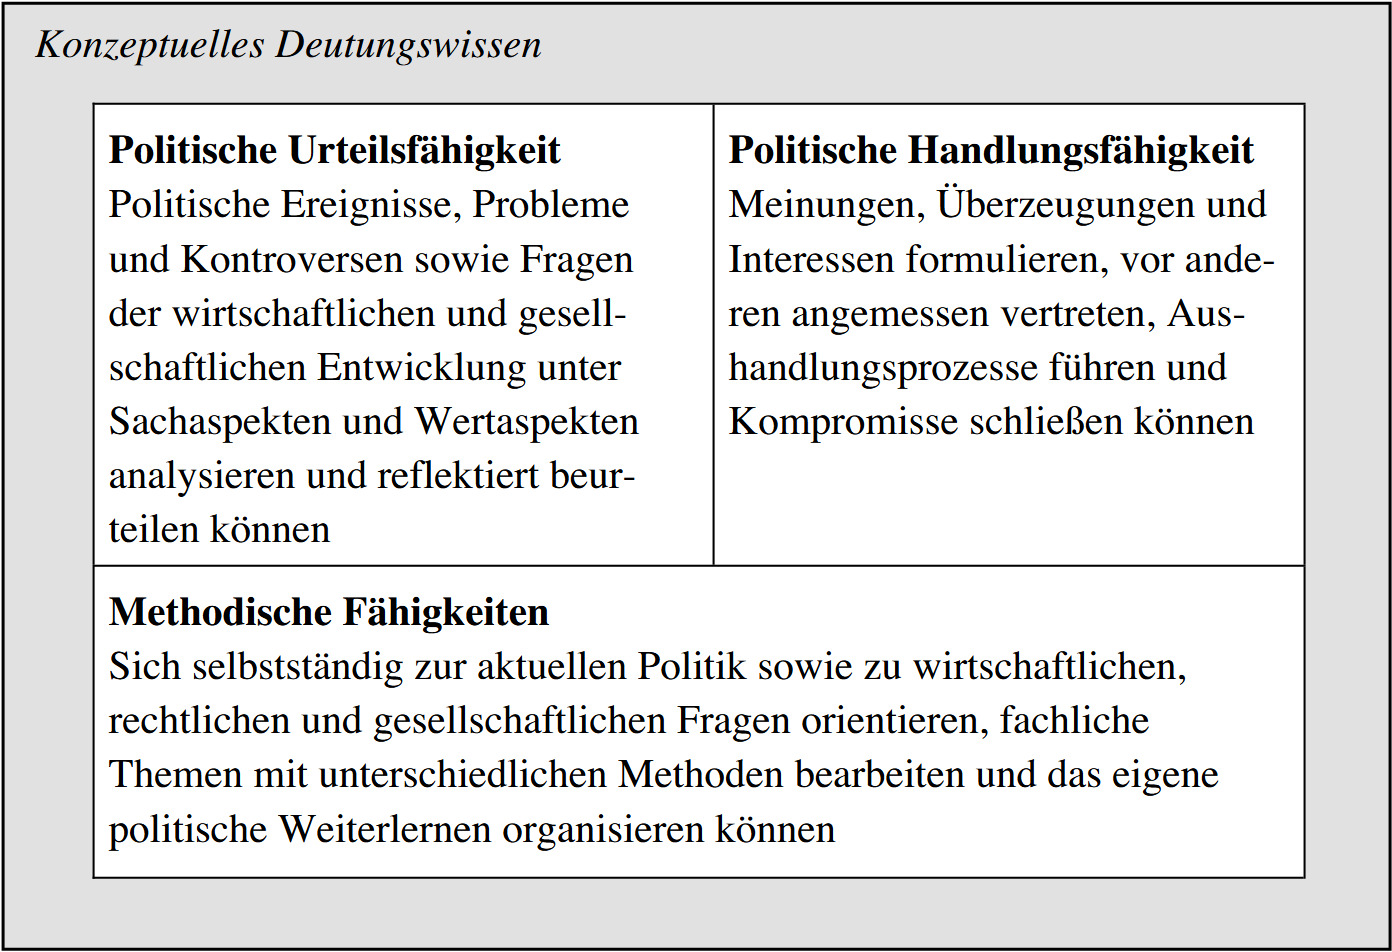
\includegraphics[width=1\linewidth]{gpje 2004 Kompetenzmodell S. 13.png}
    \caption{\enquote{Kompetenzbereiche} der \gls{gpje} \autocite[13]{gpje2004}. Genauso auch im Bildungsplan \autocite[10]{bplan} zu finden.}
    \label{gpjeKompetenzmodell}
\end{figure}

\textcite[106-107]{Gloe2020} skizzieren weiter, wie zu dieser Zeit auch 
\enquote{die eher sozialwissenschaftlich geprägte/n Vertreter[*innen] der Fachdidaktik Günter C. Behrmann, Tilman Grammes, Sibylle Reinhardt und Peter Hampe Kernkompetenzen} der politischen Bildung als fünf \enquote{Demokratie-Kompetenzen} vorschlagen:
\begin{itemize}
    \item Wahrnehmung und Übernahme der Handlungsperspektiven Anderer, auch Dritter, zum Wechsel der eigenen Perspektive, zur Vermittlung des Eigeninteresses mit den Interessen Nah- und Fernstehender und dessen Ausweitung in Richtung auf allgemeinere Interessen (Perspektivenübernahme); 
    \item diskursiven Klärung konkurrierender und konfligierender Ideen und Interessen und zum Aushandeln von Konfliktregelungen und -lösungen (Konfliktfähigkeit); 
    \item problemorientierten Analyse struktureller Bedingungen und institutioneller Ordnungen sozialen, insbesondere politischen und wirtschaftlichen Handelns und zum Gebrauch sozialwissenschaftlicher Begriffe und Methoden (sozialwissenschaftliches Analysieren); 
    \item Einschätzung und Bewertung gesellschaftlicher Problemlagen, politischer Forderungen, Handlungschancen und -alternativen sowie zum reflektierten Gebrauch von Urteilskriterien (politische Urteilsfähigkeit); 
    \item Beteiligung an bürgerschaftlicher Selbstverwaltung, sozialen und politischen Initiativen, innerbetrieblicher und -organisatorischer Mitbestimmung, informellen und formalisierten Prozessen öffentlicher Meinungs- und Willensbildung (Partizipationsfähigkeit/demokratische Handlungskompetenz) 

    (\textcite[337 f.]{Behrmann.2004} \gls{zit} nach \textcite[106-107]{Gloe2020})
\end{itemize}
\citeyear{weißeno.2010} veröffentlichten Georg Weißeno, Joachim Detjen, Ingo Juchler, Peter Massing und Dagmar Richter \citetitle[\emph{Ein Kompetenzmodell}]{weißeno.2010}. Das darin vorgebrachte Kompetenzmodell % (\gls{s} \gls{abb} \ref{2010kompMod}: \gls{S} \pageref{2010kompMod}) 
sorgte für einen neuen Diskussionsanstoß. 
\begin{figure}[htb]
    \centering
    \includegraphics[width=1\linewidth]{Weißeno et al. 2010 p.12.png}
    \caption{\enquote{Basis- und Fachkonzepte der Politik} \autocite[12]{weißeno.2010}}
    \label{2010kompMod}
\end{figure}
Wie in \gls{abb} \ref{2010kompMod} (\gls{S} \pageref{2010kompMod}) zu sehen, sind 30 Fachkonzepte drei Basiskonzepten zugeordnet. Es wird Wert darauf gelegt, mit Schüler*innen-Vorstellungen zu arbeiten. Im Sinne des Konstruktivismus keine abwegige Vorstellung.
An Aussagen wie \enquote{Für erfolgreiches Lernen gilt, dass die Schüler/-innen mit dem in dieser Darstellung vorgestellten Fachvokabular angemessen umgehen können} \autocite[13]{weißeno.2010} lässt sich jedoch Kritik üben. Für die Messung des Outputs ist Fachvokabular sicherlich hilfreich, aber es ist nicht zwingend notwendige Bedingung, um die Wirkungsmechanismen von Macht zu verstehen oder das Zustandekommen von kollektiv verbindlichen Entscheidungen nachvollziehen und beeinflussen zu können -- was womöglich auch Dimensionen von Kompetenzen der politischen Bildung sind. Entsprechend vielfältiger Möglichkeiten Kritik zu üben, skizzieren \textcite[108-109]{Gloe2020} wie sich die Autorengruppe Fachdidaktik\footnote{
    Anja Besand, Tilman Grammes, Reinhold Hedtke, Peter Henkenborg, Dirk Lange, Andreas Petrik, Sibylle Reinhardt und Wolfgang Sander} 
zusammenfand und in ihrem Werk \citetitle{Besand.2011} -- wie der Untertitel \emph{Eine Streitschrift} impliziert -- auch entsprechend Kritik am Modell um \citeauthor{weißeno.2010} üben. 

Auch die Autorengruppe Fachdidaktik hat der Komplexität der Realität folgend eine wortreiche und zahlreich gegliederte Graphik in ihrer Streitschrift abgebildet. Diese ermöglicht einen schnelleren Überblick auf deren vorgeschlagene Einteilung der Kompetenzen der politischen Bildung in Basis- und Fachkonzepte, auch wenn sie keine strengen Vorgaben zur begrifflichen Einteilung geben möchte (\gls{abb} \ref{2011kompMod}: \gls{S} \pageref{2011kompMod}).

\begin{figure}[htb]
    \centering
    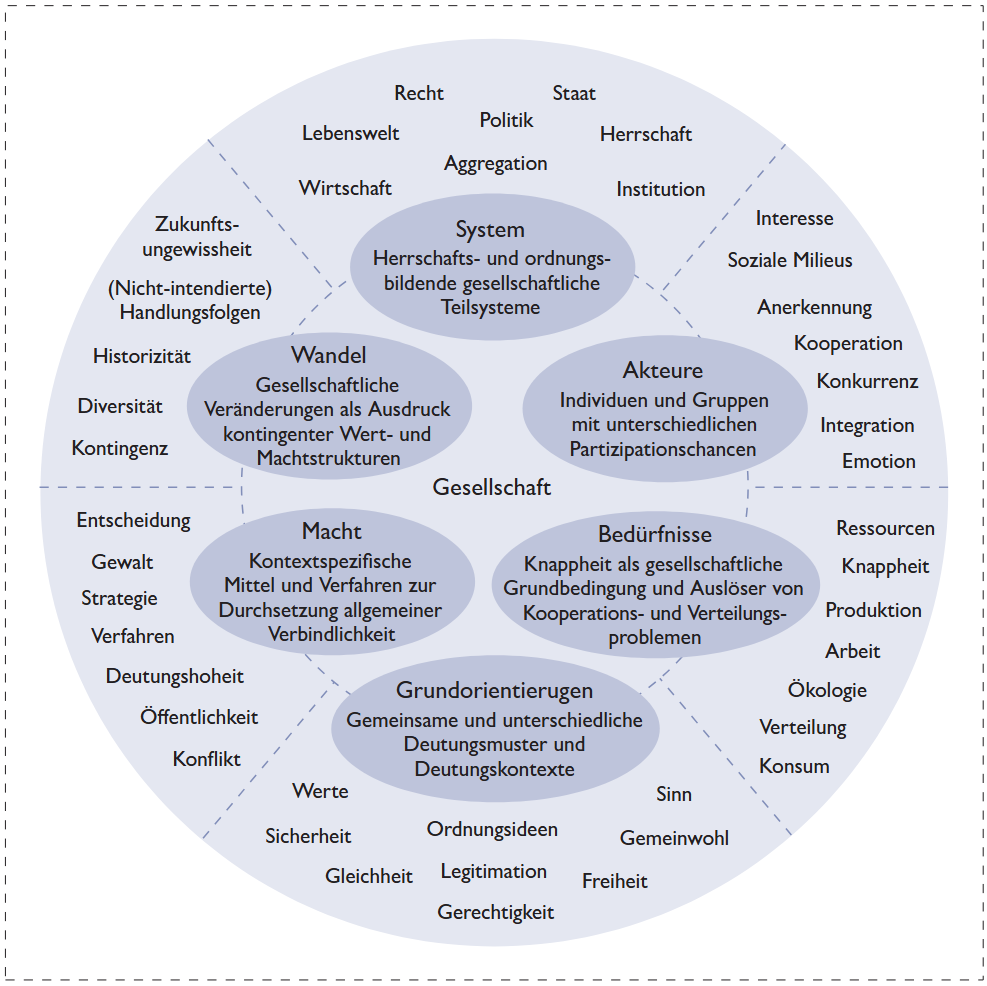
\includegraphics[width=1\linewidth]{Autorengruppe p. 170 nach GloeOeftering p. 109.png}
    \caption{Basis- und Fachkonzepte der politischen Bildung der \\ \textcite[170]{Besand.2011} \gls{zit} nach \textcite[109]{Gloe2020}}
    \label{2011kompMod}
\end{figure}

Der entfachte Diskurs (oder die kontinuierliche (Lohn-)Arbeit der Forschenden?) führte zu einer Art Schlagabtausch\footnote{Was veranlasst an dieser Stelle die Nutzung dieses Wortes und der damit verbundenen schriftlichen Tonalität? \Gls{zb} Die schriftliche Tonalität des Beitrages \citetitle{Massing.2011}: \enquote{Auch zu den Vorschlägen der Autorengruppe Fachdidaktik wird hier nichts gesagt, die ein Teil ihrer Kritik nur wiederholt und deren Alternative bestenfalls den Status einer Ideensammlung hat.} \autocite[135]{Massing.2011}.}, fruchtete aber auch in einem überarbeiteten Modell (\gls{abb} \ref{2012kompMod}: \gls{S} \pageref{2012kompMod}).

\begin{figure}[htb]
    \centering
    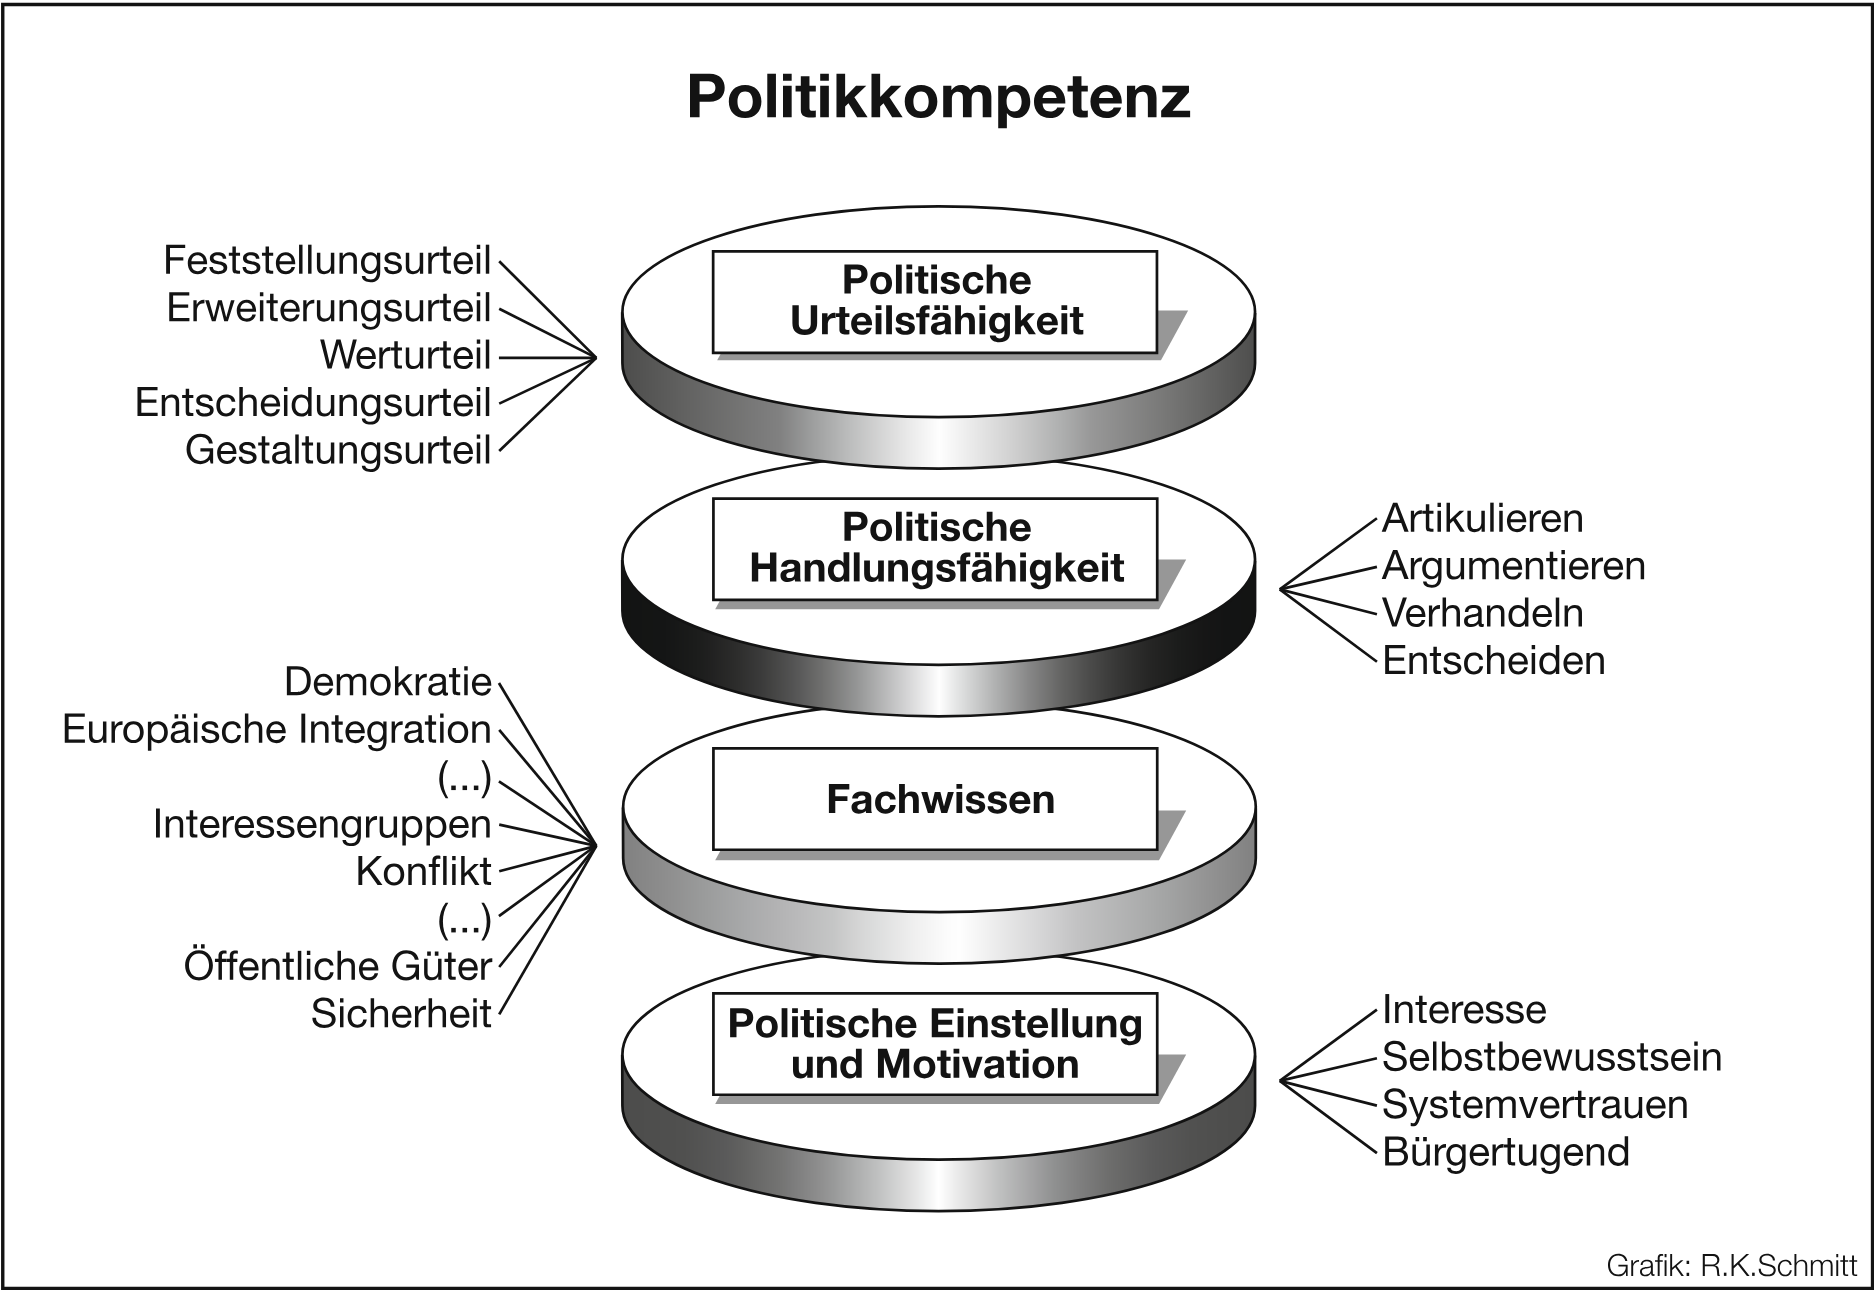
\includegraphics[width=1\linewidth]{Detjen et al. 2012 p. 15.png}
    \caption{\enquote{Modell der Politikkompetenz} \autocite[15]{Detjen.2012}}
    \label{2012kompMod}
\end{figure}

Im Rahmen dieses erneurten Modells, wurde sich weiter abgearbeitet. So führt \textcite[27]{Massing2012} aus, wie \emph{Artikulieren}, \emph{Argumentieren}, \emph{Verhandeln} und \emph{Entscheiden} die \enquote{Kompetenzfacetten} des \emph{kommunikativen-} und \emph{partizipativen politischen Handelns} bilden. 
Insbesondere für das \emph{partizipative politische Handeln} führt \textcite[27]{Massing2012} aus, dass beim \emph{Verhandeln} Machtpotenziale, Konfliktfähigkeit, ökonomische Ressourcen oder Tausch genutzt werden können, um \enquote{Verhandlungsprozesse abzukürzen und zu hierarchisch autoritären oder hierarchisch majoritären Entscheidungen zu gelangen. Diese lassen sich im Unterricht zwar nicht erfahren, sollten aber gewusst werden}. 
Mit einem kreativeren Ansatz ließe sich zwar überlegen, inwiefern \gls{zb} mit einer interdisziplinären Verstrickung mit dem Fach Darstellendes Spiel nicht auch ein ausreichend geschützter Rahmen geschaffen werden kann, in welchem Machtpotenziale durchaus erfahren werden können. Für \emph{Entscheiden} wird jedoch ausgeführt, dass \enquote{Entscheiden durch kooperative oder handlungsorientierte Methoden geübt werden kann}, es aber \enquote{gegenüber der realen Politik unterkomplex} bleibt \autocite[27]{Massing2012}. Diese Kritik bleibt berechtigt und eine ähnlich gelagerte Problemstellung wird in \gls{abs} \ref{fakePartizipation} (\gls{S} \pageref{fakePartizipation}) aufgegriffen. 


% Zum Verhandeln gehören neben argumentativen Strategien, die der konsensuellen Entscheidungsfindung dienen, auch Strategien, die durch den Einsatz von Machtpotenzialen, Konfliktfähigkeit, ökonomischen Ressourcen oder Tausch versuchen, Verhandlungsprozesse abzukürzen und zu hierarchisch autoritären oder hierarchisch majoritären Entscheidungen zu gelangen. Diese lassen sich im Unterricht zwar nicht erfahren, sollten aber gewusst werden. Entscheiden als Teil des realen partizipativen politischen Handelns lässt sich im Unterricht nur begrenzt fördern. Auch wenn Entscheiden durch kooperative oder handlungsorientierte Methoden geübt werden kann, bleibt es gegenüber der realen Politik unterkomplex. Allerdings lassen sich an konkreten politischen Fällen, Problemen, Konflikten oder Entscheidungsprozessen unterschiedliche Strategien und ihre Wirksamkeit analysieren, deren Ergebnisse den Lernenden dann als Fachwissen zur Verfügung stehen. 


%Die Dimensionen sind dabei nicht isoliert, sondern interagieren miteinander, um ein umfassendes Verständnis und eine effektive Handlungskompetenz in politischen Kontexten zu fördern.

Massing stellt diesen Zusammenhang wie ein beleidigter Frosch nicht her\autocite[23]{Massing.2022}




Bei allen Diskursen um die Ausformulierung von Kompetenzen in Worte und zweidimensionale, druckbare Modelle (welche mit Worten wieder das vernetzte, interdependente und quasi dreidimensionale eingebaut bekommen), bleibt mit gewissem Abstand zu erkennen, dass sie sich in weiten Teilen ähneln.
Die einen \autocite{weißeno.2010} hatten den Fokus auf klare und hilfreiche Strukturen gelegt und sind daher das Wagnis eingegangen, sehr konkrete Begrifflichkeiten zu finden. Um als Lehrkraft oder Schüler*in Orientierung zu bekommen, ist das sicherlich hilfreich. Den Anderen \autocite{Besand.2011} war womöglich wichtiger, dass klar wird, dass nicht zwangsweise Fachwissen im Fokus stehen muss, da Zusammenhänge auch ohne die letzten Endes austauschbaren Begriffe verstanden werden können und dieses Verstehen im Vordergrund stehen sollte. 

An welchem Punkt der \gls{bbk} recht deutlich wird und damit auch einen Kern von echter Demokratie trifft, ist die politische Handlungsfähigkeit. In einer pluralistischen Gesellschaft macht es viel Arbeit, wenn alle möglichst gleichen Zugang zu Entscheidungsbeeinflussungen haben sollen. Hilft aber auch dem demokratischen Gedanken. 
Frank \textcite[466]{Nonnenmacher2010} beginnt einen Abschnitt damit, dass bisweilen handlungsorientiert mit schüler*innen-aktivierend gleichgesetzt wird. Von der Wortbedeutung her ist das sicherlich nicht falsch. Aber schon im \gls{bbk} steht man soll \enquote{die vorgefundene politische Lage nach seinen[/ihren] Interessen [...] beeinflussen} lernen (\gls{vgl} \gls{abs} \ref{bbk}: \gls{S} \pageref{bbk}). \textcite[466-467]{Nonnenmacher2010} führt jedoch aus, dass die Debatte aus den 1970er Jahren eher dazu geführt hätte, dass \enquote{das politische Handeln im engeren Sinne -- assoziiert mit Demonstration, Streik und zivilem Ungehorsam -- von vornherein in den Verdacht gestellt wurde und wird, dem bloßen Aktionismus, also einer entrationalisierten und emotionalisierten Geschäftigkeit Vorschub zu leisten}, was dem \emph{Überwältigungsverbot} widersprechen würde.
Bissig bemerkt er wie unentschuldigtes Fehlen bei Demonstrationen zum Bildungsnotstand sanktioniert werden soll, aber wenn \enquote{karitative Bemühungen hinter einer \enquote{Aktion} stehen, ist öffentliches Lob zu erwarten, weil ehrenamtliches soziales Engagement in einer Gesellschaft, die gerade auf diesem Gebiet immer mehr Verantwortung in den privaten Bereich verlagern will, hoch willkommen ist} \autocite[467]{Nonnenmacher2010}.


Er stellt drei Bedingungen, die eingehalten werden sollten, wenn tatsächliche poltische Aktionen in Zusammenhang mit Schule stattfinden sollten:
\begin{enumerate}
    \item Engagement auf \enquote{breiter Wissennsbasis} nach vorhergehender \enquote{Sachanalyse}.
    \item Absoulute Freiwilligkeit für alle Beteileigten. Demnach auch außerhalb der Unterrichtszeit stattfindend.
    \item Öffentlichkeit herstellen. % $\rightarrow$ Das bedeutet 
    
    \autocite[467]{Nonnenmacher2010}
\end{enumerate}


Das mit der sinnvollen Einschränkung der Freiwilligkeit schließt \enquote{echte} poltische Aktionen für das hier untersuchte Material natürlich weitestgehend aus. Aber es ist avon auszugehen, dass es etwas zwischen \enquote{so banale[n] Tätigkeiten wie Lückentexte ausfüllen} \autocite[466]{Nonnenmacher2010} und einer Demonstration mit zivilem Ungehorsam gibt, was Schüler*innen aktivierend ist und auch die Chance bietet politisches Handeln wenigstens zu simulieren. 
\emph{Simulieren} unter anderem, weil \textcite[467]{Nonnenmacher2010} dazu korrekterweise anmerkt, dass Schule eine \enquote{Zwangsveranstaltung} sei. Er geht darauf ein, wie verschiedene Initiativen sich immer wieder darum bemühen Schule zu einem demokratischeren Raum zu machen \autocite[467-469]{Nonnenmacher2010}, kommt jedoch zu einem ernüchternden Schluss, wie insbesondere folgendes Zitat verdeutlicht:
\begin{quote}
    Nichts ist aber an dem Faktum zu ändern, dass diese partizipatorischen Elemente immer nur \enquote{gewährt} werden können; solche Spielräume sind eben wie in allen autoritären Systemen auch jederzeit von den Trägern der Macht wieder zurücknehmbar. 

    \autocite[468]{Nonnenmacher2010}
\end{quote}




\subsection{Bildungsplan für berufsbildende Schulen oder allgemeine politische Bildung mit Zielgruppenorientierung?}
% Politik an berufsbildenden Schulen in Bremen wird neben Deutsch als einziges Fach für alle Fachrichtungen berufsübergreifend unterrichtet. 
Daher findet sich strukturell wenig Unterscheidung zu dem Fach Politik an allgemeinbildenden Schulen.
Der Bremer Bildungsplan für Politik in der Berufsbildung ist mit der Veröffentlichung 2023 auch wesentlich aktueller als die Bildungspläne welche Politik beinhalten von 2006, 2008 und 2010 für die allgemeinbildenden Schulen in Bremen. 
Mit der Arbeitnehmerkammer Bremen wird sich außerdem auf einen lokalen Akteur bezogen, welcher voraussichtlich auch für einen Großteil der Bremer Schüler:innen an allgemeinbildenden Schulen relevant werden könnte. 
Zumal die politische Bildung an Berufsschulen sich explizit nicht auf den beruflichen Bereich beschränken soll, sondern gesamtgesellschaftliche Zusammenhänge zum Thema hat. Genau wie an allgemeinbildenden Schulen und bei politischer Bildung im Allgemeinen.

% Politische Bildung ist (oder sollte) in zahlreichen Lebensbereichen verortet (sein). Daher sei auf das Offensichtliche hingewiesen. Es handelt sich hier um Unterrichtsmaterial, welches für die staatlich institutionalisierte Bildung eingesetzt werden soll. 
% Dieses Bildungsmaterial soll jedoch mit einem anderen staatlichen Akteur herausgegeben werden. 

Wie werden Demokratiekompetenzen gefördert? Wird Wissen über Demokratiekompetenzen gefördert oder gar direkt demokratisches oder eben undemokratisches Handeln erprobt und reflektiert?


\subsection{Sozioökonomische Bildung, politische Bildung und interdisziplinäres Begriffs Wirrwarr \label{polBildung}}

Politische Bildung % im Kontext staatlicher Bildungsakteure 
ist im Schulkontext häufig nicht nur im Fach Politik, Sozial- oder Gemeinschaftskunde verortet, sondern auch häufig in Fächern mit Bezeichnungen, in denen \enquote{Politik} gleichbedeutend neben \enquote{Wirtschaft} genannt wird. 
So finden sich im Sachstandsbericht der Wissenschaftlichen Dienste des Deutschen Bundestags (\citeyear[5]{WD8.2016}) Fächerbezeichnungen wie \enquote{Politik / Gesellschaft / Wirtschaft} für Hamburg, \enquote{Politik und Wirtschaft}, \enquote{Politik-Wirtschaft} \& \enquote{Wirtschaft/Politik} in Hessen, Niedersachsen und Schleswig-Holstein oder \enquote{Gemeinschaftskunde / Rechtserziehung / Wirtschaft} für Sachsen. Damit ist in 5 von 16 Bundesländern politische Bildung schon in der Fächerbezeichnung an Wirtschaft gekoppelt \autocite[vgl. zu der tatsächlichen Zeit, die für politische Bildung im Unterricht an allgemeinbildenden Schulen zur Verfügung steht auch][14 \& 16]{Gokbudak2020}.

Materielle Bedingungen in der Sphäre des Politischen sind nicht von der Hand zu weisen. Die Beschäftigung mit materiellen Verhältnissen in der politischen Bildung respektive mit Wirtschaft ist also naturgegeben.
Als Forschungsfeld wird daher gerne auch von Sozioökonomischer Bildung gesprochen.
Insbesondere zu diesem Begriff lässt sich Forschung zu Unterrichtsmaterial und Einflussnahme externer Akteur*innen finden.


Die Bezeichnungen sowohl von Forschungsdisziplinen als auch von Schulfächern, versuchen dieser interdisziplinären Verknüpfung mal mehr, mal weniger gerecht zu werden.
Da die Trennschärfe solcher Begriffe Gefahr läuft, eine philosophische und linguistische Debatte über die Unzulänglichkeiten von Sprache zu eröffnen, wird in dieser Arbeit stets versucht, ein nach Ansicht des Autors möglichst passenden Begriff für den gerade gemeinten Gegenstand zu nutzen, welcher aber explizit nicht beansprucht, dass andere Begriffe aus leicht verändertem Blickwinkel nicht ebenso passend wären und lediglich eine notwendige Entscheidung darstellt. 

% Der Begriff Politik Wirtschaft ist dabei 


Als Tatsache kann angesehen werden, dass sich Gesellschaft und Kultur mit Wirtschaft wechselseitig beeinflussen. 


\subsection{Arbeitnehmerkammer Bremen (ANK)}
Im Gesetz über die Arbeitnehmerkammer im Lande Bremen \autocite[]{ArbnkG} ist festgesetzt, dass nach der Beitragsordnung \autocite[]{ArbnkB} Beiträge nahezu aller Arbeitnehmenden\footnote{ 
Auf der Lohnabrechnung für einen Minijob taucht \gls{zb} kein Abzug für die \gls{ank} auf. Dies orientiert sich an der Geringfügigkeitsgrenze, welche für 2025 556€ beträgt \autocites{b.gering}{banz.gering}.} in Bremen zu erheben sind. Systemisch ähnlich zu Steuerzahlungen ist die Mitgliedschaft in der Kammer daher mit Zwangsbeiträgen verbunden. 

Im Gesetz zur \gls{ank} ist in \S2(1) \autocite[1]{ArbnkG} zu den Aufgaben der Kammer unter anderem formuliert: \enquote{Maßnahmen zur Förderung und Durchführung der beruflichen sowie der allgemeinen und politischen Weiterbildung der Kammerzugehörigen zu treffen}.


Da die \gls{ank}, wie der Name schon vermittelt, durchaus partikulare Interessen der Arbeitnehmer*innen vertritt, 



\subsection{Medienkompetenz und die unbedingte Verknüpfung zu \enquote{Wahrheit} \label{media}} 

\subsection{\enquote{Wahrheit}, \enquote{Wahrhaftigkeit} und \enquote{Richtigkeit} \label{wahr}}

Für die Argumentation im Abschnitt der Medienkompetenz (\gls{abs} \ref{media}: \gls{S} \pageref{media}) ist eine Begriffsdefinition der drei Begriffe aus der Überschrift hilfreich. Da diverse Kompetenzmodelle der politischen Bildung auch die politische Handlungsfähigkeit als Ziel attestieren und zu dieser auch Meinungsbildung und -durchsetzung gehört, ist es praktisch, dass diese Begriffe im Rahmen eines Kommentars zu dem Begriff Meinung dargestellt werden\footnote{Der folgende Abschnitt ist übernommen aus einer Hausarbeit von \textcite[4]{Klein2022}}:

In dem Essay \enquote{Bloße Meinung} beobachtet Frank \textcite[]{Nullmeier2019} kritisch, wie als Reaktion auf Desinformation eine absolute Wissenschaftlichkeit gefordert wird, welche die Meinung mit einem Anspruch auf Wahrheit \enquote{auf die Seite des zu Verwerfenden} \autocite{Nullmeier2019} stellt.  Weiterhin bezieht Nullmeier sich auf drei Begriffe für Wahrheit:
\begin{enumerate}
    \item Wahrheit: Als Wahrheit empirischer Aussagen.
    \item Wahrhaftigkeit: Als Begriff um mit Unwahrhaftigkeit die Lüge kennzeichnen zu können - In der Abgrenzung zu Unwissen oder sich als falsch erweisenden empirischen Wahrheit. In der Lüge ist die Wahrheit enthalten, sie wird nur nicht gesagt. 
    \item Richtigkeit: Als Begriff, um eine Wahrheit für normative Aussagen zu haben, die sich aus \enquote{eine[r] partiell wahrheitsanaloge[n] Logik der Argumentation mit der Annahme einer aus richtig und falsch bestehenden Binarität und einer potenziell allein richtigen Aussage [er]geben} \autocite{Nullmeier2019}.
\end{enumerate}

Er führt aus, dass Meinung in demokratischen, politischen Entscheidungsprozessen von einer immanenten Wichtigkeit ist. Entsprechend wichtig sollte die Meinung daher auch im Politikunterricht sein.


Medienkompetenz sollte in allen Fächern der Schule grundsätzlich, aber aufgrund der großen Schnittmenge insbesondere im Politikunterricht mitgedacht und mitgemacht werden. 
Noch konkreter argumentiert: Medienkompetenz ist lediglich ein bestimmte Bereiche betonender Begriff für integrale Lerngegenstände von politischer Bildung. Diese Lerngegenstände ergeben sich aus der Zielsetzung der geforderten Kompetenzen. Eine konkrete und praktische Umsetzung von Medienkompetenz kann dabei in Quellenarbeit und Zitation gesehen werden.
 
\subsubsection{Die Zerteilung der Welt durch Worte}
Daher nun ein kleiner philosophischer Ausbruch in die Verknüpftheit von Wissen und Sprache: Auch in dem Entstehungszeitraum der vorliegenden Arbeit sind \enquote{Wahrheit}, \enquote{Wahrhaftigkeit} und \enquote{Richtigkeit} nicht nur in der Kommunikation grundsätzlich, sondern insbesondere auch im Politischen eine zentrale Debatte. 
Im Zeitalter von Desinformation, \enquote{framing}, Populismus und Propaganda ist für die Erziehung zu mündige(re)n Menschen die Auseinandersetzung mit der Produktion von Wissen und \enquote{Wahrheit} unerlässlich. Die im vorigen Satz aufgezählten Begriffe enthalten immer eine Form \enquote{Unwahrhaftigkeit} oder das (teils bewusste) Auslassen von \enquote{Wahrheit}. Um die verschiedenen Formen und Unterschiede des Irrens und der Lüge durchdringen zu können, ist entsprechend ein Anschneiden dieses Themenkomplexes unerlässlich.  

Über das bloße, eher oberflächliche, Verstehen von Inhalt selbst hinausgehend, ist ein wesentlicher Bestandteil von Medienkompetenz, den Inhalt bewerten zu können. In diesem Zusammenhang soll bewerten bedeuten, den Inhalt mit anderen Dingen zu verknüpfen. Denn da Wissen (oder \enquote{Wahrheit}) grundsätzlich in Beziehung von Subjekten zur Welt und Beziehung untereinander erschaffen wird, ist es geradezu unabdingbarer Bestandteil eines verstehenden Wissenserwerbs, das Wissen auch mit dem Kontext, in welchem es entstanden ist, zu verknüpfen. Das Verknüpfen von Wissen ist dementsprechend auch Voraussetzung für ein tiefergehendes Verstehen. 

Die Diskussion, inwiefern Wissen auf Logik basierend auch mit wenig Beziehung zu anderen Subjekten und der dinglichen Welt \enquote{erschaffen} oder \enquote{erkannt} werden kann, soll an dieser Stelle ausgeklammert werden. Denn pragmatisch gesehen ist jede Form von Information in der physischen Welt mindestens als Energiezustand verankert. Menschen lernen das Denken insbesondere an ihren über die Sinnesorgane vermittelten Erfahrungen mit der dinglichen Welt, was dann erst mit der Zeit höhere Abstraktionsebenen (Symbole, Sprache, Wittgenstein \gls{etc} gib' ihm) ermöglicht. Und auch noch so stark abstrahierte Informationen sind eben immer noch mindestens irgendwie messbar in der physischen Welt verankert. Sei es eine Schallwelle des gesprochenen Wortes, eine neuronale Verbindung im Gehirn, Spannung oder Magneten in einem Computer, Symbole auf Papier oder spezifisch angeordnete Basentriplets einer messengerRNA auf dem Weg, ein Protein synthetisieren zu lassen. 

Ein eingängiges Beispiel für die unbedingte Verknüpftheit von Wissen lässt sich am Wort \enquote{Baum} darstellen. Erstens muss -- um dem Wort eine über den Zufall hinausgehende Bedeutung zu verleihen -- mindestens irgendein Subjekt das Wort tatsächlich mit einem Konzept von Baum verknüpfen. Wenn Sprache ihre Funktion der Kommunikation -- unter der wir sie kennen -- erfüllen soll, am besten mehrere Subjekte.
Ferner könnte ein Baum nicht existieren ohne Wasser, die Energie der Sonne, Jahrmillionen an Evolution, Erde \gls{etc} Sprache zerlegt eine zwangsläufig verknüpfte Welt immer in Bestandteile. 
Wer das Konzept (also das Wort und das Wissen, welches es bezeichnet) \enquote{Baum} verstehen möchte, weiß in irgendeiner Form auch Teile dieses zwangsläufigen verknüpften Wissens. Denn um das Wort \enquote{Baum} gebrauchen zu können, wird der Baum von der Sonne und aus der Erde herausgetrennt. Wenn das nicht so wäre, gäbe es keine Worte. Weil konsequent zu Ende gedacht immer nur ALLES ausgedrückt werden könnte, da über genügend Umwege alles miteinander verknüpft ist. 

\vspace{12pt}
\hrule
\vspace{12pt}

back to it


\subsubsection{Quellen}

An diese Quellendarstellungen muss sich im Sinne der didaktischen Reduktion jetzt nicht sklavisch gehalten werden.
Als polemisches Beispiel: Im Mathematikunterricht in der Elementarstufe bedarf es womöglich zu viel mental load, um auf die Verschriftlichungen von Adam Ries Bezug zu nehmen. Aber vom Grundsatz her ist es durchaus angebracht, so viel Quellenmaterial wie möglich, so präzise wie möglich auch im Unterrichtsmaterial selbst mitanzugeben. Alleine um mit gutem Beispiel voranzugehen. 
% Diggah, mach halt immer ehrenloses Scheißquellengeballer, anstatt Infos gehaltloser rauszuballern als gmx.de newsflash. Medienkompetenz ist Sack, die Medienlandschaft und Lehrmaterial sind aber auch häufig genug beschämendes Negativbeispiel. Jeder Scheiß Porno hat mit seinen blöden Wasserzeichen mehr Qualität in der Nachverfolgbarkeit der Urheberschaft. Man


Eine gute Vorbildfunktion ist essentielle Voraussetzung für verschiedene Formen des Lernens, wie es theoretisiert wird.
Egal, ob es sich um das Beobachtungslernen \autocite[73ff.]{Kiesel2012} welches maßgeblich von Albert Bandura definiert wurde, handelt, oder ob im Rahmen des (zwar umstrittenen) impliziten Lernens \autocite[83ff.]{Kiesel2012} stattfindet. Ohne ein auch positiv-Beispiel zu haben, wird das Erlernen von der Relevanz und der methodischen Durchführungsmöglichkeiten einer guten Quellenarbeit erschwert. Aus dem Grunde ist der Bildungsbereich von Beginn an gut beraten, stets gute Beispiele für die Quellenarbeit darzustellen. 


Darüber hinaus Einstellung \autocite[130]{Kiesel2012}



\subsection{Zielgruppe}
Gutes Unterrichtsmaterial ist nicht per se gut, sondern es ist lediglich abhängig von den Rezipient*innen gut. Eine womöglich gut vorbereitete Lerneinheit zu Polynomdivision für Studierende in Höherer Mathematik ist in einer Elementarstufe, die gerade überhaupt dividieren lernt, sicherlich nicht mehr gut. Gutes Unterrichtsmaterial ist also in erster Linie für die intendierte Zielgruppe zu untersuchen. Jede Lerngruppe ist individuell, dennoch lässt sich allein durch das Alter, den Lernort und -- zum Teil  mit dem Ort einhergehend -- die Sprache und viele weitere Faktoren, die Lerngruppe bereits stark abgrenzen. Genau das passiert auch bei einem Englischbuch, welches für Unterricht auf Deutsch in der 5./6. Klasse in Baden-Württemberg veröffentlicht ist. 

Es ist also angezeigt, die Zielgruppe des Unterrichts möglichst klar abzugrenzen, wenn untersucht werden soll, ob Material \enquote{gut} ist. 


Wenn es dann genauer an die Planung von konkretem Unterricht geht, sind insbesondere die Lehrpersonen gefordert, um auf den Wissensstand und bestehende Schüler*innen-Vorstellungen eingehen zu können. Nach dem Modell der didaktischen Rekonstruktion sollen Lerninhalte besser und nachhaltiger vermittelt werden, wenn dies geschieht \autocite[404-406]{Reinfried2009}.

Dadurch, dass das Material mit Fokus auf duale Studiengänge berufsbildende Schulen erstellt ist, unterscheidet sich die Zielgruppe von der an allgemeinbildenden Schulen in dem wesentlichen Punkt, dass gerade der Lebensweltbezug für Arbeitsthemen durch die eigenen Arbeitserfahrungen im Betrieb deutlich weniger theoretisch ist, als wenn an einer Oberschule zum Beispiel über Arbeitsschutz gesprochen wird. 

\enquote{Fremdzuschreibungen und defizitorientierte Ansprachen von Personengruppen sind deshalb problematisch, weil sie die in unserer Gesellschaft ungleich verteilten Zugänge zu u.a. Bildung und Chancen mitunter eher reproduzieren als sie – wie von einer inklusiven politischen Bildung} \autocite[]{Beckmann2022}
Dennoch ist es wichtig, die Zielgruppe zu kennen und darauf einzugehen.



2024-12-11
Wie wird die Zielgruppe angesprochen?
Wird eine heterogene Zielgruppe angesprochen?
Bla über Defizitorientierung
% https://profession-politischebildung.de/grundlagen/grundbegriffe/defizitorientierung/#:~:text=Defizitorientierung%20meint%20die%20Fokussierung%20auf,Bildungsangeboten%20sowie%20im%20p%C3%A4dagogischen%20Handeln.
% die website zitiert z.B: bei Citavi Holzer 2010

\subsubsection{Schüler*innenvorstellungen}
Nach dem Modell der didaktischen Rekonstruktion \autocite[]{Reinfried2009} ist die Inbezugnahme von Schüler*innenvorstellungen ein zentrales Element für besseren Unterricht.
Es soll also untersucht werden, an welchen Stellen das Material Schüler*innenvorstellungen aufgreift oder immerhin Raum dafür lässt. 

\subsection{Was sagt die Wissenschaft zu politischer Bildung an (Berufs)schulen?}
Anja Besand

Reinhold Hedtke (den habe ich schon)

Bettina Zurstrassen (Herausgeberin Sammelband von der bpb) 

Christine Engartner



Die \gls{ank} als Gegenspieler zu wirtschaftsnahem Material? Engartner 2023:7

\subsection{Ökonomische versus politische Sozialisation?}
In der Forschung zu politischer Bildung in staatlichen Institutionen wird seit geraumer Zeit verhandelt, wie die Einflussnahme externer Akteure zu bewerten sei. Reinhold Hedtke 

Autor*innen, welche einen bildungstheoretischen und/oder einen politikwissenschaftlichen Hintergrund aufweisen, lesen sich insofern ähnlich, als dass ihnen gemein ist eine gute politische Bildung interdisziplinär zu gestalten. Insbesondere für den berufsbildenden Bereich lässt sich feststellen, dass Forderungen erwachsen, die \enquote{betriebswirtschaftlichen Verwertungslogiken}

dritte Säule \autocite[]{kerschensteiner1966}
% Diggah, wie soll ich Forschungsüberblick geben, wenn alleine Reinhold Hedtke gefühlt gut 200 Veröffentlichungen zur gleichen schmackhaften Soße hat?


\subsection{Mehr Platz für Emotionalität}
Gutes Unterrichtsmaterial gibt die Beziehungsebene zwischen Lehrer*innen und Schüler*innen nicht vor, aber sorgt im Idealfall durch gute Strukturierung und guten Umgang mit den bestehenden Ressourcen dafür, dass die Beziehungsebene mehr Platz bekommen kann.

Gleichzeitig sind Emotionen integraler Bestandteil des Politischen \autocite{Heidenreich.2012a} und sind daher nicht in einem veralteten Dualismus (der Rationalität unverbunden und moralisch unterlegen) aus dem Unterricht zu verbannen. % Auch wenn in dieser Hinsicht noch reichlich Nachholbedarf besteht. 

Dass Emotionen gerade in Zusammenhang mit Politik bisweilen einen faden Beigeschmack haben, trägt Hendrik Schröder (\citeyear[4-5]{Schroder.2020}) 



\subsection{Veröffentlichungsreichweite, Auffindbarkeit, Preis, Einsetzungsreichweite \label{öffi}}

Es darf davon geträumt werden, Unterrichtsmaterial, welches durch öffentliche oder fast öffentliche Gelder finanziert wurde, auch der Öffentlichkeit zugänglich ist.

\subsection{Forschungsfrage}
Wie lässt sich das Unterrichtsmaterial der Arbeitnehmerkammer Bremen bewerten?

Wie und nach welchen Maßstäben lässt sich das Unterrichtsmaterial der Arbeitnehmerkammer Bremen bewerten?

\section{Analysemaßstab}
Analyse

Im Sachunterricht in der Elementarstufe wird kritisiert, wenn der Unterricht wenig mit der eigentlichen Sache zu tun hat \autocite[2-4]{Scholz2004}. Im Politikunterricht ist das Anschauen jedoch weniger auf Dinge bezogen. Analog dazu lässt sich jedoch die bereits im \gls{bbk} geforderte Handlungskompetenz sehen. Spannend ist es also zu untersuchen, inwiefern durch das Material politisches Handeln beobachtbar oder gar an der eigenen Gruppe erlebbar wird.




Einen Teil wird immer eine Fehlerprüfung einnehmen. 

\subsection{Fragen an das Material} % Nach welchen Maßstäben Unterrichtsmaterial analysieren?
Ein eher offen formulierter Bildungsplan ist kein Zufall. % Aus ähnlichen Gründen, die einen offen formulierten Bildungsplan nahelegen,
Daher wäre es kontraindiziert, Unterrichtsmaterial nach starren Vorgaben zu bewerten.
Dennoch soll eingegrenzt werden, nach welchen Maßstäben Unterrichtsmaterial bewertet werden könnte. Offen bedeutet nicht beliebig.

Die erste Anlaufstelle dafür ist der Bildungsplan selbst. In Anlehnung an die Gliederung des Bildungsplans kann das Unterrichtsmaterial anhand folgender Punkte untersucht werden:
\begin{itemize} 
    \item Kompetenzen jeweils der beruflichen \& politischen Bildung
    \item Lebensweltorientierungen % Modell der didaktischen Rekonstruktion
    \begin{itemize}
        \item Arbeits-,  Berufs- und Lebensweltorientierungen
        \item Problem-, und Wissenschaftsorientierungen
        \item Zukunfts-, Gegenwarts- und Vergangenheitsorientierungen
    \end{itemize}
    \item Methodische Grundsätze
    \item Und anhand folgender sieben politischen Handlungsfelder:
    \begin{itemize}
        \item Demokratie 
        \item Gesellschaft 
        \item Arbeitsleben
        \item Öffentlichkeit im digitalen Zeitalter
        \item Wirtschaftspolitik
        \item Globale Zusammenhänge 
        \item Nachhaltigkeit 
    \end{itemize}
\end{itemize}


Im Bildungsplan sind die drei wichtigsten Kompetenzen in Anlehnung an den \gls{bbk} formuliert. 

\begin{itemize}
    \item Politische Urteilsfähigkeit
    \item Politische Handlungsfähigkeit
    \item Methodische Fähigkeiten 
\end{itemize}

Daher soll im nächsten Schritt analysiert werden, inwieweit das Unterrichtsmaterial diese Kompetenzen fördert. 

% Maßgeblich dafür können Vergleiche zu Bewertungskriterien sein, die bereits von anderen genutzt worden sind.
% Auch maßgeblich soll sein, inwiefern schon das Unterrichtsmaterial in Bezug auf den Bildungsplan und dessen, unter Anderem aus dem \gls{bbk} abgeleiteten, Kriterien vereinbar scheint. 


Fragen, die darüber hinaus und ergänzend an das Material gestellt werden sollen, sind:
\begin{itemize}
    \item Welche Kompetenzen werden an welcher Stelle gefördert?
    \item Wie und durch welche Operationalisierung werden die Kompetenzen gefördert?
    \item Wie werden Schüler*innenvorstellungen berücksichtigt? % zB diametral entgegen falscher Vorstellungen oder auf richtige Vorstellungen aufbauend? Außerdem: Stichwort: Reifizierung \autocite[]{Reinfried2009}
    Siehe auch die reflexiven Fragen für das Modell der didaktischen Rekonstruktion bei \textcite[411-412]{Reinfried2009}.
    \item An welchen Stellen soll induktiv, an welchen deduktiv vorgegangen werden?
    \item Ist das im Modell der Didaktischen Rekonstruktion sinnvoll? \autocite[]{Reinfried2009} Sollte im Sinne des Konstruktivismus besonders induktives Vorgehen seitens der SuS antizipiert werden?
    \item Wie wird Schüler*innenaktivität erzeugt? % Für Konstruktivismus wichtig
    \item Wird bestehendes Material benutzt und analysiert oder wird auch eigene Produktion angeregt?
    \item Wie ist die Ergebnissicherung eingebunden?
    \item Welche Handlungsfelder werden angesprochen?
    \item Inwieweit bietet ist das Material auf die Lebensrealität und realistische Partizipationsmöglichkeiten ausgerichtet?
    \item Inwieweit impliziert das Material politisches Handeln, welches bestehende Systeme in Frage stellt? Ist das noch vertretbar (im Konkreten: mit dem \gls{bbk} vereinbar)? Ist im Gegenzug ein Weglassen solcher Perspektiven vertretbar (im Konkreten: mit dem \gls{bbk} vereinbar)?
    \item Welche Medien werden eingesetzt? Wie ist die Wahl der Medien begründet?
    \item Medienkompetenz % siehe Demokratie ANK Dinger Kommentare für die Quellen \emph{M1} und \emph{M2} letzte Seite
    \item Inklusion
    \item Digitalisierung (Methodenkompetenz. Sinnvoll eingesetzt?)
    \item Was wird vom Material an Möglichkeiten der Binnendifferenzierung geboten?
    \item Wo findet eine Binnendifferenzierung statt; sowohl im Inhalt als auch den Methoden? Ist die Wahl der Methoden aus der Didaktik zu begründen? Welche alternative Methoden wären möglich gewesen? Werden unterschiedliche Methoden für unterschiedliche Lerngruppen Angeboten?
    \item Handhabbarkeit, Anwendbarkeit, praktisches, pragmatisch. Handwerkliche Betrachtung
    \item Umfang, Zeitvorgaben, zur Verfügung Stellung realistisch?
    \item Unwahrscheinlich: Aber, ist das Material Altersgruppen geeignet oder gar übergriffig?
    \item Welche Beeinflussungen sind zu erkennen? Lassen die sich diese legitimieren?
\end{itemize}
Darüber hinaus soll untersucht werden, inwieweit sich Intentionen der Arbeitnehmerkammer Bremen im Material finden lassen und ob die Beeinflussungen des Akteurs sich in einem Rahmen bewegen, welcher der Intention des \gls{bbk} nicht entgegensteht. \#Kontroversitätsgebot 


\subsection{Bildungsplan als Analysemaßstab}
Der Bildungsplan \autocite{bplan} in Politik für duale Studiengänge im Land Bremen...

Wie zu Kapitelanfang angedeutet ist der Bildungsplan vergleichsweise offen formuliert, ohne detaillierte Vorgaben zu machen. Angesichts der überbordenden Themenauswahl und interdisziplinären Verstrickung eines Faches wie Politik eine konsequente Entscheidung, die im Bildungsplan selbst argumentativ legitimiert wird \autocite[diggah, welche Seite habe ich das gelesen]{bplan}. Reinhold \textcite[17-18]{Hedtke2016} kritisiert für den Wirtschaftsunterricht den fehlenden Bezug auf die Fachwissenschaften sowie auch eine fehlende Berücksichtigung der zahlreichen Interdependenzen zu benachbarten Fachwissenschaften. 


\subsubsection{MUSS WOANDERS HIN}
AAAAnderes Kapitel
Es wird keine Begründung zur didaktischen Auswahl der Themen mitgeliefert. Damit einhergehend wird auch eine didaktische Reduktion nicht begründet. In der Schulpraxis ist das in explizit schriflticher Form sicherlich auch nicht üblich. In der Ausbildung von Lehrkräften ist genau das jedoch gefordert und es wird implizit erwartet, dass auch später stets eine solide Begründung geliefert werden könnte.
Das Material hat die Intention hat verbreitet und genutzt zu werden. Daher wäre es durchaus eine Überlegung wert, inwieweit es die Legitimation  erhöhen könnte, noch tiefer in die Entscheidungsbegründung einzustiegen.

\subsubsection{MUSS AUCH WOANDERS HIN}
Strukturelle Ähnichkeiten fallen zu dem im Bildungsplan geforderten Verständnis der Möglichkeiten und Grenzen des Föderalismus und folgenden Überlegungen zu Unterrichtsmaterial grundsätzlich auf.
In einem vorstellbaren Ideal, wird eine offene Plattform für die Bereitstelleung von Unterrichtsmaterial bereitgestellt.
Diese sollte mehrere Voraussetzungen erfüllen:
\begin{itemize}
    \item offen in Form von kostenfrei, öffentlich \gls{vgl} \gls{abs} \ref{lizenz}: \gls{S} \pageref{lizenz}f
    \item Das würde bedeuten, es sollte gepusht werden, dass das Ding bestenfalls weltweit -- aber um der Egozentrik der politics Sphäre gerecht zu werden vielleicht erstmal als europaweit beworben -- genutzt wird und nicht jedes Bundesland rumknausert und die gleiche Software $\geq$ 16 mal in Auftrag gibt.
    \item Das aus öffentlichen Geldern finanzierte Ding würde damit auch der Öffentlichkeit gehören und es würden nicht hauptsächlich privatwirtschaftliche Akteure davon profitieren, die die Rechte an ihrem schlechten Produkt halten, bei welchem auch niemand eine realistische Chance hätte es zu verbessen.
    \item Daraus folt $\rightarrow$ Die Plattform sollte als veränderbar angelegt sein.
    \item Das Material sollte von allen veränderbar sein. Was explizit nicht heißen muss, dass jede schlechte oder gar destruktive Änderung gesichtet oder gar übernommen werden muss.
    (Womöglich ist hier such etwas in Richtung Klarnamen-Registrierungszwang angebracht. Hier sollte sich viel aus der Softwareentwicklung abgeschaut werden. Da steckt die Expertise)
    \item Es sollte einen Versionverlauf haben.
    \item Abstimmungsmöglichkeiten sollten gegeben sein. Dann hat man als womöglich staatlich veratnwortliche Person einen Überblick, was ein Ausschnitt der Öffentlichkeit zu dem Ding denkt.
    \item Im besten Falle verschieden filterbare Bewertungsskalen. \Gls{zb} nach Lehrkräfte, Schüler*innen, andere Externe, Herkunftsorte, Alter etc.
    \item 
    \item Überraschung, ich habe extra \emph{Ding} geschrieben. Weil das ziemlich ersetzbar für viele (informationslastige) Produkte ist, welche mit öffentlichen Ressourcen realisiert werden.
    \item diggah, als ob, ich habe kein bock mehr. es wird eh schlimmer anstatt besser
\end{itemize}


Programmierende Freunde von mir scherzen über \emph{pull requests} über \enquote{git} für eine Möglichkeit moderne, digitale Möglichkeiten für direktere Formen der Demokratie nutzen zu können.





\subsection{Politische Bildung in der Fachliteratur -- Ein Auszug}
Im Bremer Schulsystem werden in der Mittelstufe klassische Schulfächer wie Chemie, Physik und Biologie gemeinsam im Fach \gls{nw} \autocite{vogel2010nw} oder im sozialwissenschaftlichen Bereich wurden Geschichte, Politik und Geographie zu meiner Zeit an der Gesamtschule als \gls{wuk} \autocite{vogel2006gs} oder heutzutage an Oberschulen als \gls{gp} \autocite{vogel2010gp} unterrichtet.
% GEHT DIE ICH FORM??
->
Autor:innnen haben auch keinen Bock mehr auf monodisziplinär. 

Die \gls{bpb} hat den Sammelband veröffentlicht.
\subsection{Quellenangaben}
\begin{itemize}
    \item Wie lässt sich die Qualität der Quellen bewerten?
    \item Wie wird auf Medienkompetenz eingegangen?
 \end{itemize}




\section{Analyse der Unterrichtsvorschläge \label{Analyse}}
\paragraph{Hinweis}
Das Material befindet sich in der Entwicklung ist und noch nicht veröffentlicht. Es unterliegt daher noch zahlreichen Veränderungsoptionen. 
Ein besipelhaftes Layout der Materialkarten ist im Appendix auf \acrlong{S} \pageref{ANKPrototyp} zu sehen. Dahinter folgen die Entwürfe zu den Unterrichtsvorschlägen.
Es wird das Material zu den drei Themenfeldern \emph{Demokratie} (ab \gls{S} \pageref{DEMOKRATIE-A1}), \emph{Arbeitsleben} (ab \gls{S} \pageref{ARBEITSLEBEN-A1}) und \emph{Wirtschaftspolitik} (ab \gls{S} \pageref{WIRTSCHAFTSPOLITIK-A1}) untersucht. \\


Das Material der \gls{ank} ist direkt den sieben im Bildungsplan vorgegebenen \enquote{politischen Handlungsfeldern} \autocite[3, 15]{bplan} zugeordnet.
Obgleich im Bildungsplan explizit formuliert ist, dass durch inhaltliche Offenheit \enquote{der Einsicht entsprochen [wird], dass eine konsensfähige Festlegung relevanter, zeitloser Inhalte weder fachwissenschaftlich noch fachdidaktisch begründbar ist} \autocite[15]{bplan}, wird verlangt, vier der sieben \enquote{politischen Handlungsfelder}, darunter \enquote{Demokratie} als \enquote{verpflichtend}, zu bearbeiten.

Die Unterrichtsvorschläge folgen einem einheitlichen Aufbau. Zur Orientierung in dieser Arbeit wird in der Regel das \enquote{Themenfeld} genannt, das den \enquote{politischen Handlungsfeldern} aus dem Bildungsplan direkt entspricht. 
Die einzelnen Materialkarten sind in der Form \emph{Themenfeld A\#} angegeben. 
Der Buchstabe kennzeichnet dabei ein Thema innerhalb des Handlungsfeldes/Themenfeldes.
Die Nummerierung ergibt sich in der Regel aus den Phasen \emph{Einstieg}, \emph{Erarbeitung} und \emph{Auswertung/Übertrag}, welche die Materialien eines Themas in zumeist drei mögliche Unterrichtszeiteinheiten aufteilen. So gibt es zu \enquote{Arbeitsleben} die drei Themen A, B und C mit je zwei bis drei Unterrichtszeiteinheiten.
Zu jeder Unterrichtszeiteinheit gibt es eine Leitfrage. % , welche sich innerhalb der Phasen ändern kann, aber nicht muss. 

Die Kompetenzen, die im Material mitaufgeführt sind, finden sich ebenfalls genauso im Bildungsplan und teilen sozusagen das Themenfeld nur genauer ein. Sie bleiben genau wie der als \enquote{Gegenstand der Auseinandersetzung} bezeichnete Überblickstext über die oben angegeben Phasen gleich (also für einen Buchstaben über alle Nummern hinweg). 



Wer mit dem Blick eines Lehrer*innen Klischees auf die direkte Übernahme der Struktur des Bildungsplans auf das Material schaut, könnte sich (wenn womöglich auch unterbewusst) fragen, was das Abschreiben soll und ob da nicht eine präzisere Einteilung sein müsste.
Das Zuordnen in die \enquote{politischen Handlungsfelder} und die feinere Verknüpfung mit den Kompetenzen des Bildungsplans erleichtert durch die Vermeidung unnötiger Kompliziertheit jedoch eine Einbettung in eine den Bildungsvorgaben entsprechende Grobplanung des Unterrichts, die ohnehin erwartet werden kann.

% Die Kompetenzen in Kompetenzbereiche einzuordnen, ist sicherlich sinnvoll, um einen Überblick zu haben, innerhalb welches Kompetenzbereiches exemplarisch gefördert wird und wo im Bildungsplan man bereits geübt hat und welche anderen Kompetenzen daher in Zukunft womöglich eher Aufmerksamkeit bedarfen. 


% Eine präzisere Ausdifferenzierung wird in diesem Material dann nicht über eine angepasste Kompetenzformulierung erreicht, sondern über das ausformulierte Thema und die Leitfragen gewährleistet.

Da für eine einzelne Unterrichtseinheit jedoch kaum in Anspruch genommen werden kann, einen Kompetenzbereich hinreichend abzudecken -- auch exemplarisch, denn wie stets ist es ausgeschlossen, nicht exemplarisch zu lernen  -- wäre es womöglich ergänzend sinnvoll, noch konkreter anzugeben, welche exakten Kompetenzen erworben werden.
In dem Fall der Materialkarten geschieht dies nun nicht über eine konkretere Ausdifferenzierung der Kompetenzen, sondern über die \enquote{Leitfrage}, das \enquote{Thema} und \enquote{Keywords}. 


\paragraph{Erwartungshorizont}
Ein Erwartungshorizont ist bei dem Material nicht mitgeliefert.
Es wird versucht einen pragmatischen, einfachen Erwartungshorizont zum Abgleichen zu Ergänzen. Da die Aufgaben des Materials meist verhältnismäßig kurz sind und zum Lernen und nicht direkt zum Werten und Messen dienen, wird auf eine weitere Binnendifferenzierung verzichtet. 

Insbesondere relevant wird ein Erwartungshorizont bei Prüfungsaufgaben. Hilfreich kann es sein, ihn der Zielgruppe anzupassen, im besten Falle dann noch binnendifferenziert, da davon auszugehen ist, dass jede Zielgruppe heterogen ist.
Zielgruppenorientierung ist idealerweise an jeder Stelle von Unterrichtsvorbereitung und enstsprechend im Unterrichtsmaterial mitzudenken. 
Gerade Materialvorschläge -- die zur Verbreitung gedacht sind und nicht mit einer einzelnen Kohorte im Blick entwickelt wurden -- können zwar Vorschläge zur Staffelung beinhalten, die Zielgruppe kann dann aber nur nach \enquote{hardfacts} wie Altersspanne, wahrscheinliche Lernorte und Fortschritt im Bildungssystem (Jahrgang \gls{etc}) adressiert werden. 

% Ein exemplarischer Erwartungshorizont oder gar einer -- welcher verschiedene Abstufungen, von einem Minimum, um dem Kompetenzbereich gerecht zu werden, bis hin zu einem Ausblick, wo das eingegrenzte Thema überschritten wird, aber wo man weiter lernen könnte -- wäre eine hilfreiche Ergänzung, um die Vorbereitung der Lehrkräfte zu erleichtern. 


\paragraph{Operationalisiete Arbeitsaufträge}
In den Aufgabenstellungen der Materialkarten wird in der Regel mit Operatoren gearbeitet. Der Bildungsplan für Politik an Berufsschulen selbst hat zwar keine Liste der Operatoren \autocite{bplan}. Aber es ist üblich in der schulischen, politischen Bildung mit Operatoren zu arbeiten. Die \textcite[14-18]{KMK.2005} gibt für Abiturprüfungen in Politik an, welche Operationalisierungen durch ihren Imperativ die jeweilige Schüler*innenaktivität hervorbringen sollen und kategorisiert diese in drei Anforderungsbereiche. Im Bildungsplan für Politik an Gymnasien in Bremen sind die Vorgaben der \gls{kmk} entsprechend mit einer Operatorenliste umgesetzt \autocite[13-14]{lower2008}.
Die im vorliegenden Material genutzten Operatoren sind vergleichabr. 

\subsection{Demokratie \label{Denmokratie}}
Für den Bereich Demokratie sind bisher zwei Themen angeboten:
\begin{myenumerate}
    \item Demokratie A: \enquote{Föderalismus und Arbeitsschutz – Welche Chancen und Risiken bringt das Mehrebenensystem der BRD für die Sicherheit und Gesundheit am Arbeitsplatz mit sich?}
    \item Demokratie B: \enquote{Wahlen – von welchem Teil des Volkes geht eigentlich die Staatsgewalt aus?}
\end{myenumerate}
% Für beide Bereiche sind je drei Karten mit jeweils ausdifferenzierten Leitfragen vorhanden. Die drei Karten sind in der Struktur 
% \enquote{Einstieg},
% \enquote{Erarbeitung} und
% \enquote{Auswertung/Übertrag} 
% bezeichnet. 



\subsubsection{Demokratie A - \enquote{Föderalismus und Arbeitsschutz – Welche Chancen und Risiken bringt das Mehrebenensystem der BRD für die Sicherheit und Gesundheit am Arbeitsplatz mit sich?} \label{DemokratieA}}

Für den Themenbereich \enquote{Demokratie A} (A1 bis A3) wird als Kompetenzbereich angegeben:
\begin{quote}
    Die Schüler:innen sind in der Lage das Wesen der Demokratie, die Strukturen und Organisationen des politischen Systems sowie die Mechanismen politischer Willensbildung einzuordnen und zu beurteilen.
    
    \autocite[im Bildungsplan:][16]{bplan}
\end{quote}


% Unter den drei Karten für \enquote{Demokratie A} grenzt das Thema: \enquote{Föderalismus und Arbeitsschutz – Welche Chancen und Risken bringt das Mehrebenensystem der BRD für die Sicherheit und Gesundheit am Arbeitsplatz mit sich?} konkreter ein, was durch das folgende Material und die Aufgaben an Kompetenzen vermittelt werden soll. 
Die Leitfragen
\begin{myenumerate}
    \item Demokratie A1: \enquote{Welche Erfahrungen mit Arbeitsschutz habt ihr bisher gemacht?} (\gls{S} \pageref{DEMOKRATIE-A1})
    \item Demokratie A2: \enquote{Wer kümmert sich um den Arbeitsschutz?} (\gls{S} \pageref{DEMOKRATIE-A2})
    \item Demokratie A3: \enquote{Pro und Contra Föderalismus oder warum ist das Teilen von Macht ein Strukturprinzip demokratischer Herrschaft?} (\gls{S} \pageref{DEMOKRATIE-A3})
\end{myenumerate}
teilen das Thema dabei in die drei Karten auf.
Ein passend formulierter Schwerpunkt im Bildungsplan dazu ist: \enquote{Prinzipien des Föderalismus, mit Blick auf Bremen} \autocite[16]{bplan}.


VIELLEICHT ALLGEMEIN ÜBER BESCHISSENEN VERSIONSVERLAUF VON GESETZEN REDEN?

Gesetze unterliegen zahlreichen Änderungen. In aller Regel werden beschlossene Änderungen von Bundesgetzen in einem \gls{bgbl} veröffentlicht  

% HIERRRRRRR FEHLER.TEX EINFÜGEN

Beim \gls{bmas} findet sich tatsächlich eine nette Übersicht vom \enquote{Referenzentwurf} über den \enquote{Kabinettsbeschluss} bis zum \enquote{Abschluss des Gesetzes}.
Alle Schriftstücke sind, wie es sein sollte, verlinkt. Der Referenzentwurf vom \gls{bmas} ist dabei einfach brav als PDF anzutreffen \autocite{BMAS-21.07.2020}. 
Die Drucksache des Bundestages hingegen ist kopiergeschützt, wtf \autocite{Bundestag.31.08.2020}?
Das Bundesgesetzblatt ist zwar ein eher nur maschinenlesbarer Link, aber hat immerhin einen netten Viewer mit ziemlich guter Suchfunktion integriert und ist damit nicht kopiergeschützt \autocite{BGBl.2020-I-Nr67}. 

Gesetze sind komplex und kompliziert. Umso wichtiger mag es erscheinen, in Material, welches für die Verbreitung gedacht ist, nicht auf Korrektheit zu verzichten -- auch nicht im Tausch gegen Verständlichkeit.





Der Einführungstext (\gls{S} \pageref{DEMOKRATIE-A1}) stellt mehrere Daten dar, ohne diese weiter zu belegen.
Die angesprochenen Gestze sind immerhin noch eindeutig zu identifizieren. Das Grundgesetz ist als \enquote{(GG Art. 83/84) ($\rightarrow$ Grundgesetz; $\rightarrow$ Föderalismus)} aufgenommen und schon ohne die \enquote{Keywords} gut aufzufinden. Wobei auch hier ein Bezug auf die Version angebracht wäre. Auch das Grundgesetz wird immer mal wieder geändert.  

Weiter wird ein Gesetz in folgender Form genannt: 
\begin{quote}
    Das 2021 erlassene Bundesgesetz \enquote{Durchführung von Maßnahmen des Arbeitsschutzes zur  Verbesserung der Sicherheit und des Gesundheitsschutzes der Beschäftigten bei der Arbeit} ($\rightarrow$ Bundesgesetze)
\end{quote}

In der Angabe ist dankbarerweise ein Datum angegeben, welches jedoch leider irreführend ist. Das angepsrochene Gesetz, kurz auch \gls{arbschg}, ist 1996 erlassen worden\footnote{Stand 18.06.2025 ist folgendes die aktuelle Version: \enquote{Arbeitsschutzgesetz vom 7. August 1996 (BGBl. I S. 1246), das zuletzt durch Artikel 32 des Gesetzes vom 15. Juli 2024 (BGBl. 2024 I Nr. 236) geändert worden ist}.}. Die betreffende Änderung ist ebenfalls nicht 2021, sondern noch rechtzeitig 2020 erlassen worden. Das Inkraftreten der maßgeblichen Änderung für die im Text angesprochenen \enquote{Mindestbesichtigungsquote} ist durch eine Ergänzung in Absatz 1 und das Anfügen von Absatz 1a in §21 % \footnote{
%    Die Änderung war Teil des: \enquote{Gesetz zur Verbesserung des Vollzugs im Arbeitsschutz (Arbeitsschutzkontrollgesetz) Vom 22. Dezember 2020} veröffentlicht durch das \enquote{Bundesgesetzblatt Jahrgang 2020 Teil I Nr. 67, ausgegeben zu Bonn am 30. Dezember 2020}.} 
durch Artikel 1 ist nach Artikel 11 nun allerdings tatsächlich am 01.01.2021 \autocite[3334–3343]{BGBl.2020-I-Nr67}. 
% des Bundesgesetzblattes 2020 I Nr. 67

Mein Verbesserungsvorschlag zur Korrektur und Vereinheitlichung mit der Kurzangabe des Grundgesetzes ist \gls{zb} folgende Formulierung:
\begin{quote}
Zu 2021 wurde das Arbeitsschutzgesetz\footnote{
    \emph{Arbeitsschutzgesetz} vom 7. August 1996 Änderung durch \emph{Gesetz zur Verbesserung des Vollzugs im Arbeitsschutz (Arbeitsschutzkontrollgesetz)} Vom 22. Dezember 2020 veröffentlicht im \emph{Bundesgesetzblatt Jahrgang 2020 Teil I Nr. 67, ausgegeben zu Bonn am 30. Dezember 2020} \gls{S} 3334–3343.\label{ArbschSchGfooty}} 
    geändert, sodass es jetzt eine Mindestbesichtigungsquote enthält. % vorsieht. 
    Bis 2026 sollen mindestens 5\,\% aller Betriebe abgedeckt sein (\gls{arbschg} §21 (1a))($\rightarrow$ Bundesgesetze). 
\end{quote}

Auch wenn es wonöglich mit minimalistischen Layout Vorstelleungen kollidieren mag, ist zu überlegen, ob es im Bildungsbereich nicht angebracht ist, Fußnoten \gls{oä} für hinreichende Quellenangaben einzubinden (wie \gls{zb} in Fußnote \ref{ArbschSchGfooty}). 


Später im Text wird angegeben, dass \enquote{die Quote bei nur etwas über zwei Prozent [liegt], wodurch Betriebe im Schnitt erst alle 40 bis 50 Jahre überprüft werden.} Leider ebenfalls ohne Quelle.



\paragraph{Erwartungshorizont: Demokratie A1 Einstieg} (\gls{S} \pageref{DEMOKRATIE-A1})

\textsc{Aufgabe 1} a) \quad
Mindestens das Wort \enquote{Arbeitsschutz} und die Möglichkeit UV-Strahlung bedingten Krankheiten vorzubeugen sollten erwähnt sein. 
\\

\textsc{Aufgabe 1} b) \quad
\Gls{zb} Sonnenschutzmittel stellen (Sonnencreme \gls{etc}), persönlichen Sonnenschutz stellen (Kopfbeckeungen, passende Kleidung), Sonnenschutz durch bauliche Maßnahmen \gls{oä} (Fensterglas mit UV-Schutz, Sonnensegel, beschattete Pausenmöglichkeit), verantwortliche Personen bestimmen, welche auf Sonnenpause und persönlichen Sonnenschutzmaßnahme achten. 
Besonders spannend wäre, das Auftragen von Sonnenschutz explizit in der Arbeitszeit stattfinden zu lassen. 
\\

\textsc{Aufgbe 2} a) \quad
Angebotsvorsorge bei mindestens einer Stunde draußen außerhalb des Winters und das Stellen eine*r Betriebsärzt*in sollte erwähnt sein. 
\\

\textsc{Aufgabe 2} b) \quad
Die Beschäftigungsfähigkeit als Voraussetzung Gesellschaft zu gestalten und nicht in prekäre Lebenssituationen abzurutschen könnten erwähnt werden. 
Aufklärung könnte als notwendige Voraussetzung genannt werden, um diese Ziele zu erreichen.
\\

\textsc{Aufgabe 3} \quad
Mindestens ein Aspekt sollte erwähnt sein. \Gls{zb} Mir wurde Arbeitsschutz bisher noch nie im Betrieb bewusst gemacht.
Wenn das der Fall sein sollte, sollte die Verbindung gezogen werden, dass wahrscheinlich auch im eigenen Betrieb Prävention passieren könnte. 
Ansonsten könnten die gemachten Erfahrungen als Aufklärung (Erinnerung an die Bedeutung von regelmäßigem Aufstehen bei Büroarbeit \gls{etc}) oder konkrete Pävention identifiziert werden (\gls{zb} Schutzausrüstung, Stehschreibtisch \gls{etc}).



\paragraph{Demokratie A1 Einstieg: \enquote{Welche Erfahrungen mit Arbeitsschutz habt ihr bisher gemacht?} \label{DemokratieA1}} 

Die Aufgaben 1 und 2 (\gls{S} \pageref{DEMOKRATIE-A1}) beziehen sich auf zwei Texte aus \emph{M1} und \emph{M2} und operationalisieren schriftliche Einzelarbeitsaufträge in den Aufgabenbereichen II - III durch \emph{erläutern}, \emph{skizzieren} und \emph{erklären}.
Aufgabe 3 operationalisiert mit \emph{erläutern} und \emph{diskutieren} \gls{me} doppelt und im falschen Aufgabenbereich. Die Operatoren sind zwar selbst in unterschiedlichen Anforderungsbereichen (II bis III), aber ich würde argumentieren, dass die geforderten Tätigkeiten von erläutern ohnehin unter Voraussetzung für diskutieren subsumiert werden können und daher eher verwirren:
\begin{myitemize}
    \item Diskutieren: \enquote{Zu einem Sachverhalt, zu einem Konzept, zu einer Problemstellung oder zu einer These etc. eine Argumentation entwickeln, die zu einer begründeten Bewertung führt} 
    \item Erläutern: \enquote{Wie erklären, aber durch zusätzliche Informationen und Beispiele verdeutlichen}
    \item Erklären: \enquote{Sachverhalte durch Wissen und Einsichten in einen Zusammenhang (Theorie, Modell, Regel, Gesetz, Funktionszusammenhang) einordnen und deuten} 

    \autocite[][13-14]{lower2008}
\end{myitemize}
Andererseits mag es helfen durch die kleinschrittigere Strukturvorgabe die Arbeitsanweisungen zu gliedern. Dann wäre es jedoch womöglich hilfreich allgemein mehr Strukturvorgaben in die Aufgabenstellung einzubauen. Der Auftrag seine eigenen Erfahrungen mit Arbeitsschutz darzustellen ist in erster Linie ein Aufzählung und Sortierung von Erinnerungen. Im zweiten Schritt können die Erinnerungen dann mit den Implikationen aus \emph{M1} und \emph{M2} in Zusammenhang gebracht werden. 
Das könnte kleinschrittig wie folgt aussehen:
\begin{quote}
    \emph{Zähle} deine Erfahrungen mit Arbeitsschutz an deinem Arbeitsplatz \emph{auf}.

    \emph{Erläutere} deine Erfahrungen mit Arbeitsschutz in Bezug die Implikaitonen aus \emph{M1} und M2. 
\end{quote}

Da diese Phase als \enquote{A1 Einstieg} mit 15$^\prime$ Dauer veranschlagt ist, wäre von der Lehrkraft ohenhin die Transferleistung gefordert, den Schüler*innen einen Hinweis zu geben, dass Aufgabe 1 bis 3 jeweils nur mit ein bis drei Sätzen beantwortet werden sollte.

Den Abschluss bildet die Vier-Ecken-Methode. Sie wird erklärt mit: \enquote{Ihr geht zu der Ecke, die Eurer Ansicht am ehesten entspricht}.
Die vier vorgeschlagenen Ecken beschreiben jedoch eher nach Level gegliederte Erfahrungen in Bezug auf Sicherheitsvorkehrungen. Das bleibt \gls{me} ein wenig unklar $\rightarrow$ Umformulierungsvorschlag:
\begin{quote}
    Ihr geht zu der Ecke, die Euren gemachten Erfahrungen am ehesten entspricht. 
\end{quote}

Besonders die Vier-Ecken-Methode bringt für einen Einstieg auch die hilfreiche körperliche Aktivierung mit sich und erzwingt damit ein unvermeidbares Mindestmaß an Aufmerksamkeit.  

Eine präzise auf die Lernziele des Einstiegs bezogne Kompetenz könnte folgendermaßen formuliert werden:
\begin{quote}
    Die Schüler*innen können ihre Erfahrungen mit Arbeitsschutz nennen und grob mit dem Regelwerk der Bundesrepublik Deutschland in Beziehung setzen. 
\end{quote}



\paragraph{Erwartungshorizont: Demokratie A2 Erarbeitung} (\gls{S} \pageref{DEMOKRATIE-A2})

\textsc{Aufgabe 1} a) \quad Mögliche Phasen, mindestens fünf: 
\begin{myenumerate}
    \item Einführung (?)
    \item Industrialisierung, Arbeitsschutz beginnt Thema zu werden % (Dampfmaschine, Webstuhl), Kinderarbeit
% 1839 Preußen Kinder >9 y, bis 16 y maximal 10h pro d
% Arbeitgeber muss Verschulden nachgewiesen werden

% 1872 Verein zur Überwachung der Dampfkessel (Vorläufer TÜV)
% 1883 Gesetz Krankenversicherung der Arbeiter
% 1884 Unfallversicherungsgesetz, Berufsgenossenschaften
% 1890 Arbeitsschutzkonferenz
% 1891 keine Sonntagsarbeit in Industrie, Kinder unter 13 nicht in Fabriken arbeiten
% staatliche Gewerbeaufsicht
    \item Erster Weltkrieg, Arbeitsschutz wird \enquote{zurückgedreht}
% August 1914 Doppelschichten mit 12h Arbeit, auch wieder Sonntagsarbeit
    \item Weimarer Republik, Arbeitsschutz wird ausgebaut
% Unfallvertrauensmänner \& Sicherheitsingenieure
% Arbeitsschutzkampagnen, Werbeplakate
% Rat der Volksbeauftragen führt 8h Tag ein. War Forderung der Arbeiterbewegung
% Franz Kafka ist Arbeitsschutz Fetischist
    \item Machtübernahme der Nationalsozialisten, Deutsche ArbeitsFront (DAF) ersetzt Gewerkschaften
    \item Zweiter Weltkrieg, erneut Rückbau des Arbeitsscchutzes
    \item Nachkriegszeit, technischer und sozialer Arbeitsschutz wird fortentwickelt, viele Normen
% wieder auch Werbekampagnen
    \item Arbeitssicherheitsgesetz 1973, Betriebsärzte und Berater für Arbeitssicherheit 
    \item Arbeitsschutzgesetz 1996, Gefährdungsbeurteilung, Prävention, Unterweisung
    \item 2013: psychische Belastungen werden ins Arbeitsschutzgesetz aufgenommen
\end{myenumerate}

\textsc{Aufgabe 1} b) \quad
\begin{myitemize}
    \item \emph{Arbeitsbedingungen} waren schlecht.
    \item \emph{Arbeiter*innen} haben Forderungen gestellt.
    \item \emph{Gesetze} regeln und nehmen immer wieder Arbeitgeber in die Pflicht. 
    \item \emph{Verbesserungen} werden über Zeit schrittweise erzielt und in den Weltkriegen wieder ausgesetzt. 
\end{myitemize}


\textsc{Aufgabe 2} \quad
\begin{myitemize}
    \item § 3 Grundpflichten des Arbeitgebers
    \item Die Bundesregierung
    \item Die zuständigen Landesbehörden
    \item Die Gewerbeaufsicht des Landes Bremen (Staatliche Aufsichtsbehörde) der Senatorin für Gesundheit, Frauen, Verbraucherschutz (oberste Landesbehörde im Arbeitsschutz mit Dienst- und Fachaufsicht)\footnote{\url{https://www.gesundheit.bremen.de/gesundheit/arbeitsschutz-46085} 29.06.2025}
\end{myitemize}


\textsc{Aufgabe 3} a) \quad
Aufgabe 3 ist noch in Bearbeitung. \emph{M3} steht noch aus.
\\

\textsc{Aufgabe 3} b) \quad
In Bezug auf den Einführungstext kann die schwankende aber tendenziell angestiegene Besichtigungsquote erwähnt werden. 2022 sie bei etwa $4,8\,\%$ ($1100 \div 23000 \approx 0,0478$). Das \emph{Gewerbeaufsichtsamt} hat damit fast das nach \gls{arbschg} §21 (1a) angestrebte Mindestniveau von $5\,\%$ erreicht. 
\\

\textsc{Aufgabe 3} c) \quad
Das ein \emph{Bundesg}esetz von \emph{Landes}behörden -- im Falle Bremens von der \emph{Gewerbeaufsicht} -- umgesetzt werden muss, indem die einzelnen Betriebe im \emph{Land} kontrolliert werden, ist ein Beispiel für Politikverflechtung im Föderalismus. 



\paragraph{Demokratie A2 Erarbeitung: \enquote{Wer kümmert sich um den Arbeitsschutz?}}
Aufgabe 1 (\gls{S} \pageref{DEMOKRATIE-A2}) bezieht sich auf ein Video, in welchem die Entwicklung des Arbeitsscchutzes in Deutschland beschrieben wird. 
Dadurch wird Anwechslung in der Medienauswahl erreicht, indem nicht nur Symbolsprache geschriebener Text, sondern Symbolsprache gesprochenes Wort in Verbindung mit Bildern als audiovisuelle Komposition angeboten wird.


In \textsc{Aufgabe 1} a) wird Abwechlsung durch Partner*innenarbeit geschaffen.
Es wird wieder vielseitig mit Operatoren gearbeitet, die Aufgabe richtet sich aber hauptsächlich auf das Wiedergeben und Ordnen der Inhalte des Videos.

In \textsc{Aufgabe 1} b) soll \enquote{\emph{Arbeiter:innen}} verwendet werden. Handlungsfähigkeit und Selbstwirksamkeit der \enquote{\emph{Arbeiter:innen}} kommt lediglich an einer Stelle im Video deutlich rüber -- als der Rat der Volksbeauftragen den 8h Tag auf Druck der Arbeiterbewegung einführt. Das Viedo fokussiert sich eher auf die Geschichte der Umsetzung von Arbeitsschutz durch Recht und bleuchtet die gesellschaftlichen Umstände als Mißstände, ohne weiterzugehen und möglichen Arbeiskampf zu thematisieren. % SCHREIB DAZU DOCH WAS IN DIE AUFGABENWERTRUNG

Aufgabe 2 ist ein kurzer Rechercheauftrag zu verschiedenen Paragraphen des Arbeitsschutzgesetzes, der mit Hilfe des Internets erledigt werden soll. Damit wird wieder das Medium gewchselt und Internetrecherche zu Gesetzen angestoßen. 
Hier wäre eine Möglichkeit über das Üben von Internetrecherchen hianus auch das Angeben von (Internet-)Quellen zu üben und, womöglich im Plenum, die Überprüfung der Vertrauenswürdigkeit von Quellen näher zu beleuchten. Gestze sind nicht trivial und auf diversen Websites erwähnt. Es gibt neben verschiedenen staatlichen Quellen auch private Anbieter. Grundsätzlich ist das Internet mit verschiedenen Suchmaschinen, deren ausgeklügelten Algorithmen und seit einer Weile auch der Aufdrängung von Ergebnissen mit generativer \gls{ki} durch \gls{llm} 


\textsc{Aufgabe 3} a) \emph{M3} ist noch nicht eingefügt. Die Aufgabe zielt aber wieder auf Aufgabenbereich 1 ab. Ein Text wird gelesen und bestimmte Informationen sollen eigenständig wiedergegeben werden. 



\paragraph{Erwartungshorizont: Demokratie A3 Auswertung/Übertrag} (\gls{S} \pageref{DEMOKRATIE-A3})

\textsc{Aufgabe 1} a) \quad
Es sollten etwa vier von diesen Vor- und Nachteilen erwähnt sein -- Kausalketten für die Ähnlichen müssen nicht genauso auftauchen:
 \begin{myitemize}
    \item Aufteilung von Macht $\rightarrow$ Gegenseitige Kontrolle $\rightarrow$ Geringeres Risiko von Machtausnutzung
    \item lokale Expertise $\rightarrow$ viele, \gls{uu} verschiedene Ideen
    \item Ähnliche Aufgaben werden womöglich mehrmals gemacht $\rightarrow$ das ist teuer
    \item uneinheitliche Regelungen $\rightarrow$ anderes Bundesland, man muss womöglich neue Regeln lernen
 \end{myitemize}

\textsc{Aufgabe 2} a) \quad
Eine Erläuterungs-Möglichkeit wäre, dass durch die ortsspezifischen Umsetzungen, verschiedene Ideen parallel evaluiert werden können. 
Wettbewerb als Chance sollte erwähnt sein. 
\\

\textsc{Aufgabe 2} b) \quad
Es wird empfohlen das Konservieren und Angeben von Quellen im Rahmen dieser Aufgabe zu thematisieren.
Es bietet sich an, Hinweise zum Auffinden von Gesetzen zu geben. \Gls{zb} könnte Grundgesetz Artikel 73 erwähnt werden.
\\

\textsc{Aufgabe 3} \quad
---


\paragraph{Demokratie A3 Auswertung/Übertrag: \enquote{Pro und Contra Föderalismus oder warum ist das Teilen von Macht ein Strukturprinzip demokratischer Herrschaft?}}
Aufgabe 1 (\gls{S} \pageref{DEMOKRATIE-A3}) hat nur Teil a) und ist damit uneinheitlich zu \gls{zb} Aufgabe 3, wo keine Teilaufgabe angegeben ist. Das könnte verwirrend sein, ist jedoch wohl dem Entwurf-Zustand des Meterials geschuldet. 

Wie schon in Demokratie A1 ist in Aufgabe 2 wieder eine Internetrecherche-Aufgabe enthalten. Wenn das Material konsequent benutzt wird, bieten solche fortlaufenden Arbeitsaufträge, mit ähnlicher Struktur, die Möglichkeit zu üben und Routinen zu etablieren. Das hat dann auch die Chance   Recherche- und damit verbundene Quellen-, also Medienkompetenzen auszubauen und die Effizienz ähnlicher Aufgabentypen zu steigern.

Aufgabe 3 bringt wieder körperliche Aktivierung und bietet zum Vergleich von vorher zu nachher eine anschauliche Möglichkeit, Unterschiede die durch eine Diskussion entstehen, oder auch aubleiben können, darzustellen. 



\subsubsection{Demokratie B - \enquote{Wahlen – von welchem Teil des Volkes geht eigentlich die Staatsgewalt aus?}}
Der am Bildungsplan orientierte Kompetenzbereich für den zweiten Lehrvorschlag % unter dem Thema: \enquote{Wahlen – von welchem Teil des Volkes geht eigentlich die Staatsgewalt aus?}, 
lautet: \enquote{Die Schüler:innen sind in der Lage unterschiedliche demokratische Entscheidungsverfahren zu reflektieren und zu beurteilen.} \autocite[][16]{bplan}. 

Die Leitfragen dazu sind: 
\begin{myenumerate}
    \item \enquote{Was denken eure Mitschüler:innen über das Thema Wahlen?} (\gls{S} \pageref{DEMOKRATIE-B1})
    \item \enquote{Wer geht eigentlich wählen und warum ist das ein Problem?} (\gls{S} \pageref{DEMOKRATIE-B2})
    \item \enquote{Warum wird in einer Demokratie gewählt?} (\gls{S} \pageref{DEMOKRATIE-B3})
\end{myenumerate}
Als Schwerpunkt ließe sich
\enquote{Möglichkeiten der politischen Beteiligung und demokratischen Willensbildung} identifizieren \autocite[][16]{bplan}.


\paragraph{Erwartungshorizont: Demokratie B1 Einstieg} (\gls{S} \pageref{DEMOKRATIE-B1})
\textsc{Aufgabe 1} \quad ---

\textsc{Aufgabe 2} \quad Zur Darstellungsform ist die technische Ausstattung der Schule zu beachten. Womöglich bietet es sich hier an, das Arbeiten mit Tabellenkalkulationsprogrammen und Präsentationssoftware aufzugreifen.  Eine Wiederholung zu Säulendigrammen und Bruch- \gls{bzw} Prozentrechnung könnte angebracht sein. 
\\



\paragraph{Demokratie B1 Einstieg: \enquote{Was denken eure Mitschüler:innen über das Thema Wahlen?}}  (\gls{S} \pageref{DEMOKRATIE-B1})
Die Durchführung einer Umfrage in Aufgabe 1 ist durch die Teilaufgaben relativ kleinteilig gegliedert und mit Hinweisen versehen. Es könnte sinnvoll sein eine Antwortoption in Richtung: \emph{Ich habe noch nie wählen könnne, habe es aber vor, sobald ich kann} miteinzubauen. Auch wenn viele Schüler*innen über 16 Jahre alt oder gar volljährig sind, kann es durch die Wahlperioden durchaus vorkommen, dass diese noch nicht Wählen konnten. 
Der Einfachheit halber ließe sich das mit \emph{Ich gehe wählen/möchte wählen gehen.} \& \emph{Ich gehe nicht wählen/möchte nicht wählen gehen.} In die bestehenden zwei Antowrtmöglichkeiten integrieren. 

\enquote{Welches Ergebnis, welche Antworten habt ihr so erwartet?} aus Aufgabe 2, sollte womöglich schon in Aufgabe 1 auftauchen und vor der Druchfühurng beantwortet werden. Die Kompetenzen, welche in dieser Aufgabe liegen, könnten mit einer derartigen Herangehensweise strukturell  einem wissenschaftlichen Prozess weiter angeglichen werden, bei dem Hypothesen geprüft werden. 
Natürlich beinhaltet der wissenschaftliche Prozess idealerweise eine gewisse iterative Abwechslung: Von der Formulierung eines Erkenntnisinteresses, welches möglicherweise durchaus induktiv, vom Besonderen auf das Allgemeine, schließen möchte, um daraus Hypothesen zu formulieren, welche dann dann wiederum eher deduktiv versuchen einen allgmeingültigen Satz zu falsifizieren. Durch die starke Strukturvorgabe von derartigen Aufgaben in der Schule, wird ein solcher Prozess nur näherungsweise dargestellt. Den Blick auf die Meta Ebene nicht zu verlieren und das meiste rauszuholen, schadet an dieser Stelle aber bestimmt nicht. 

Als eine Aufgabe, die aus dem Klassenraum und dem Kursverband herausführt, bietet diese Aufgabenstellung Abwechslung und führt leicht spielerisch an Umfragen und Statistik heran. 
\\



\paragraph{Erwartungshorizont: Demokratie B2 Erarbeitung:}  (\gls{S} \pageref{DEMOKRATIE-B2})
\\
\textsc{Aufgabe 1} a) \& \textsc{Aufgabe 1} b)
\begin{myitemize}
    \item Karte 1 Wahlbeteiligung pro Ortsteil in \%. Mehr ist dunkler eingefärbt.
    \item Karte 2: Arbeitslosenquote pro Ortsteil in \%. Mehr ist dunkler eingefärbt. 
    \item Arbeitslosenquote niedriger $\rightarrow$ Wahlbeteiligung höher. Die Karten ergänzen sich ein wenig wie ein Puzzle.
\end{myitemize}

\textsc{Aufgabe 2} a) \quad Ein Mensch und eine übergroße, stilisierte Wahlurne sind zu sehen. Der Mensch zählt mehrere Dinge auf, die wichtig sind, Wählen ist nicht dabei.

\textsc{Aufgabe 2} b) \quad Zum Vergleichen und Einordnen von möglicherweise über den Zusammenhang von Arbeitslosigkeit und Nicht-Wählen hinaus gehenden Ergebnissen könnte die Studie zu Nichtwählenden der Friedrich-Ebert-Stiftung herangezogen werden \autocite[]{Hagemeyer.2023}. Darin wird zwischen den sechs Typen unterschieden: Die Zurückgekehrten, Die Vergesslichen, Die Berechnenden, Die Krisengestressten, Die Gleichgültigen \& Die Wütenden \autocite[11-13]{Hagemeyer.2023}\footnote{Die Website zur Studie wird auch auf der Website mit \emph{M3} verlinkt.}. 
\\

\textsc{Aufgabe 3} a) \quad
\enquote{Je höher die \emph{Arbeitslosenquote}, desto niederiger ist die \emph{Wahlbeteiligung} innerhalb eines \emph{Stadtteils}.}
\\

\textsc{Aufgabe 4} \quad
Für die Einordnung möglicher Gründe \gls{s} bei Aufgabe 2 b).



\paragraph{Demokratie B2 Erarbeitung: \enquote{Wer geht eigentlich wählen und warum ist das ein Problem?}}  (\gls{S} \pageref{DEMOKRATIE-B2})
Die Trennung in Teilaufgaben a) und b) in der ersten Aufgabe ist etwas gedoppelt. Wer in Teilaufgabe a) \enquote{Notiere was du dort alles herausfinden kannst.} gewissenhaft durchführt, wird dann auch b) schon beantwortet haben.

In Aufgabe 1 b) und Aufgabe 3 a) (\gls{S} \pageref{DEMOKRATIE-B3}) wird sich auf die gleiche Korrelation von Wahlbeteiligung zu Arbeitslosenquote bezogen
-- einmal für die Bürgerschaftswahl in Bremen 2023 und einmal für die Bundestagswahl 2021\footnote{
    In Bremen für 88 Ortsteile (5 davon ohne Daten), für das Bundesgebiet sind 979 Stadtteile die Bezugseinheit.}. 
Diesen Bezug explizit herzustellen wird durch die Aufgabenstellungen nicht angestoßen. Es ist von der Fähigkeit der Schüler*innen oder der Lehrkraft abhängig, denn es könnte sinnvoll sein, das nicht nur implizit im Raum stehen zu lassen.

Die Karikatur aus \emph{M2} hat keinen direkten Bezug zu den \enquote{Strukturindikatoren}\footnote{
    Zu \emph{M1} gibt es noch weitere Möglichkeiten Karten anzeigen zu lassen. Wie \gls{bspw} \enquote{Abiturienten/-innen der allgemeinbildenden Schulen in Bezug auf einen Durchschnittsjahrgang der Bevölkerung zwischen 17 und 21 Jahren}. Auch dort ist der Korrealtionskoeffizent mit $r = 0,7$ hoch (Wahlbeteiligung zu Arbeitslosenquote $r = -0,8$).
} wie der Arbeitslosigkeit. 

Aufgabe 3 hat wieder nur eine Teilaufgabe. 



\paragraph{Erwartungshorizont: Demokratie B3 Auswertung/Übertrag}  (\gls{S} \pageref{DEMOKRATIE-B3})

\textsc{Aufgabe 1} a) \quad
Sowohl \emph{bing} als auch \emph{google} geben in ihrer \gls{ki}-Zusammenfassung einen Enzyklopädie-artigen Beitrag von der Website \emph{Profession Politische Bildung} des \emph{\gls{bap}}, gefördert von der \gls{bpb}, als Quelle an. Dort lässt sich herauslesen, dass Selbstwirksamkeit der Glauben daran ist, dass die eigenen Handlungen einen Unterschied machen \autocite[]{Hufer.2022}. In der Goggle Suche wird \gls{zb} auch für die deutschen Ergebnisse die Wikipedia\footnote{
    \url{https://en.wikipedia.org/w/index.php?title=Political_efficacy} 02.07.2025} 
Seite zu \emph{political efficacy} herangezogen. Dort wird der Zusammenhang zu \emph{political responsiveness} gezogen und in \emph{interne} und \emph{externe} \emph{political efficacy} unterschieden. Wobei die \emph{interne} dem Glauben an das eigene Verständnis von Politik und die Möglichkeit zu Partizipieren entspricht, wohingegen sich die \emph{externe} darauf bezieht, ob Repräsentsant*innen es tatsächlich schaffen, die Interessen der Bürger*innen durchzusetzen. 
% \enquote{\enquote{generalisierte Erwartung, Handlungsfolgen selbst unter Kontrolle zu haben} (Neyer/Assendorpf 2018, 191)}
\\

\textsc{Aufgabe 1} b) \quad
Gerade mit der vorhergehenden Einheit \emph{Demokratie B2} bietet es sich an auf mögliche Faktoren für ein geringes Selbstwirksamkeits-Empfinden wie \emph{Arbeitslosigkeit}, \emph{Bildungsferne} oder \emph{Armut} zu sprechen zu kommen. 
\\

\textsc{Aufgabe 2} a) \quad
Hinweis: Das Interview ist in M1, auch wenn in der Aufgabe \emph{M2} steht. 
Das Interview wird aber sozusagen in der Präsentation (M2) zusammengefasst. Die Hauptaussagen von \emph{M1} und \emph{M2} sind: 
\begin{myitemize}
    \item Mitbestimmung im Betrieb lässt Selbstwirksamkeit erfahren.
    \item In Betriebsräten werden politische Fähigkeiten trainiert. (Forderungen formulieren, Verhandeln, öffentlich Sprechen)
    \item Das kann sich auch auf die \enquote{parlametarische Demokratie} auswirken (\emph{spill-over Effekt})
    \item Menschen mit mehr Geld und Ressourcen wählen eher als Menschen mit wenig.
    \item Menschen ohne deutsche Staatsbürgherschasft dürfen lediglich kommunal wählen. % und arbeiten zusaätzlich häufig in prekäreren Verhältnissen. 
    \item Wenig politische Partizipation ist für die demokratische Legitimation bedenklich. 
    \item Frauen sind durch Einbindung in Care-Arbeit weniger in Betriebsräten vertreten. 
    \item Lösungsansätze: 
    \begin{myitemize}
        \item Betriebliche Mitbestimmung stärken
        \item Schnellere Einbürgerungen 
        \item In Betriebsräten dürfen auch Menschen ohne deutsche Staatsangehörigkeit miteintscheiden. 
        \item Repräsentation in den Entscheidungsgremien von Frauen und Menschen mit Migrationsgeschichte ausbauen.
    \end{myitemize} 
\end{myitemize}



\textsc{Aufgabe 2} b) \quad
\emph{Politische Selbstwirksamkeit} wird durch Betriebsräte gestärkt. Dadurch wählen die Menschen eher und auch eher in ihrem Sinne. 
Das verringert Zustimmung zu extremen und menschenfeindlichen Positionen. 
\\

\textsc{Aufgabe 2} c) \quad
\begin{myitemize}
    \item Frauen sind insbesondere durch zeitliche Eingebundenheit in Care-Arbeit seltener in Betriebsräten vertreten.
    \item Menschen in Betriebsäten wird häufig wenig Dankbarkeit entgegengebracht.
    \item Sie müssen jedoch viele verschiedene Tehmen unter wachsendem Zeitdruck abarbeiten. 
    \item Sie gestalten aber demokratisches Miteinander im Betrieb, können damit Arbeitsbedingungen verbessen und stellen durch die Selsbtwirksamkeitserfahrungen im Betrieb die Weichen für Teilhabe an der parlametarischen Demokratie. 
\end{myitemize} 


\textsc{Aufgabe 2} d) \quad
Positive selbstwirksame Erfahrungen erhöhen die Wahrscheinlichkeit sich zu beteiligen. 
\\

\textsc{Aufgabe 3} \quad
Tipps für Argumente??????????????????????????????
Pro:
\begin{myitemize}
    \item Demokratische Legitimation steigt. 
    \item Ansichten von unterrepräsentierten Gruppen haben eine geringere Chance umgesetzt zu werden. 
    \item 
\end{myitemize}
Contra:
\begin{myitemize}
    \item Dumme Menschen entscheiden dumme Sachen
    \item 
\end{myitemize}

\paragraph{Demokratie B3 Auswertung/Übertrag: \enquote{Warum wird in einer Demokratie gewählt?}} 
Aufgabe 1 (\gls{S} \pageref{DEMOKRATIE-B3}) verlangt wieder eine Internetrecherche und weist dieses Mal direkt auf die Notwendigkeit hin, alle Quellen anzugeben.  Da \gls{ki}-Antworten von mehreren verbreiteten Suchmaschinen ganz oben platziert werden, ist die Kompentenz der Lehrkräfte gefordert einen guten Umgang damit beizubringen. 

In \emph{M1} von \emph{Arbeitsleben C2} erwähnt die Interviewte Martina Zandonella eine Studie zu \emph{political responsiveness} \autocite[]{Elsasser.2017}. Die mögliche Verbindung von einem geringen Empfinden politischer Selbstwirksamkeit zu tatsächlich nachgewiesener geringerer Responsivität für finanziell schlechter Gestellte \autocite{Elsasser.2017}, könnte an dieser Stelle hervorgehoben werden. \Gls{zb} mit Hinweis für die Lehrkraft, dass die Materialien von \emph{Demokratie B3} und \emph{Arbeitsleben C2} gut zusammenpassen oder einer weiteren Aufgabe, welche den Zusammenhang expliziter werden lässt. 

Innerhalb von \emph{M2} ist nur die Harvard-Style In-Text-Zitation zu finden, ohne am Ende eine Folie mit den kompletten Literaturverweisen anzubieten. Das zweite zitierte Werk ist wahrscheinlich dieses: \textcite[]{Probst.2022}. 



\paragraph{Handlungsfeld \emph{Demokratie} -- Ausblick}% Zusammenfassung und 
Die aus dem Bildungsplan übernommene Kompetenzformulierung: \enquote{Die Schüler:innen sind in der Lage das Wesen der Demokratie, die Strukturen und Organisationen des politischen Systems sowie die Mechanismen politischer Willensbildung einzuordnen und zu beurteilen.}
ist, wie auch in \gls{abs} \ref{Analyse} (\gls{S} \pageref{Analyse}) erläutert, durch das Thema: \enquote{Föderalismus und Arbeitsschutz - Welche Chancen und Risiken bringt das Mehrebenensystem der BRD für die Sicherheit und Gesundheit am Arbeitsplatz mit sich?} eingegrenzt. 

Eine Eingrenzung ist zwar zwingend notwendig, dennoch wäre es im Rahmen des Handlungsfeldes Demokratie auch spannend gewesen eine kontroversere Betachtungsweise der bestehenden Systeme zu explorieren. Auch zum Thema Föderalismus ließe sich in Frage Stellen, inwiefern dieser als eine Form der Machtverteilung tatsächlich zu einem \enquote{Mehr} an Demokratie führt oder ob andere, weniger Regelwerk aufblähende Stellschrauben, nicht wesentlicher wären. 

Im Grundgesetz ist der Föderalismus zwar eindeutig festgeschrieben (insbesondere \gls{zb} Artikel 70 oder Artikel 83 \& 84) und auch Roland \textcite[397]{Sturm.2021} erwähnt in seinem Zeitschriftenartikel mit dem einschlägigen Titel \citetitle{Sturm.2021} -- wie auch \emph{M2} von \emph{Demokratie A3} (\gls{S} \pageref{DEMOKRATIE-A3}) -- Winfried Kretschmann als Befürworter des Föderalismus. Allgemein liest sich der Beitrag wie auch der Subtext von \emph{Demokratie A} als positiv gegenüber dem Föderalismus. Aber \citeauthor{Sturm.2021} konstatiert auch: \enquote{Deutschland ist ein föderaler Staat ohne Anhänger des Föderalismus geworden.} \autocite[397]{Sturm.2021} und schreibt zur Bericherstattung während der Corona-Krise: \enquote{Dass in der öffentlichen Diskussion ein Beratungs- und Koordinierungsgremium als Essenz des Föderalismus wahrgenommen wurde, sagt viel über die Qualität der politischen Bildung}. Aus seiner Sicht ist die Beschäftigung mit den Chancen des Föderalismus an (Berufs-)Schulen daher wahrscheinlich eine sinnvolle. 

Die Verhältnisse verstehen zu lernen, bevor sie als veränderbar und \emph{nicht(!)} alternativlos herausgestellt werden, mag als angebracht empfunden werden. Insbesondere im Hinblick auf das Ziel einer durch Rückhalt des Volkes legitimierten Demokratie und einer gewissen Mitwirkungspflicht der Bildungsinstitutionen zum Erreichen dieses Ziels.

Mit der begrenzten Zeit, die der politischen Bildung zur Verfügung steht, stellt sich jedoch die Frage, ob nicht ein konfliktorientierter Unterricht, der den Status quo herausfordert, ebenfalls gewinnbringend sein könnte. Andere Möglichkeiten wie direktere Demokratie als mögliche, wenn auch wenig praktizierte Alternative, welche auch eine Form von \enquote{vertikaler Gewaltenteilung} darstellen könnte, böte bei der \enquote{Dominanz von Parteien in der deutschen Parteiendemokratie.} \autocite[401]{Sturm.2021} jedenfalls reichlich Konfliktpotential. 


Kontroverse Betrachtungen des Status quo sind dann mit dem darauffolgenden Thema Wahlen in \emph{Demokratie B} schon im Material selbst angelegt. Die Legitimation von Demokratie durch ungleiche Wahlbeteiligung und ungleiche Repräsentation macht eine Konfliktlinie auf und fordert damit auch den aktuellen Zustand heraus. Die Transferleistung mit Rückbezug auf den Föderalismus ist aber von den Schüler*innen selbst zu vollbringen oder von der Lehrkraft außerhalb der vorgezeichneten Aufgaben des Materials anzustoßen. 

Aufgegriffen wird das Konflikthafte von fehlender Repräsentation dann in einigen Materialkarten (\gls{zb} C2) des nächsten Handlungsfeldes \emph{Arbeitsleben}.




\subsection{Arbeitsleben}
Es sind drei Themen für das Handlungsfeld Arbeitsleben vorbereitet:
\begin{myitemize}
    \item \enquote{Arm trotz Arbeit – ist das gerecht?}
    \item \enquote{Entgrenzte Arbeit – Haben wir bald nie wieder Feierabend?}
    \item \enquote{Mitbestimmen oder nur dabei sein?}
\end{myitemize}



\subsubsection{Arbeitsleben A -- \enquote{Arm trotz Arbeit – ist das gerecht?}}
Der Kompetenzbereich aus dem Bildungsplan ist: 
\begin{quotation}
    Die Schüler:innen sind in der Lage berufliche und gesellschaftliche Lebenssituationen vor dem Hintergrund der sich verändernden wirtschaftlichen und politischen Rahmenbedingungen zu erkennen, um adäquate individuelle Entscheidungen treffen zu können.

    \autocite[18]{bplan}
\end{quotation}

Die Leitfragen teilen das Thema in A1 und A2 auf: 
\begin{myitemize}
    \item \enquote{Was ist Einkommensarmut und wie kann sie erklärt werden? Welche Leistungen kann ich in Bremen beantragen, wenn ich von Einkommensarmut betroffen bin?} (\gls{S} \pageref{ARBEITSLEBEN-A1})
    \item \enquote{Wie viel verdienen Arbeitnehmer:innen in Bremen und welche (politischen und wirtschaftlichen) Maßnahmen würden die Situation am Arbeitsmarkt verbessern?}  (\gls{S} \pageref{ARBEITSLEBEN-A2})
\end{myitemize}

Der Einführungstext ist in weiten Teilen ein Zusammenschnitt von Zitaten aus \emph{M1}. Das wird aktuell leider noch nicht deutlich. Gerade bei harten Fakten, wie Zahlen für Statistiken, sollten Quellen vernünftig angegeben sein. Denn je nach Erhebungsmethode sind die Zahlen entsprechend nicht vergleichbar oder können für -- bewusst oder unbewusst -- irreführende Darstellungen ge- oder missbraucht werden. In \emph{M1} von der \gls{ank} wird genau so ein Umstand sogar hervorgehoben\footnote{
    \gls{vgl} \enquote{Achtung: Aufgrund einer Umstellung bei der Erhebung des Mikrozensus sind die Daten zu Einkommensarmut und Mindestsicherung vor 2020 nicht mit den Daten nach 2020 vergleichbar!} \url{https://www.arbeitnehmerkammer.de/statistik/soziale-lagen.html} (04.07.2025) \label{MikrozensusNichtVgl.bar2020}}. 
In \emph{M1} selbst werden die Quellen zwar genannt, aber leider in einer Form, dass bei einer Überprüfung noch viel eigene Recherche notwendig wäre\footnote{
    Die Quellen sind mit: \enquote{Amtliche Sozialberichterstattung des Bundes und der Länder} oder \enquote{Statistische Ämter des Bundes und der Länder, Agentur für Arbeit} angegeben. Direkte Angaben zur jeweiligen Veröffentlichung und zum Fundort sind dann leider nicht mehr enthalten. Als gesetzlich festgeschriebene Institution ist die \gls{ank} zwar vergleichsweise vertrauenswürdig. Aber auch vertrauenswürdigen Menschen können Fehler unterlaufen, weshalb Angaben überprüfbar sein sollten.}.



\paragraph{Erwartungshorizont: Arbeitsleben A1 Einstieg} (\gls{S} \pageref{ARBEITSLEBEN-A1})
\textsc{Aufgabe 1} Teil 1 \quad
\begin{myitemize}
    \item Von Einkommensarmut betroffen sind Menschen, die weniger Einkommen als 60\,\% des Medianeinkommens haben (kann sich je nach Haushaltsgröße unterscheiden). 
    \item Arbeitslos gemeldete Menschen, müssen noch nicht einkommensarm sein. In der Theorie können sie \gls{bspw} Einkommen aus anderen Quellen beziehen (\gls{idr} Vermögen, wie Immobilien oder Aktien) und wären entsprechend auch nicht leistungsberechtigt. In der Praxis werden derartige Privatiers sich aber nicht arbeitslos melden. Arbeitslose sind daher meist auch Arbeitslosengeld Beziehende, eine Form der Mindestsicherung. 
    \item Unter Mindestsicherung wird nicht nur Arbeitslosengeld, sondern auch Aufstockungsbeträge für Erwerbstätige, Rentern*innen oder Grundsicherung für nicht arbeitsfähige Menschen verstanden. 
\end{myitemize}

\textsc{Aufgabe 1} Teil 2 \quad
\begin{myitemize}
    \item geringeres Gewerkaschtliches Engagement $\rightarrow$ weniger Arbeitskampf und Solidarität $\rightarrow$ Tarifbindung
    \item Berufswahl von kulturell bedingt schlechter bnezahlten Berufen $\rightarrow$ Care Berufe sind \gls{bspw} in Verbindung zu patriarchalen Strukturen traditionell schlechter bezahlt -- Körperliche Berufe mit geringerem Organisationsgrad der Beschäftigten sind traditionell gerne mit Menschen aus migrantischen Strukrturen besetzt (\gls{zb} Baugewerbe, Reinigung, Lieferdienste)
    \item Care Arbeit wird traditionell eher von Frauen übernommen
    \item Care Arbeit öffnet die Türen zur \enquote{Teilzeitfalle}
\end{myitemize}

\textsc{Aufgabe 2} \quad




\paragraph{Arbeitsleben A1 Einstieg -- \enquote{Was ist Einkommensarmut und wie kann sie erklärt werden? Welche Leistungen kann ich in Bremen beantragen, wenn ich von Einkommensarmut betroffen bin?}}
Die Lehrkraft sollte ihre Kohorte gut genug kennen, um abschätzen zu können, inwieweit eine Wiederholung der Konzepte von Median und Durchschnitt angebracht ist. Hier bietet sich die Chance auf Implikationen für Einkommen oder Vermögen zu sprechen zu kommen, wo es in der Regel nach oben um einen größeren Faktor Ausreißer gibt, weshalb dort häufig der Median und nicht der Durchschnitt als Grundlage genommen wird. Durchschnittseinkommen oder Vermögen liegt zumeist weit über dem Median. Diese Sicherheit im Verständnis von Statistik bietet für Medienkompetenz und das Erkennen von \enquote{framing} eine gute Grundlage.

Das Wissen über die Gemeinsamkeiten und Unterschiede von Einkommensarmut, Arbeitslosigkeit und Mindestsicherung ist in gewisser Weise schon vor dem Zusammentragen im Plenum notwendig. 
Die dritte Grafik von \emph{M1} könnte sonst \gls{bspw} missverständlich sein. Die \enquote{Quote Arbeitslosigkeit} ($10,6\,\%$) addiert mit der \enquote{Quote Mindestsicherung} ($17,6\,\%$) ergäbe ($28,2\,\%$), das entspräche fast der \enquote{Quote Einkommensarmut} ($28,8\,\%$). Das Hintergrundwissen, dass als arbeitslos gemeldete Menschen gleichzeitig unter Mindestsicherungsempfänger*innen subsumiert werden, ist hier zum Verständnis notwendig. Der Unterschied zwischen Mindestsicherung und Einkommensarmut lässt sich dann damit erklären, dass auch nicht als arbeitsfähig geltende Menschen Leistungen zur Mindestsicherung erhalten können. Erst damit wird der in \emph{M1} relevante Unterschied zwischen Menschen in Mindestsicherung zu Menschen in Einkommensarmut nachvollziehbar. Gewissermaßen ist diese Voraussetzung des Verständnisses auch gleichzeitig das Ziel der Aufgaben. Da eine Erkenntnis optimalerweise von den Schüler*innen selbst konstruiert wird, ist das Ansetzen an eine bestimmte Erkenntnis von verschiedenen Punkten aus gewissermaßen Best Practice. Im vorliegenden Fall ist der obige Hinweis also wieder mehr eine Möglichkeit Fehlvorstellungen bereits in der Vorbereitung im Blick zu haben, um möglicherweise \emph{scaffolding} bieten zu können, als eine wirkliche Kritik an den getroffenen Entscheidungen. 

Es wird nicht deutlich, wo bei den \enquote{Triggerpunkten} pro und contra liegen sollen. Soll sich dafür ausgepsrochen werden, dass Care Berufe schlechter bezahlt werden und Menschen mit Migrationsvordergrund bei Lieferande und Uber prekär beschöäftigt sind? 

In \emph{M2} selbst ist leider kein Datum angegeben. Aus dem Text heraus ist eine Nähe zur Corona Zeit herauszulesen, sowie der Bremer Landesmindestlohn von 12\,€. Damit wäre ein Zeitraum vor 2024\footnote{
    \url{https://www.senatspressestelle.bremen.de/pressemitteilungen/landesmindestlohn-steigt-von-12-41-euro-auf-13-46-euro-456424} (06.07.2025)
} und nach 2020 anzunehmen. Ein Blick in die \gls{url} scheint das zu bestätigen, da es sich danach um die \enquote{ausgabe-juliaugust-2021} des auch gedruckt veröffentlichten Magazins der \gls{ank} handelt. Eigentlich eine Lapalie, das Datum des Magazins nicht um den Text herum genannt zu haben, aber dadurch, dass \gls{zb} auf sehr veränderbare Zahlen, wie eben den Landesmindestlohn, Bezug genommen wird, ist eine zeitliche Einordnung relevant. Erst so haben auch Leser*innen mit weniger Hintergrundwissen, eine größere Chance darauf gestoßen zu werden, dass die angesprochenen Fakten im Kontext der Zeit zu sehen sind. 


Aus \emph{M3} geht nicht direkt hervor, ob der Absetzungsbetrag immer 223\,€ beträgt, oder ob sich dieder je nach Einkommen individuell errechnet. Eine Formel ist nicht direkt aufzufinden. 


\paragraph{Erwartungshorizont: Arbeitsleben A2 Erarbeitung} (\gls{S} \pageref{ARBEITSLEBEN-A2})

\paragraph{Arbeitsleben A2 Erarbeitung -- \enquote{Wie viel verdienen Arbeitnehmer:innen in Bremen und welche (politischen und wirtschaftlichen) Maßnahmen würden die Situation am Arbeitsmarkt verbessern?}}
\bigskip

In Aufgabe 2 sollte 

\enquote{Rechne aus, wie hoch der monatliche Bruttolohn \emph{für eine unverheiratete Person ohne Kinder} sein müsste, um nicht mehr als Niedriglohnempfänger:in eingestuft zu werden.} 

durch das Kursive präzisiert werden, da ansonsten die Steuerklasse zu vage bleibt. 






\paragraph{Erwartungshorizont: Arbeitsleben A2 Erarbeitung} (\gls{S} \pageref{ARBEITSLEBEN-A2})



\subsubsection{Arbeitsleben B -- \enquote{Entgrenzte Arbeit – Haben wir bald nie wieder Feierabend?}}
Arbeitsleben B ist im gleichen Kompetenzbereich wie Arbeitsleben A verortet: 
\begin{quotation}
    Die Schüler:innen sind in der Lage berufliche und gesellschaftliche Lebenssituationen vor dem Hintergrund der sich verändernden wirtschaftlichen und politischen Rahmenbedingungen zu erkennen, um adäquate individuelle Entscheidungen treffen zu können.

    \autocite[18]{bplan}
\end{quotation}

Arbeitsleben B1 bis B3 stehen allesamt unter der Leitfrage:
\enquote{Welche gesetzlichen Grundlagen regulieren die Arbeitszeiten und wie kann ich mich vor entgrenzter Arbeit schützen?} (\gls{S} \pageref{ARBEITSLEBEN-B1})


\paragraph{Erwartungshorizont: Arbeitsleben B 1 Einstieg} (\gls{S} \pageref{ARBEITSLEBEN-B1})

\paragraph{Arbeitsleben B1 Einstieg -- \enquote{Welche gesetzlichen Grundlagen regulieren die Arbeitszeiten und wie kann ich mich vor entgrenzter Arbeit schützen?}}



\paragraph{Erwartungshorizont: Arbeitsleben B2 Erarbeitung} (\gls{S} \pageref{ARBEITSLEBEN-B2})

\paragraph{Arbeitsleben B2 Erarbeitung-- \enquote{Welche gesetzlichen Grundlagen regulieren die Arbeitszeiten und wie kann ich mich vor entgrenzter Arbeit schützen?}}



\paragraph{Erwartungshorizont: Arbeitsleben B3 Auswertung/Übertrag} (\gls{S} \pageref{ARBEITSLEBEN-B3})

\paragraph{Arbeitsleben B3 Auswertung/Übertrag -- \enquote{Welche gesetzlichen Grundlagen regulieren die Arbeitszeiten und wie kann ich mich vor entgrenzter Arbeit schützen?}}





\subsubsection{Arbeitsleben C -- \enquote{Mitbestimmen oder nur dabei sein?}}
Kompetenzbereich
\enquote{Die Schüler:innen sind in der Lage, die derzeitigen Arbeitswelten mitsamt ihren Institutionen, Kulturen und Praktiken als historisch gewachsen beschreiben und als politisch veränderbar herauszuarbeiten.}


Leitfragen
\begin{myitemize}
    \item \enquote{Welche Aufgaben haben Gewerkschaften und wie ist der Interessenausgleich von Arbeitnehmer:innen und Arbeitgeber:innen (gesetzlich) organisiert?} (\gls{S} \pageref{ARBEITSLEBEN-C1})
    \item \enquote{Politik meets Betrieb: Wie kann betriebliche Mitbestimmung die Demokratie stärken?} (\gls{S} \pageref{ARBEITSLEBEN-C2})
\end{myitemize}

\paragraph{Erwartungshorizont: Arbeitsleben C1 Einstieg}

\paragraph{Arbeitsleben C1 Einstieg -- \enquote{Welche Aufgaben haben Gewerkschaften und wie ist der Interessenausgleich von Arbeitnehmer:innen und Arbeitgeber:innen (gesetzlich) organisiert?}} (\gls{S} \pageref{ARBEITSLEBEN-C1})



\paragraph{Erwartungshorizont: Arbeitsleben C2 Erarbeitung}

\paragraph{Arbeitsleben C2 Erarbeitung -- \enquote{Politik meets Betrieb: Wie kann betriebliche Mitbestimmung die Demokratie stärken?}} (\gls{S} \pageref{ARBEITSLEBEN-C2})








\subsection{Wirtschaftspolitik} % ansonsten wohl Gesellschaft



\subsection{Den Themenfeldern gemeinsame Beobachtungen}
Häufiger schreibe ich, dass an einigen Stellen Dinge vielleicht \enquote{expliziter} gemacht werden könnten. Ein Stück weit ist das auch dem Umstand geschuldet, das Unterrichtsmaterial eben noch kein fertiger Unterricht ist und vieles von den Schüler*innen und den Lehrkräften abhängig ist. Es ließe sich durchaus auch argumentieren, dass das Material, welches es häufig schafft wissenschaftliche Erkenntnisse einzubringen, durch die Aufgaben für sich spricht, und das \emph{expliziter Machen} nur ein Ausdruck davon ist, dass ich dem Material mehr Kontrolle über die Prozesse im Unterricht einbauen möchte. 


\subsubsection{Arbeitsblatt-Charakter}
Letzten Endes bleibt das institutionalisierte Lernen Arbeit für alle Beteiligten. Dennoch sollte hinsichtlich der hier untersuchten Unterrichtsvorschläge nicht unerwähnt bleiben, dass auch diese es selten schaffen, aus dem in der Überschrift erwähnten Arbeitsblatt-Charakter auszubrechen. Abwechslung der Methoden und zwischen Lesen, Schreiben und Sprechen, Wechsel zwischen Einzel-, Partner*innen- und Gruppenarbeit sowie Methoden im Plenum sind vorhanden und stellen damit eine solide Grundlage bereit. Der Ausbruch, um durch Ungewöhnliches Aufmerksamkeit oder Nachhaltigkeit des Lernens zu erzeugen, wird hingegen nicht gewagt. 
Auch das Training der \enquote{politischen Handlungsfähigkeit} bleibt auf dem für Schule nicht untypischen Niveau des entfremdeten Lernens. 

Der Anspruch der Unterrichtsvorschläge ist allerdings auch kein revolutionärer. Ohnehin ist es eine andere Diskussion, inwieweit die Schule als staatliche und stark bürokratisierte Institution bisweilen im Widerspruch zum freien Denken steht, welches immer wieder auch Bestandteil der Dinge ist, die sich in ihren Zielsetzungen lesen lassen. 

\enquote{Arbeitsleben B1} Debatte

\enquote{Stellt Euch folgende Situation vor.} \enquote{Arbeitsleben B2}

\enquote{Welche politischen Rahmenbedingungen müssten geschaffen werden, um den Vorschlag umzusetzen?} \enquote{Arbeitsleben B3}

\subsection{Vorbildfunktion, (Beobachtungs)-lernen und Fake Partizipation \label{fakePartizipation}}
Die Schule ist eine restriktive Institution mit zumeist höchst undemokratischen Wirkmechanismen.
Mitbestimmung, die in der Schule versucht wird zu realisieren ließe sich von Kritiker*innen als \emph{performative Mitbestimmung} bezeichnen. 


Die Inhalte der Unterrichtsvorschläge der \gls{ank} zeigen durchaus Möglichkeiten zur realen Partizipation auf. Die  

Berufsschule 

So wird in einer Aufgabe zum Gender Pay Gap in \emph{Arbeitsleben A2 mit M5}

\begin{quote}
    Vergleicht in Lerntandems die Ergebnisse. Formuliert gemeinsam eine Antwort auf die Aussage \enquote{Dieses Problem muss die Politik lösen.}
\end{quote}

Distanz geschaffen und es wird einerseits geübt Forderungen auszumachen und zu formulieren. Andererseits wird subtil von den Schüler*innen erfahren, wie schnell womöglich sinnvolle Forderungen fomruliert werden können und wie gering die Chancen darauf sind, diese Forderungen im \enquote{Monstrum Bürokratie} (Friedrich Merz 2025, andauernd) mittelfristig umgesetzt zu erleben. 

Im Bildungsplan werden \enquote{Methoden des realen Handelns} \autocite[13]{bplan} neben explizit als \enquote{Methoden des \emph{simulativen} Handelns} bezeichneten Methoden dargeboten \autocite[14]{bplan}.

Das experimentell brauchbar untersuchbare Beobachtungslernen \autocite{Bandura.1977}, auf welches referiert werden kann, wenn von Vorbildern gesprochen wird und das sich anführen lässt, um schlechte Medienkompetenz kritisieren zu können ist wahrscheinlich nicht ausreichend, um die folgende Argumentation zu unterfüttern.
Aber in Kombination mit unterbewusst ablaufenden Lernprozessen wie dem \emph{impliziten Lernen} \autocite[82-93]{Kiesel2012} kommt man der Sache näher.


% Nach wie vor gilt der Ausspruch des englischen Staatsmannes Winston Churchill vom 11. November 1947 bei einer Rede im Unterhaus: "Demokratie ist die schlechteste aller Regierungsformen – abgesehen von all den anderen Formen, die von Zeit zu Zeit ausprobiert worden sind." Oder, mit dem Demokratieforscher Manfred G. Schmidt formuliert, " […] die zweitbeste Demokratie ist immer noch besser als die beste Nicht-Demokratie". Die Demokratie mag nur als das kleinere Übel angesehen werden, vereint aber andererseits so viele Vorteile auf sich, dass sie weiterhin als die beste bekannte Herrschaftsform bezeichnet werden kann.
%% https://www.bpb.de/shop/zeitschriften/izpb/demokratie-332/248593/demokratie-in-der-krise-und-doch-die-beste-herrschaftsform/ 16.06.2025




Beobachtung \autocite[72-81]{Kiesel2012}
implizit 

Welche Kategorisierungen für welche beim Lernen im Gehirn ablaufenden Prozesse nun auch dem aktuellen Wissensstand entsprechen mögen, die Arbeitshypothese, dass Menschen auch außerhalb von deutlich formulierten Regelsystemen lernen, ist vertretbar. 
JUNGE ICH WILL NICHT MEHR



In \enquote{Arbeitsleben c} wird in \emph{M1} auf ein Interveiew mit Martina Zandonella \autocite{Zandonella.2024} Bezug genommen. Es geht \gls{ua} um niedrigere Wahlbeteiligung von Menschen aus sozioökonomisch benachteiligten Schichten.

Herausgestellt werden soll das Zitat:
\begin{quote}
    Ja. Diese Menschen haben die Erfahrung gemacht: Für mich zahlt es sich nicht aus, meine Stimme abzugeben.   
\end{quote}

Die Qualität der Quelle von der \gls{ank} ist als hoch anzusehen. Für Interviews nicht unbedingt Standard, sind mehrere getroffene Aussagen von Martina Zandonella mit einem Link belegt. Der eine Link führt zum Beispiel zu einer Präsentation\footnote{
    \url{https://www.arbeitnehmerkammer.de/fileadmin/user_upload/Veranstaltungen/Veranstaltungsdokumentation/Downloads/Demokratische_Dividende_Jirjahn.pdf} (besucht am 28.06.2025)
} von Uwe Jirjahn, Porfessor an der Universität Trier. An anderer Stelle bezieht sich Frau Zandorella auf eine Studie, welche 
\enquote{erstmals für Deutschland nachweisen [konnte], dass politische Entscheidungen mit höherer Wahrscheinlichkeit mit den Einstellungen höherer Einkommensgruppen übereinstimmen, wohingegen für einkommensarme Gruppen entweder keine systematische Übereinstimmung festzustellen ist oder sogar ein negativer Zusammenhang} \autocite[177]{Elsasser.2017}.

\citetitle{Elsasser.2017} 

Wahlbeteiligung vgl. \enquote{Demokratie}

Da Rhetorik durchaus hilfreich sein kann, soll folgende Aussage die Problemstellung illustrieren:
\begin{quote}
    Lernende sind nicht dumm. Wenn in der Schule demokratische Übungen immer das bleiben: Übungen. Lernen sie, dass ihr politisches Handeln keine Auswirkungen hat. Das ist gefährlich.
\end{quote}

Von anderer Seite ließe sich bestimmt arguzmentieren, dass es auch gefährlich ist, wenn Menschen dazu erzogen werden, ihre Bedingungen als veränderbar wahrzunehmen. Zum Beispiel indem sie sich als kooperierend sehen und ihnen das Zusammenschließen als Option bewusst ist.
Aber da genau das vom demokratischen Gedanken gedeckt ist, können die auf Rechtsgrundlage ihre faschistische Fresse halten. HIER WISSENSCHAFTLICH MECKERN MEIN FREUND, ABER RECHT HAST DU JA


\subsection{Subjektive Einschätzung}
Gleichwohl das wissenschaftliche Arbeiten nach Objektivität streben sollte und sich diverser Kulturtechniken bedient, um diesem Ideal nahe zu kommen, ist eine subjektive Einflussnahme der Forschenden kaum auszuschließen. Aus diesem Grunde soll im Anschluss an % wirklich nach?
die kriteriengeleitete Analyse noch der subjektive Eindruck des Autors dargestellt werden. 

\subsection{Reflexion}
Die Frage nach der eigenen Produktionstätigkeit der \gls{sus} ist in Bezug auf die geforderte politische Handlungsfähigkeit interessant. Strukturell bleibt auch eine gut ausgebildete Analysefähigkeit auf einer Beobachtungsebene. Das ist für politische Handlungsfähigkeit zweifelsohne wichtig. Spannend ist jedoch, wie im Rahmen von Schulunterricht tatsächliche Erfahrungen von Gestaltung verwirklicht werden können. Die demokratische Legitimation ist am höchsten, wenn möglichst viele Menschen entweder tatsächlich an den Entscheidungen beteiligt waren oder zumindest eine hohe Identifikation mit den Entscheidungen aufweisen, auf welche sich geeinigt wurde. 

Ausschließlich auf der Beobachtungsebene zu bleiben, birgt die Gefahr, ausgezeichnet, aber ohnmächtig Entwicklungen beschreiben, nachvollziehen und erklären zu können, mit denen man sich überhaupt nicht identifizieren kann. 

Daher ist es immer wieder spannend zu reflektieren, an welchen Stellen Unterricht es schafft, politische Selbstwirksamkeit im Kleinen erproben zu lassen.  



% teilweiser Notizen Übertrag vom 2024-09-04 Mi. (auch Rückseite verkehrt rum)
% weshalb vergesse ich immer Handlungsbums. Referenz auf Gefühl von geringer Veränderungswirkung. Stichhwort agency. Werden Schüler*innen zu Handlungsfähhigkeit ohnmächtig politische Entwicklungen auf gesellschaftlicher Ebene nachhvollziehen zu können erzogen. Oder werden sie tatsächlich in die Lage versetzt auch gesamtgesellschaftliche Entwicklungen anzustoßen? Keine Ahnung diggah. 

% Notizen Übertrag vom 2024-10-05
% Sich trauen SuS zu "guten" Menschen zu erziehen.. Was ist gut? Dieses Gedankenexperiment mit der zufälligen Geburt. Stichwort: Empathie
% -- Leute ohne Vorstelleungskraft ausschließen 
% -- Extremisten auschließen?
% -- Aber im idealen Diskurs sind auch Stimmen bedacht, welche nicht gut gehört werden -- Habermas
% -- für bbs abkürzen bla bla
% 20225-04-22 John Rawls ist das mit dem Gedankenexperiment, danke Disarstar


\section{Handlungsfähigkeit = Reproduktion des Status quo versus Handlungsfähigkeit = Überwindung von Resignation und Zynismus}
Im Zuge der vorliegenden Arbeit wird an verschiedenen Stellen auf das Potential zur Arbeitserleichterung durch vorgefertigtes Unterrichtsmaterial eingegangen. Ein Blick, der pragmatisch ist und in sich Handeln zum Ziel hat. Angesichts der auch im dritten Jahrtausend bewegten Weltgeschichte lässt sich als geschulter Beobachter schnell in Zynismus verfallen. Zu Ende gedacht und gemacht -- \gls{bzw} gelassen -- käme das einem Aufgeben gleich. Den Lehrtätigkeiten und den Wissenschaften, welche einem gelingenden Lernen zuarbeiten sollen, würde ein solches Aufgeben die Legitimationsgrundlage entziehen\footnote{
    Das würde Folgendes bedeuten: 

    \url{https://youtu.be/E9UgBzmU30E?si=3UG7mIwTNfkn2C0H&t=1414} (Zugriff am 21.05.2025) Zeitstempel Beginn schon im Fußnoten-Link \autocite[][Als Meme von $23^{\prime}34^{\prime\prime}$ bis $23^{\prime}50^{\prime\prime}$ schauen]{Wolle}. Zur Einordnung, da dort auch % eine Antwort geschrieben steht und weil es 
    eine Auseinandersetzung an den Konfliktlinien von Pragmatismus, Bürokratie und Rechtsstaatlichkeit illustriert wird zwei Artikel des RedaktionsNetzwerk Deutschland \autocites{Schwarzer.05.02.2021}{Schwarzer.08.02.2021}.
    }. 
% https://proofwiki.org/wiki/Symbols:Prime/Minutes_and_Seconds


\autocite[]{Roler2016}

\section{Schlussbetrachtung}
Keine Hinweise im Material auf mögliche andere Interessen der Arbeitgeber und interessensnaher Institutionen.

Aufgabe der Lehrkraft Kontroversitätsgebot möglicherweise klarer darzustellen.

Auf jeden Fall Bestandteil der Lebenswelt der Schüler*innen.

Im Interesse der Schüler*innen informiert zu sein.

Theoretisch auch für zukünftige Führungskräfte. Sogar bei kapitalistischer Konkurrenzlogik im Gegensatz zur Kooperationslogik. Kenne deinen Feind!

Wie gut werden die Intentionen einer Gegenseite aus Arbeitnehmendensicht dargestellt??
Auch das hilft bei der Durchsetzung eigener Interessen.

Das Material hält sich nett an die vom Bildungsplan vorgegebenen Bereiche. 

Der bplan selbst ist weniger an wirtschaftswissenschaftlicher Logik ausgerichtet und nimmt eher das komplexe Gesamtbild von Politik in den Blick.
Verweis auf verzeckte Bremer Ausgestaltung?

ALLES SCHWIERIG

\subsection{Ausblick und Evaluationsschwierigkeiten}
Mit bemüht standardisierten Tests wie \gls{zb} PISA oder Abiturprüfungen wird auch versucht zu evaluieren, wie gut der Lern- und damit auch Lehrerfolg ausgefallen ist. Für verschiedene Bereiche von verschiedenen Fächern hat das Testdesign unterschiedliche Hürden zu überwinden. 
In Biologie kann auswendig gelerntes Wissen vergleichsweise gut getestet werden, Geschicklichkeit und Genauigkeit bei der handwerklichen Durchführung des Experimentierens wird aber kaum auf großskalierter Ebene vergleichbar getestet werden (können).
Grammatik, Orthographie und Aussprache lassen sich ebenfalls gut testen. Kreatives Schreiben hingegen ist in hohem Maße subjektiv und verlangt nach präzise ausformulierten Erwartungshorizonten, um das auszugleichen und überhaupt eine vernünftige Bewertung vornehmen zu können. 
Auch im Fach Politik lässt sich auswendig gelerntes Wissen von historischen Abläufen oder der Institutionenkunde gut auf großangelegter Ebene vergleichbar testen. Aber die politische Handlungsfähigkeit, die ein Stück weit auf die anderen Kompetenzen aufbaut -- dort ist eine Testung in vergleichbarer Weise kaum zu realisieren. 

Das führt zu dem Problem, dass viele Dinge im Unterrichten von Politik ins Blaue hinein gemacht werden muss und mehr auf persönlicher Erfahrung und Einstellung basieren, als auf empirischen Erkenntnissen.
Noch spannender wird die Frage nach dem Erfolg der Bildung, wenn man sie Jahre oder gar Jahrzente später, also die Nachhaltigkeit, evaluieren möchte. Gebetsmühlenartig sage ich auch zu alltäglichen Erklärungsversuchen von vielem: \enquote{(fast) alles ist multikausal}. Entsprechend aufwendig wird eine empirische Annäherung, der im es im Optimalfall gelingt, ein paar hauptsächlich erklärende Variblen ausreichend zu isolieren, um eine Signifikanz feststellen zu können. 


Ein denkbares Testdesign hätte dermaßen viele Variablen auszuklammern, dass erstens die Gruppe riesig sein müsste und zweitens gäbe es viele Variablen, dür die auch schlicht keine gut geeignete Kontrollgruppe gefunden werden kann. Der Einflus von historischen Entwicklungen, die die gesamtgesellschaftliche Ebene betreffen können vielleicht noch geeignet mit vorherigen Genrationen verglichen werden. Bei der steten Entwicklung des Bildungssystems und der Gessellschaft lässt sich aber womöglich nur mit gewagter Datemassage und den wildesten statistischen Kniffen rausrechnen, was jetzt wie viel Einfluss gehabt hat. 
Bei den vorhergehenden Überlegungen denke ich \gls{zb} an den Versuch den Einfluss des Smartphones an Lernerfolg auszuklammern. Schon beim ersten Brainstorming denke ich an den Einfluss die ein stets griffbereites Internt oder ein konstanter Social Media Strom hat. Konzentration, Informationsverarbeitung, die Einflüsse sind zahlreich und für die aktuellen Genrationenin der Schule gibt es kaum eine Kontrollgruppe, da ab einem bestimmten Alter fast alle Menschen ein Smartphone haben. In 20 Jahren den Lernerfolg für die politische Handlungsfähigkeit messen zu wollen, würde ein gottgleiches Testdesign verlangen, wenn es den Anspruch hat, den Einfluss des Unterrichtes von den gesamtgesellschaftlichen getrennt ausmachen zu wollen. 



\clearpage
\newpage
\printbibliography[title=Literaturverzeichnis, heading=bibintoc, nottype=unused] 
% [fields={organization}] geht nicht

\appendix % page 158: https://ftp.rrze.uni-erlangen.de/ctan/macros/latex/contrib/koma-script/doc/scrguide-de.pdf oder: https://ctan.net/macros/latex/contrib/koma-script/doc/scrguide-de.pdf

\section{Appendix}
\subsection{Lizenzierung: \acrfull{c} oder Copyleft?: CC BY-SA 4.0 \label{lizenz}}
In dieser Arbeit werden die gesellschaftlichen Implikationen von der zum Teil \enquote{unfreien}  Veröffentlichung von Wissen genannt und kritisiert -- mal deutlicher, mal mehr im Subtext.
Es mag wohl ungewöhnlich sein eine universitäre Abschlussarbeit mit einer Lizenz zu versehen, die voraussichtlich nie gebraucht wird. Aber es würde sich inkonsequent anfühlen, es nicht zu tun.
Dank der Vorarbeit von Menschen, die sich ähnliche Gedanken gemacht haben, ist die Auswahl einer Lizenz deutlich hürdenfreier, als man vermuten mag. Diese Arbeit steht inspiriert von Copyleft\footnote{Diese Lizenz ist für Software verbreitet. \gls{vgl} \gls{zb} \url{https://www.gnu.org/licenses/copyleft.en.html} (zuletzt geprüft am 10.06.2025)} unter der ähnlichen, für Textprodukte (und viele weitere) gebräuchlicheren, creativecommons Lizenz: \textbf{CC BY-SA 4.0}\footnote{\emph{Creative Commons Attribution-ShareAlike 4.0 International License} \url{https://creativecommons.org/licenses/by-sa/4.0/} (zuletzt geprüft am 10.06.2025).} Die Idee von Copyleft und der CC BY-SA 4.0 Lizenz, ist die Möglichkeit, nahezu alles mit dem Material unter Quellenangabe machen zu dürfen, nur nicht plötzlich freie Werke für unfreie weitere Werke zu verwenden (SA = share alike). 

Dass Share Alike ist dabei eine durchaus starke Einschränkung. Aber eine die bei Produkten (für die sich überhaupt jemand interessiert) viel Freiheit erzwingt -- eine fantatstische rhetorische Figur, finde ich, Freiheit erzwingen\footnote{Dieses Oxymoron passt auch wieder gut zu den Antinomien mit denen Bildung, auch insbesondere politische Bildung im System Schule, konfrontiert ist.}!

\subsection{Kommentar zu Lizenzen}
Fast schon schade, dass ich meine Lebensaufgabe gerade nicht darin sehe Springer VS die kognitive Dissonanz zwischen ihrer Geschäftstätigkeit und den publizierten Inhalten um die Ohren zu hauen. Zumal sie ja nichtmal direkt etwas dafür können. Das System der wissenschaftlichen Publizistik ist auf gönnende Philantropen angewiesen -- \Gls{zb} wenn die Max Planck Society mal Bock hat eine CC Lizenz für eine Veröffentlichung rauszuhauen \autocite[Beispiel von hier:][178, übrigens ohne SA, damit auch die kommerzielle Publizistik Spaß damit haben kann]{Elsasser.2017}. Ansonsten scheint es Usus zu sein, dass Menschen, die ihr Geld hauptsächlich aus einer Anstellung beim Staat verdienen, ihre Forschungsergebnisse bisweilen in einem Verlag veröffentlichen müssen, der sie dann für viel Geld weitervermarktet \autocite[schade, dass sich das wahrscheinlich einige nicht anschauen werden, siw nicht über den akademischen Bereich \gls{oä} Zugang haben. Ist spannend, aber Paywall ftw (e-book {66,99€} am 12.06.2025)]{Schroder.2020}. Und auch die Autor*innen verrichten nur ihre Arbeit brauchen wahrscheinlich, eine prestige-trächtige Veröffentlichung, da Wissenschaft sich auch den Martkzwängen von Reichweite als Priorität unterworfen sieht. Es ist fast schon nervig, sich kein vernünftiges Feindbild gestalten zu können. %, wenn man sein Gehirn benutzt. 
Immer muss ich grummelig auf ein abstraktes System sein. 

Falls jemand das lesen sollte und sich fragt, wie man die Antinomie einer verzwickten Gesellschaft und der eigenen Handlungsfähigkeit an so einer Stelle auflösen könnte ohne über den Umweg der \gls{suub} \gls{oä} zu verfügen: \gls{zb} \url{https://www.sci-hub.ren/} (07.07.2025; SciHub in eine Suchmaschine eingeben, aus guten Gründen ist SciHub redundant und mit mehreren Adresssen angelegt). 
Für die angesprochene Monographie käme man mit der \gls{doi} auch ans Ziel\footnote{
    \url{https://www.wellesu.com/10.1007/978-3-658-30656-4} (07.07.2025)
}. Rechtlich haben die Verlage ein Profit-Interesse daran freies Wissen zu verhindern. Auch wenn sie auf Seite III ihre Buchreihe \gls{bspw} folgendermaßen vorstellen: 
\begin{quote}
    Die Reihe Politische Bildung vermittelt zwischen den vielfältigen Gegenständen des Politischen und der Auseinandersetzung mit diesen Gegenständen in politischen Bildungsprozessen an Schulen, außerschulischen Einrichtungen und Hochschulen. Deshalb werden theoretische Grundlagen, empirische Studien und handlungsanleitende Konzeptionen zur politischen Bildung vorgestellt, um unterschiedliche Zugänge und Sichtweisen zu Theorie und Praxis politischer Bildung aufzuzeigen und zur Diskussion zu stellen. Die Reihe Politische Bildung wendet sich an Studierende, Referendare und Lehrende der schulischen und außerschulischen politischen Bildung.

    \autocite[III]{Schroder.2020}
\end{quote}
Da ich den Text nicht kopieren konnte, habe ich ihn Buchstabe für Buchstabe abgetippt, weil das die Innovation ist, die Springer VS vorantreibt. Anderen würde ich empfehlen Google Lens \gls{oä} auf den Bildschirm zu halten. Die Arbeit mit der eingebauten \gls{ocr} ist ziemlich Nutzer*innen freundlich. % fast leichter als rauskopieren, dabei werden häufig die Absätze mitgenommen und müssen manuell rausgelöscht werden. 

Mit diesem Wissen hoffe ich \enquote{zwischen den vielfältigen Gegenständen des Politischen und der Auseinandersetzung mit diesen Gegenständen in politischen Bildungsprozessen an Schulen, außerschulischen Einrichtungen und Hochschulen} beitragen zu können \autocite[III]{Schroder.2020}. Auch darüber hinaus für eine demokratische Öffentlichkeit, \enquote{um unterschiedliche Zugänge und Sichtweisen zu Theorie und Praxis politischer Bildung aufzuzeigen und zur Diskussion zu stellen.} \autocite[III]{Schroder.2020}. Auch wenn man sich nicht institutionen-offiziell als \enquote{Studierende, Referendare und Lehrende der schulischen und außerschulischen politischen Bildung} qualifizieren durfte \autocite[III]{Schroder.2020}. 


Mal sehen wie freigiebig ich als Lehrer später mit meinem Unterrichtsmaterial sein werde. Es ist natürlich peinlich, miese Qualität zu publizieren. Aber wenn es viele machen, geht es wieder und man könnte gemeinsam an Qualität feilen und kooperieren anstatt zu konkurrieren, was auch zur Effizienz beitragen müsste. Ferner könnte es zur Transparenz von Bildung beitragen und damit auch mehr den Weg zur Demokratisierung dieser öffnen. 










\section{Anhang der Materialkarten}
Die Materialkarten sind \emph{unveröffentlichte} Entwürfe und NICHT geistiges Eigentum des Autors. 

\includepdfset{    
    pages=-, 
    landscape=true, 
    rotateoversize=true, 
    link=true, 
    linktodoc=true,
    pagecommand={}, % for pagenumbers
    }

\includepdf[
    nup=1x1, 
    addtotoc={
    1, subsection, 2, Angedachtes Layout der Materialkarten, ANKPrototyp
    }
]
{AKB-24-032_Prototyp_2024-02-26.pdf}

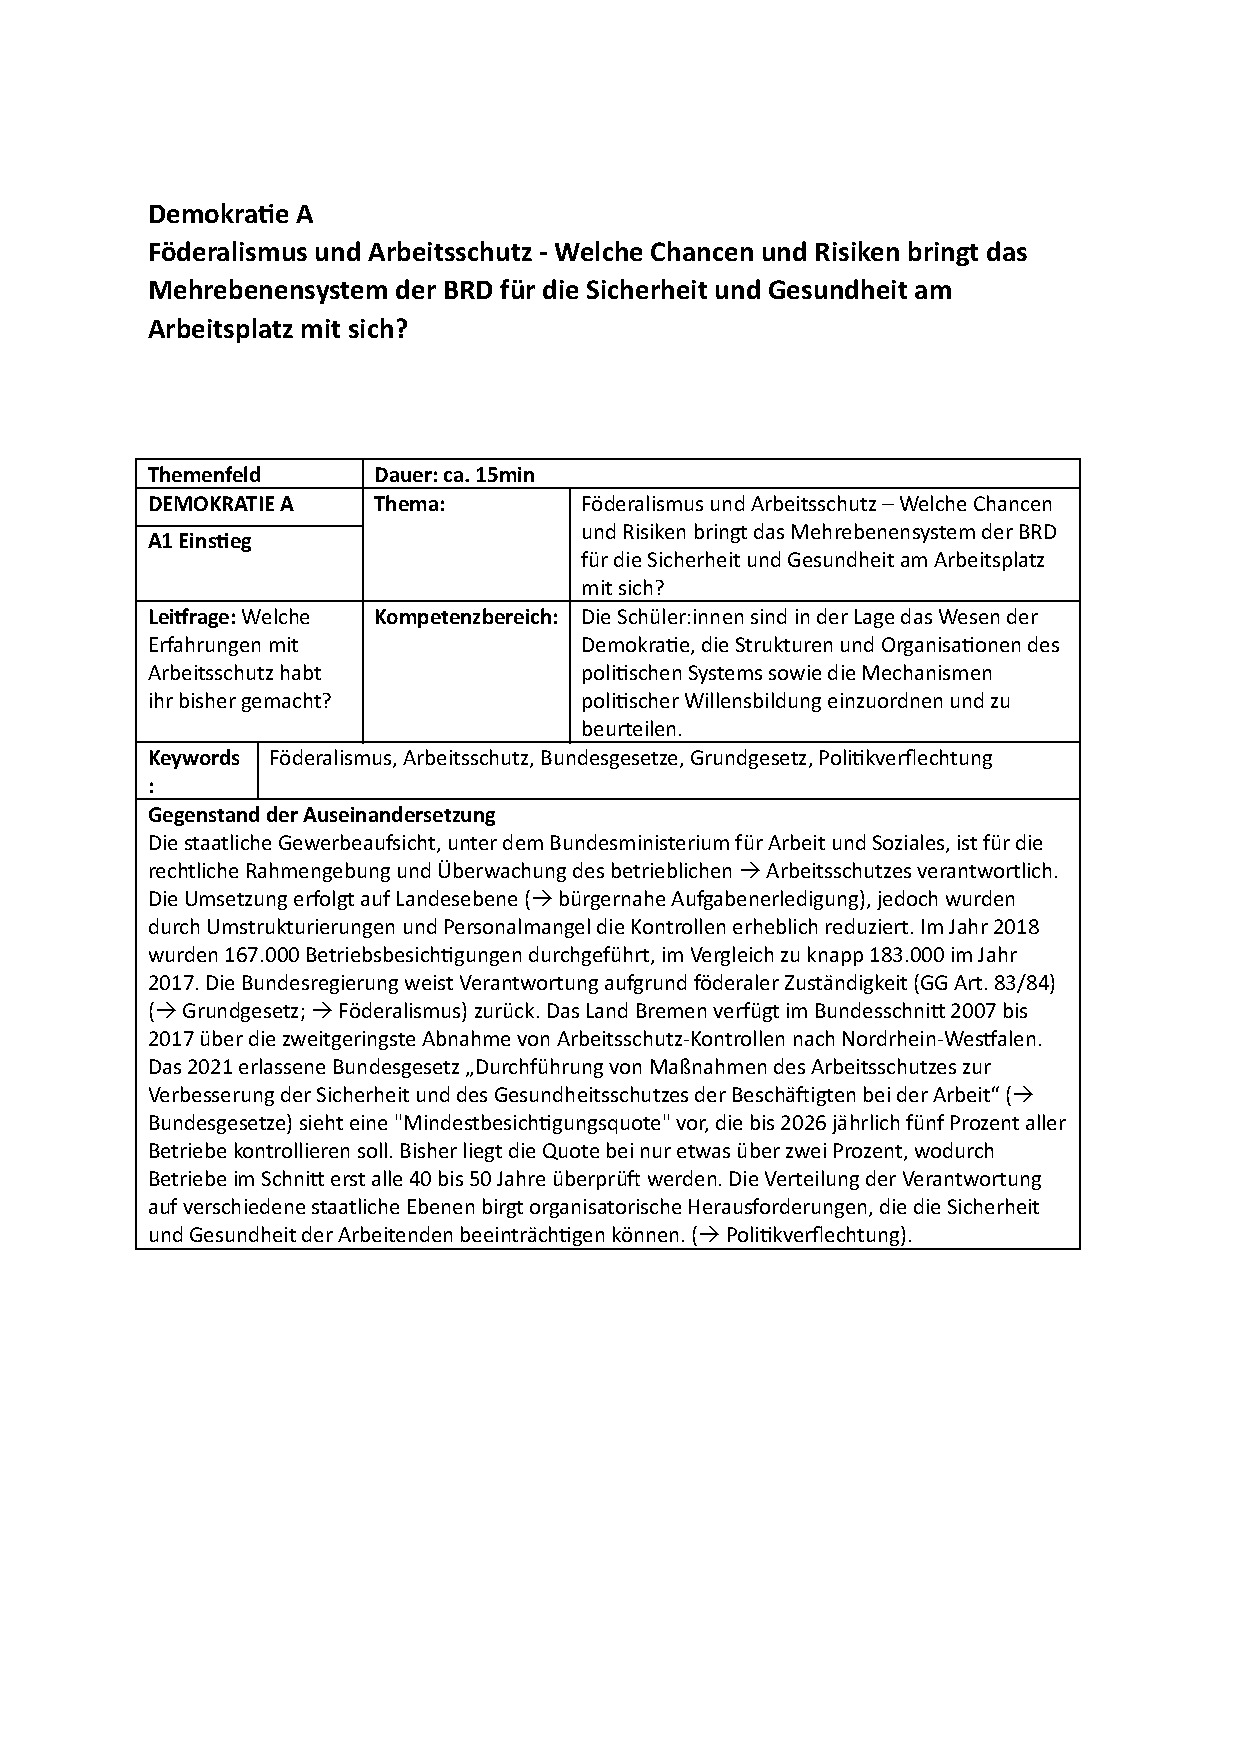
\includepdf[
    nup=2x1, 
    addtotoc={
    1, subsection, 2, Demokratie A1, DEMOKRATIE-A1, 
    3, subsection, 3, Demokratie A2, DEMOKRATIE-A2, 
    6, subsection, 2, Demokratie A3, DEMOKRATIE-A3, 
    9, subsection, 2, Demokratie B1, DEMOKRATIE-B1, 
    11, subsection, 2, Demokratie B2, DEMOKRATIE-B2, 
    13, subsection, 2, Demokratie B3, DEMOKRATIE-B3
    }
]
{DEMOKRATIE.pdf}

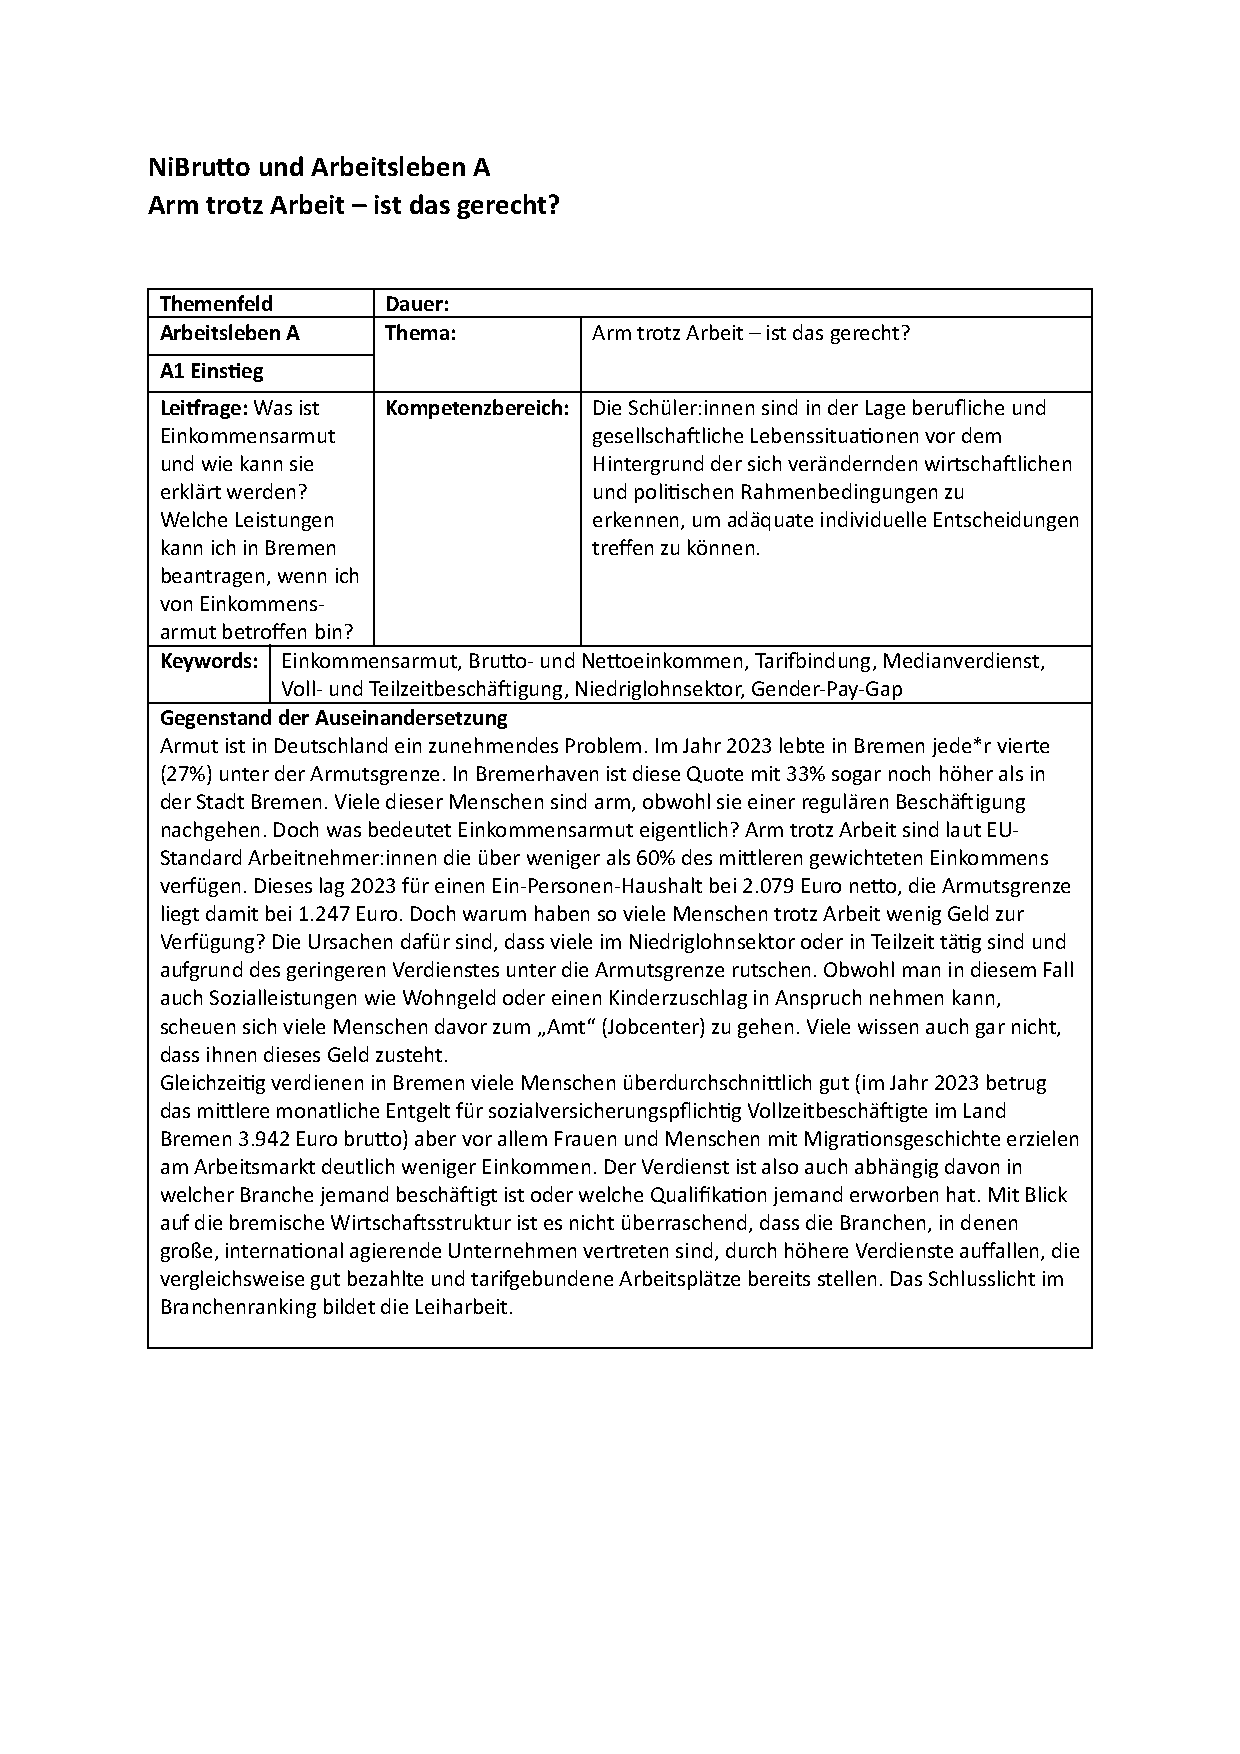
\includepdf[
    nup=2x1, 
    addtotoc={
    1, subsection, 2, Arbeitsleben A1, ARBEITSLEBEN-A1, 
    3, subsection, 2, Arbeitsleben A2, ARBEITSLEBEN-A2, 
    5, subsection, 2, Arbeitsleben B1, ARBEITSLEBEN-B1, 
    7, subsection, 2, Arbeitsleben B2, ARBEITSLEBEN-B2, 
    9, subsection, 2, Arbeitsleben B3, ARBEITSLEBEN-B3, 
    11, subsection, 2, Arbeitsleben C1, ARBEITSLEBEN-C1, 
    12, subsection, 2, Arbeitsleben C2, ARBEITSLEBEN-C2
    }
]
{ARBEITSLEBEN.pdf}

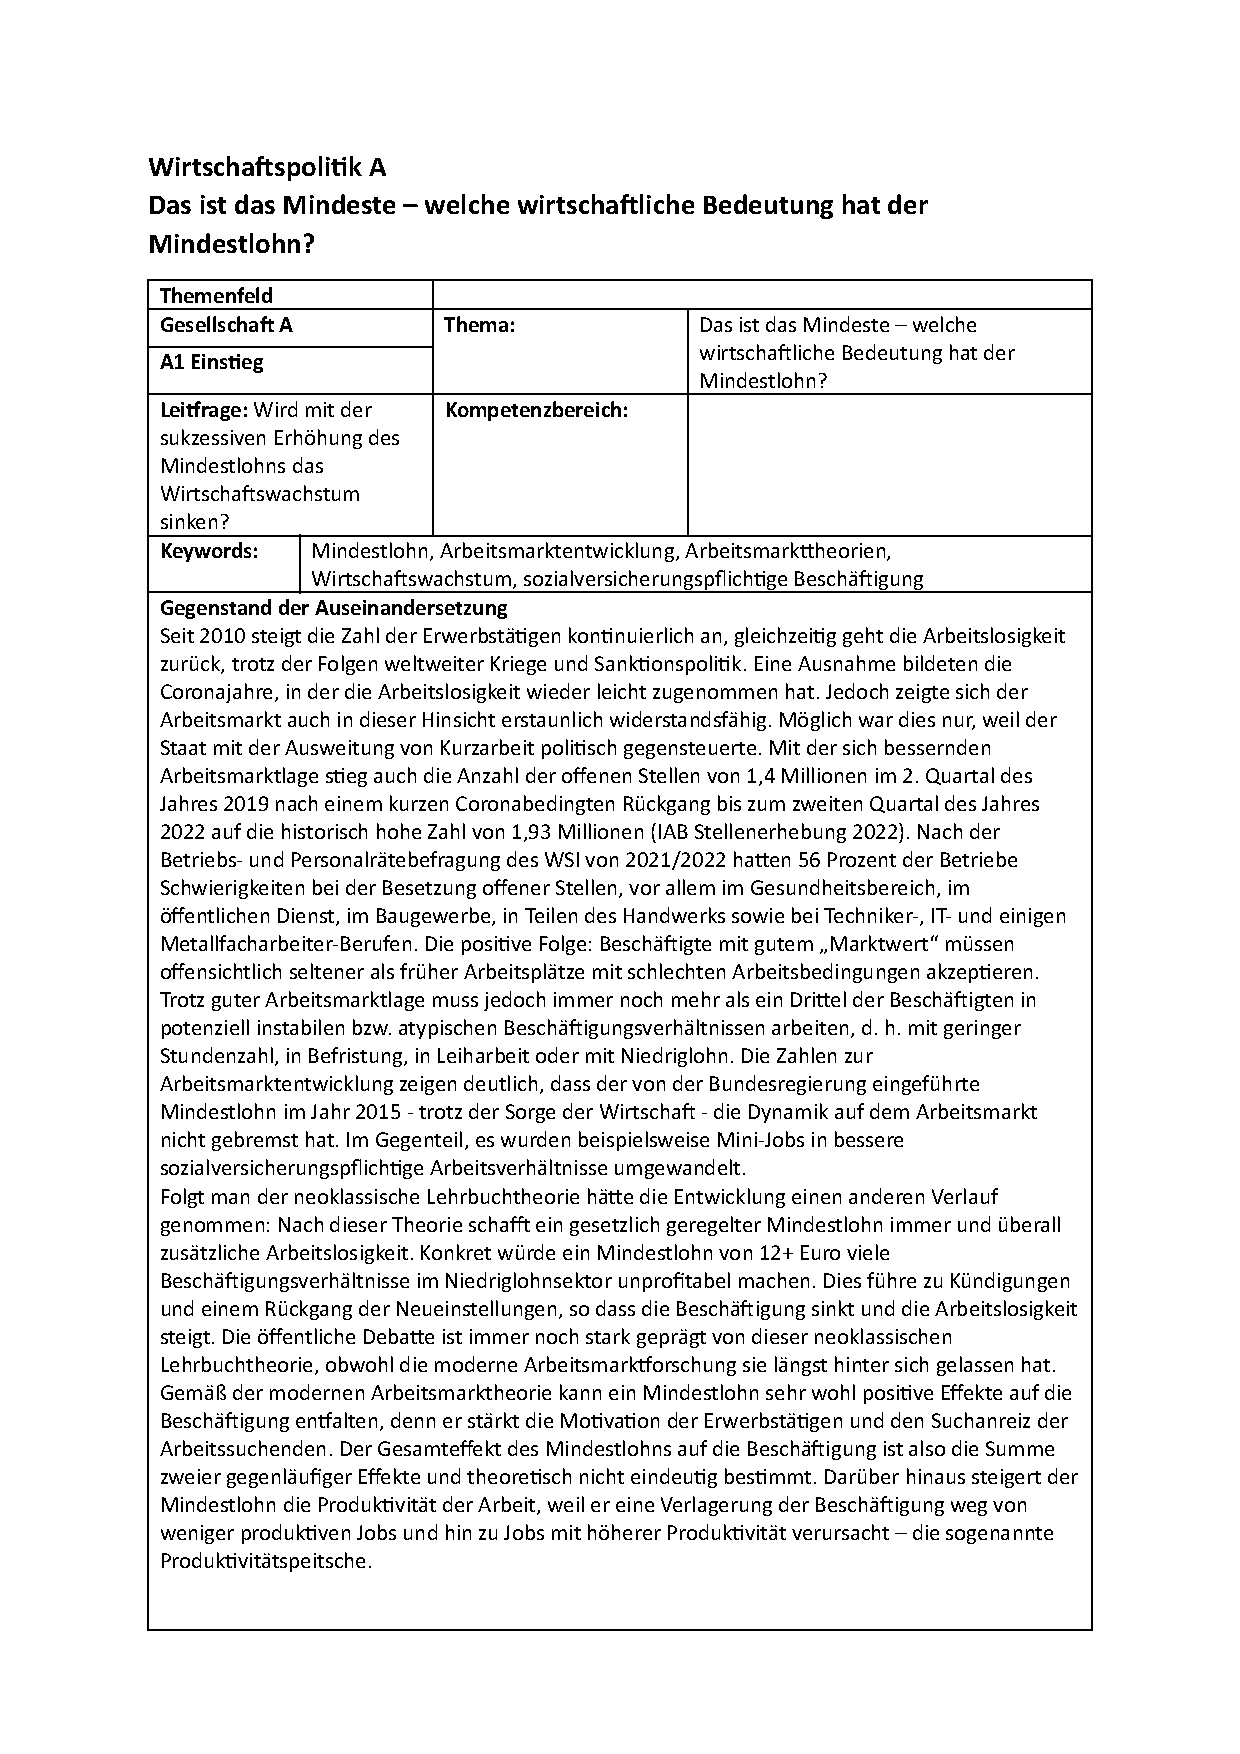
\includepdf[
    nup=2x1, 
    addtotoc={
    1, subsection, 2, Wirtschaftspolitik A1, WIRTSCHAFTSPOLITIK-A1, 
    3, subsection, 2, Wirtschaftspolitik A2, WIRTSCHAFTSPOLITIK-A2, 
    5, subsection, 2, Wirtschaftspolitik A3, WIRTSCHAFTSPOLITIK-A3, 
    7, subsection, 2, Wirtschaftspolitik B1, WIRTSCHAFTSPOLITIK-B1, 
    9, subsection, 2, Wirtschaftspolitik B2, WIRTSCHAFTSPOLITIK-B2, 
    11, subsection, 2, Wirtschaftspolitik C1, WIRTSCHAFTSPOLITIK-C1, 
    13, subsection, 2, Wirtschaftspolitik C2, WIRTSCHAFTSPOLITIK-C2
    }
]
{WIRTSCHAFTSPOLITIK.pdf}

%%%%%%%%%%%%%%%%%%%%%%%%% from page 7-8 of: https://texdoc.org/serve/pdfpages.pdf/0
% Experimental options: (Syntax may change in future versions!)
% addtotoc Adds an entry to the table of contents. This option requires five arguments, separated by commas:
% addtotoc={⟨page number⟩,⟨section⟩,⟨level⟩,⟨heading⟩,⟨label⟩}
% ⟨page number⟩: Page number of the inserted page.
% ⟨section⟩: LATEX sectioning name– e.g., section, subsection, …
% ⟨level⟩: Number, denoting depth of section– e.g., 1 for section level, 2 for
% subsection level, …
% ⟨heading⟩: Title inserted in the table of contents.
% ⟨label⟩: Name of the label. This label can be referred to with \ref and \pageref.

% Note: The order of the five arguments must not be mixed. Otherwise you will get very strange error messages.
% The addtotoc option accepts multiple sets of the above mentioned five arguments, all separated by commas. The sets must be sorted such that the ⟨page number⟩s are in ascending order. (Strictly speaking they must have the same order as the page numbers specified by the pages option.)
% The proper recursive definition of the addtotoc option is:
% addtotoc={⟨toc-list⟩}
% ⟨toc-list⟩ → ⟨page number⟩,⟨section⟩,⟨level⟩,⟨heading⟩,⟨label⟩[,⟨toc-list⟩]

\clearpage
\newpage


\section{Dokumentation der Nutzung von KI-basierten Anwendungen und Werkzeugen}
Die folgende Tabelle wurde in Anlehnung an die Vorlage der Universität Bremen erstellt:
\\

\footnotesize{
    \url{https://www.uni-bremen.de/zpa/formulare} führt zu: 
    \\

    \url{https://view.officeapps.live.com/op/view.aspx?src=https%3A%2F%2Fwww.uni-bremen.de%2Ffileadmin%2Fuser_upload%2Fsites%2Fzpa%2Fpdf%2Fallgemein%2FDokumentation_Nutzung_KI_-_AI_Use_Documentation.docx&wdOrigin=BROWSELINK} 
    \\
    
    beide 29.06.2025
    }

% Adaptive column width and multipage support using longtable and tabularx

\clearpage

\newgeometry{left=10mm, right=10mm, top=10mm, bottom=20mm}

\begin{landscape}
\begin{longtblr}[
    caption = {Dokumentation der Nutzung von KI-basierten Anwendungen und Werkzeugen -- Documentation of the Use of AI-based Applications and Tools},
    label = {KIHilfsmittel}]
    {colspec={| c |[1.2pt] X |[dashed] X |[dashed] X |[dashed] X |[dashed] X |}}
\hline
                                & 
    KI-basiertes Hilfsmittel 
        
    AI-based Tool               & 
    Einsatzform 

    Purpose                     & 
    Betroffene Teile der Arbeit 
        
    Aspect of the Work Affected & 
    Beschreibung der Eingabe (Prompt) 
  
    Prompt (Entry)              & 
    Bemerkung 
    
    Comment                     \\ 
    \hline[1.2pt]

    
    1                                                                                                                                           & 
    GitHub Copilot (Chat) in Visual Studio Code

    Inline Chat \& Chat on Secondary Sidebar

    mostly with GPT-4.1 as \gls{llm}                                                                                                            & 
    Fragen zu \LaTeX{} Code, keine inhaltlichen Fragen                                                                                          &
    alle, insbesondere \gls{zb} der Code zur Form dieser Tabelle oder Fragen zum Darstellen von eingebunden PDF-Seiten im Inhaltsverzeichnis    & 
    \gls{zb} \enquote{ia there \textbackslash{}vfill in latex?},  
    
    \enquote{what does \textbackslash{}arraybackslash in tabularx do?}, 
    
    \enquote{what can the parameter in lines 14 or 27 change?} oder
    
    \enquote{how do I make several entries to the toc like I treid in lines 26 to 62?}
    
    \enquote{welches paket in latex für mehrseitige tabellen?} \gls{etc}                                                                        & 
    Es werden nicht alle Prompts aufgeführt. Es wurde ausschließlich für den Code Hintergrund benutzt und nie für den Inhalt. 
    
    Das Meiste wurde dann ohnehin doch wieder über Suchmaschinen und dann Foren und Anleitungen lesen erledigt. Häufig eben erst im Anschluss an das initiale Ausprobieren von \gls{ki} \\ 
    \hline
    %%%%%%%


    2                                                                                                                               &
    Visual Studio Code Autovervollständigung                                                                                        &
    Codevervollständigung und Autovervollständigung von einzelnen Worten, ähnlich dem Tippen auf Smartphones                        &
    alle                                                                                                                            &
    keine Prompts. 
    
    Bei der Eingabe \enquote{Effiz} wird dann \gls{zb} \enquote{Effizienz} vorgeschlagen und nach Druck auf Enter ausgeschrieben    &
    Die Grenze von maschinellem Lernen und Skripts oder überhaupt Software Hilfsmitteln ist fließend. Auch wenn schon länger existierende Autovervollständigungen für einzelne Worte keinen \gls{ki}-Boom und derartige gesellschaftliche Diskurse ausgelöst hat, wie es die \gls{llm} derzeit hervorrufen.                                             \\ 
    \hline

% \pagebreak

    3                                               &
    ChatGPT.com                                     &
    Erstellen einer Graphik                         &
    \gls{abb} \ref{Absetzungsbetrag} auf \gls{S} \pageref{Absetzungsbetrag}                                      &
    \enquote{Bitte plotte  die vier Funktionen unten in einer Abbildung. Beschrifte die x-Achse in hunderter Schritten. Mach keine Überschrift. Nenne die x-Achse anzurechnendes Einkommen in €. Nenne die y-Achse Absetzungsbetrag in € \\

    f (x) = x Df = {0 < x < 100} (1) \\

    f (x) = 0, 2x + 80 Df = {100 < x < 520} (2) \\

    f (x) = 0, 3x + 28 Df = {520 < x < 1000} (3) \\

    f (x) = 0, 1x + 228 Df = {1000 < x < 1200} (4)}
                                                    &
    Danach wurde mit weiteren Prompts das Aussehen der Grafik noch weiter verfeinert. Weil ich mir kein ChatGPT Plus oder Pro leisten kann, wurden mir keine Grafiken mehr ausgegeben. Also wurde Python installiert, der generierte Code kopiert und in Visual Studio Code eingefügt, um eine Grafik mit gleichmäßiger Skalierung auf dem eigenen Rechner zu erstellen.\\
    \hline

\end{longtblr}
\end{landscape}

\restoregeometry

% \footnote{\url{https://www.uni-bremen.de/zpa/formulare} führt zu \url{https://view.officeapps.live.com/op/view.aspx?src=https%3A%2F%2Fwww.uni-bremen.de%2Ffileadmin%2Fuser_upload%2Fsites%2Fzpa%2Fpdf%2Fallgemein%2FDokumentation_Nutzung_KI_-_AI_Use_Documentation.docx&wdOrigin=BROWSELINK} beide 29.06.2025}
\end{document}